\documentclass{MSthesis} 
% subclass of the document class report.

\begin{document}

% Formatting titles and spaces 

% Originally its
% Chaper 1:
% Name of chapter one
\titleformat{\chapter}[hang] 
{\normalfont\huge\bfseries}{\thechapter}{1em}{}  

% left margin, vertical space,  space to section, 
\titlespacing*{\chapter}{0cm}{0cm}{0cm}
\titlespacing*{\section}{0cm}{0cm}{0cm}
\titlespacing*{\subsection}{0cm}{0cm}{0cm}
\titlespacing*{\subsubsection}{0cm}{0cm}{0cm}
%%%%%%%%%%%%%%%%%%%%%%%%%%%%%%%%%%%%%%%%%%%%%%%%

% USING THE TWOSIDED OPTION left = inner , and right = outer
\myfrontpage
\mycopyright

%\newpage\null\thispagestyle{empty}\newpage

% Abstract should have first page nr,
\pagenumbering{roman}
\chapter*{Abstract}
\addcontentsline{toc}{chapter}{Abstract}

\subsection*{Introduce topic and why its important}
Helicopters being hit by lightning is a real threat faced by many offshore personnel in the winter months. This study assesses the available theoretical explanations to this phenomenon and looks at the meteorological situation when such an incident has occurred.

\subsection*{Introduce a challenge or unresolved issue that you will try and solve.} 
The current forecasting algorithm does not always show high risk when helicopters are being hit by lightning or static discharges. It has been reported to show high risk when no meteorological phenomena related to risk are present.

\subsection*{What have you done to try and solving this.}
This thesis investigate the parameters being used in forecasting \acrfull{htl}, and tries to verify the algorithm with use of cases of lightning strikes to aircraft. 


\subsection*{The implications in the context of 1+2.}
The error in the forecast has given a overforecasting along coastal areas, where the vertical velocity and temperature part of the forecast often was present. This caused a possible overestimation of risk.

\chapter*{Acknowledgements}
\addcontentsline{toc}{chapter}{Acknowledgement}
It is with great honor I now present the product of two amazing years as a Master student. This thesis could not have been completed without considerable help from various people around me. Special thanks goes to my supervisors Trude Storelvmo and Morten Køltzow. For their supervision and helpful guidance, and not least their constructive criticism of my writing style. I would be remiss not to thank Johanne Mehren for tipping me off to the opportunity of this project, and of course for her friendship and jokes (Even or maybe especially those on my behalf).

I am of course indebted to Martin Boie Christiansen and Glenn Christiansen for their help and interest in this project. Their insights into the world of helicopters have been essential. I still am awaiting their offer to let me fly in one of their helicopters. 

The thesis was also written in a time of great global turmoil, as the world was hit by the COVID-19 pandemic. This in turn leads me to thank the Rian Julsrud family for their hospitality in letting me isolate from the rest of the world in their cellar. It is not an understatement that I have learned and continue to learn immensely by our talks at the coffee- and dinner tables.

The list of people who I owe thanks to contains a myriad of names. I would love to list them all but, the paper usage would not be defensible. Instead I would thank a special few who is not aforementioned: My mother and father, my American proofreader and friend Jonah Shaw, my brothers Tobias and Alphonse, and the Ingeborg(s) \\

\begin{center}
\textbf{Johannes Tobiassen Langvatn}
\end{center}
\begin{center}
\textbf{July 2020}
\end{center}
\includecomment{, and last but never least, my friend Leila who passed during the work of this thesis.}

\includecomment{
-Acknowledge Martin Boie Christiansen
-Avinor
-Morten and Trude
-The jussruds
}

\tableofcontents

% Clear double page --> New chapers or listings begin on odd numbered pages.
\cleardoublepage

\listoffigures
\addcontentsline{toc}{chapter}{\listfigurename}
\cleardoublepage

% List of tables 
\listoftables
\addcontentsline{toc}{chapter}{\listtablename} % add list of tables to contents line
\cleardoublepage

% List of acronyms
\printglossary[type=\acronymtype]
\addcontentsline{toc}{chapter}{Acronyms}

\newacronym{ic}{IC}{Intracloud discharge}
\newacronym{cg}{CG}{Cloud-to-ground discharge}
\newacronym{htl}{HTL}{Helicopter triggered lightning}
\newacronym{fwtl}{FWTL}{Fixed wing triggered lightning}
\newacronym{hti}{HTI}{Helicopter trigger index}
\newacronym{meps}{MEPS}{MetCoOp ensemble prediction system}
\newacronym{era5}{ERA5}{ECMWF atmospheric reanalysis}
\newacronym{nwp}{NWP}{Numerical weather prediction}
\newacronym{ecmwf}{ECMWF}{European Centre for Medium-Range Weather Forecasts}
\newacronym{oat}{OAT}{Outside air temperature}
\newacronym{metar}{METAR}{Meteorological aerodrome report}
\cleardoublepage

\pagenumbering{arabic} % page numbering to arabic
\chapter{Introduction and Motivation}\label{ch:introduction}

Helicopters are a vital part of the transport of personnel to offshore installations along the Norwegian coast. Offshore personnel report fear of being involved in helicopter incidents. They also experience unease from flying in turbulent and bad weather (\cite{wasilewska2019}). These weather types may be causal to incidents, as suggested in earlier work (e.g. \cite{lande1999}; \cite{wilkinson2013}; \cite{smart1997}). It is therefore imperative to exhaust the investigation into the causes of and possible ways to prevent helicopter related incidents. 
Helicopters flying offshore in the higher latitudes of the northern hemisphere are sometimes hit by lightning. This can in various ways be the cause of incidents. These incidents include events when rotors have been destroyed, as in the case of Flight 56 in 1995 (\cite{smart1997}). Sometimes a breakdown of the structural integrity of a rotor by lightning is not discovered right away, but can still be serious. For example, a lightning strike in 1999 is believed to have caused a fatal crash in 2002 (\cite{smart2005}). Incidents of less fatal variety include disruption to electrical equipment (Table 10.2. \cite{rakovBok}). Flying helicopters are in practice only hit by lightning in wintertime, (See Figure \ref{fig:landewilk}) and this phenomenon is referred to as \acrfull{htl} (e.g. \cite{lande1999}; \cite{wilkinson2013}). The triggering refers to the helicopters being hit by lightning in areas where there is little to no lightning activity before the lightning strike. When there is lightning activity present, a helicopter pilot avoids the area (further discussed in section \ref{sec:data}).


\begin{figure}
    \centering
    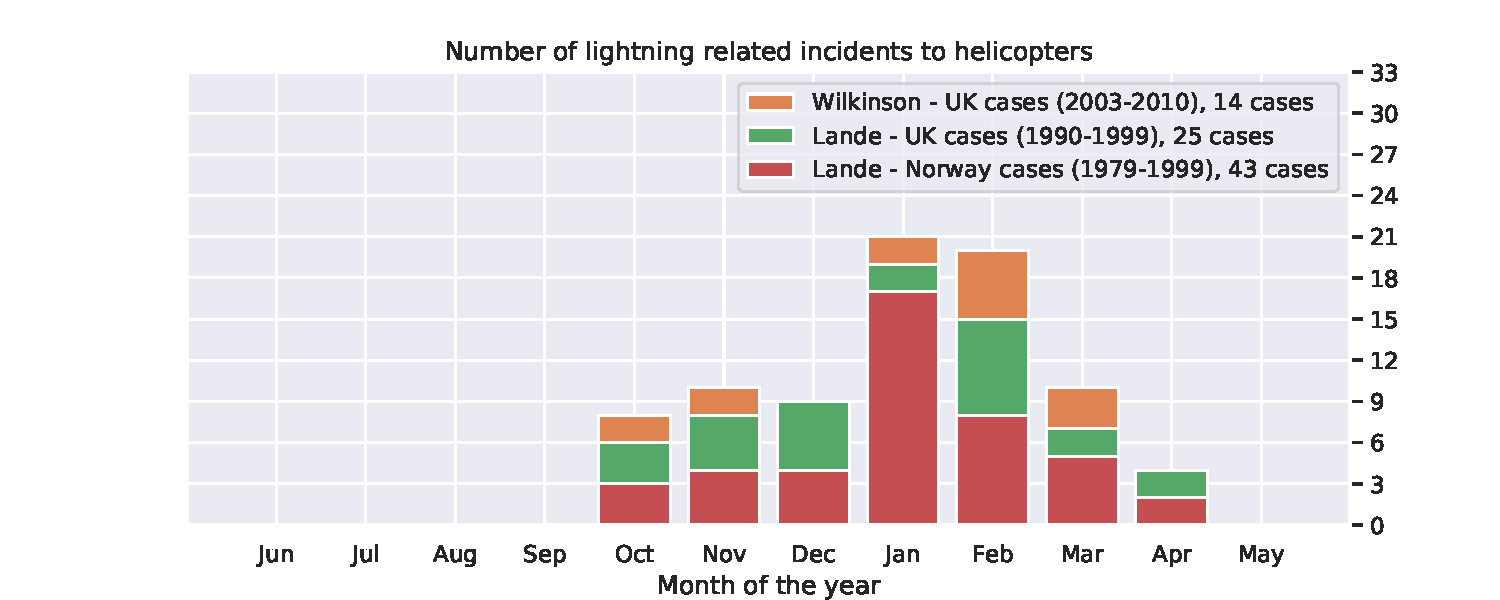
\includegraphics[width=\textwidth]{Figures/yearlydistribution_withoutmine.pdf}
    \caption{Seasonal variation of helicopter cases, showing no cases in May to September. Data is produced from \cite{lande1999} and \cite{wilkinson2013}. Legend notes time-periods and amount of cases in each study.}
    \label{fig:landewilk}
\end{figure}

The study of \acrshort{htl} had its peak around the turn of the century, due to two helicopter incidents related to lightning (1995 and 2002). The 1995 incident was a non-fatal incident. A lightning strike destroyed the main rotor of the helicopter, forcing the pilot to perform a landing in the ocean (\cite{smart1997}). The 2002 incident resulted in eleven fatalities and is believed to have been caused by internal damage to the helicopter's main rotor back in 1997. The initial inspection of the rotor did not uncover any damage, causing the helicopter to be cleared for flight. This initial structural damage later resulted in failure of the main rotor, leading to the crash in 2002 (\cite{smart2005}). These events resulted in practical guidelines to helicopter pilots based on data from earlier incidents (\cite{lande1999}, \cite{hardwick1999}). Furthermore, the UK Met Office added numerical simulation and forecasting to these guidelines, with the introduction of \acrfull{hti}. This provided a more robust warning for helicopter pilots (\cite{wilkinson2013}). Since then, general \acrfull{nwp} forecasts have improved and continue to improve due to better  physical understanding, more and higher quality observations, and increase in available computational power. This thesis aims to improve upon the understanding of the \acrshort{htl} phenomenon by using state-of-the-art model products.

The author makes use of a novel dataset from Avinor containing reported incidents of both  \acrshort{htl} and a similar phenomenon: \acrfull{fwtl}. \acrshort{fwtl} is triggered lightning involving planes and rockets, where the wings are fixed. \acrshort{fwtl}, unlike \acrshort{htl}, is of less danger to both personnel and materials. Fixed wing aircraft are generally hit in the main body. Fuel and vital electronics are also better protected in fixed wing aircraft (\cite{petrov2012}). Helicopters are mainly hit through the rotor into the main body (\cite{lande1999}). Despite this difference in actual risk, both incidents are associated with non-negligible risk, and require thorough inspection of the aircraft after the fact.

To investigate atmospheric conditions during \acrshort{htl} and \acrshort{fwtl} incidents, the \acrfull{era5} dataset is utilized. Also used for this purpose is the operational \acrfull{meps}. \acrshort{meps} became available in November 2016, and hence can only provide atmospheric conditions for cases that have occurred since then. \acrshort{meps} provides higher spatial resolution compared to \acrshort{era5}. Further, the \acrshort{meps} ensemble members are evaluated in order to assess if this can provide improved forecast ability for \acrshort{htl}.

These are the research questions this thesis attempts to answer:
\begin{itemize}	
    \item What atmospheric conditions are present for an \acrshort{fwtl}-event and can \acrshort{fwtl} be used as a proxy for \acrshort{htl}? 
    \item Is \acrshort{htl} forecasted well?
    \item In what ways can the \acrshort{htl} forecast be improved?
\end{itemize}

The goal is to improve and strengthen the confidence in the current operational \acrshort{htl} forecast. Also under investigation is an error found in the algorithm used to produce the operational forecast where the accumulated precipitation, and not the intended hourly precipitation, was used in the operational forecast. This lead to a potential over-estimation of risk related to offshore flights.

\section{Layout of the thesis}

The theory builds on the historical context, but also introduce the physical mechanisms of lightning-producing storms. In section ... this is used to investigate the physical mechanisms believed to be present in a winter-lightning situation. This again is related to \acrfull{htl} in section ... and how a short discussion about the challenges related to forecasting this phenomenon is had.

The method chapters discussed the data and methods used in this thesis. The first section (sec....) is dedicated to detailing the models producing the data used. Section ... then details the dataset received from Avinor. Lastly section ... describes the methods used in this thesis, ranging from the already implemented algorithm, to statistical sizes used in this thesis.

The results chapter starts off with investigation into the temporal and spatial spread of the cases of lightning incidents to aircraft. This is then followed by a section on the atmospheric conditions during these cases. These atmospheric conditions are then investigated in the operational model. Lastly a preliminary investigation into usage of EPS is performed.

The conclusion relates the discussion to earlier works.




\cleardoublepage

\setcounter{chapter}{1} 

\chapter{Lightning}

\section{Natural Lightning}
The study and observations of lightning has a very long history, but only in the last century have we acquired the means to thoroughly investigate the electrical and meteorological mechanisms resulting in a thunderstorm.

There are varying theories in  the still open field of thunderstorms. The electrification mechanisms and the general electrical structure of the convective thunderstorms. This is further complicated by the fact that there seems to be different mechanisms at work for different scales of convective systems. Alas, every thunderstorm is a cloud, so it is necessary to explain cloud creation mechanisms.

The \textit{typical} lightning storm is created in summertime, this is caused by incoming solar radiation heating up the ground, and creating an unstable atmosphere.

The instability can be understood by recognizing that warm air is lighter than cold air, and therefore will rise. When air rises, less pressure is exerted on it, since the atmosphere is densest at the surface. This lower pressure causes work to be done by the rising air, to expand to a new equilibrium. The work done by the air in form of expansion, leads to a cooling of the air mass.

This instability is cause to a vertical movement. This vertical movement carries with it humid air. When the air mass is cooled by the expansion, the ability to hold water vapor is decreased (CC), and this may lead to condensation of vapor into liquid water in form of cloud droplets. Condensation of water vapor heats the surrounding air, which gives more vertical movement.

There are two mechanisms of electrification believed to be dominant (e.g \cite{saunders2007}, \cite{soula2012}). Collision of different sized ice-particles and collision of smaller ionized particles with a hydrometeor. (Beskriv disse mer)

Lightning discharges in a thunderstorm can generally be divided into two categories (e.g. \cite{lynn2011}): \acrfull{ic} and \acrfull{cg}, see figure \ref{fig:lyntyper} for description and comparison. A \acrshort{cg} is seen developing downwards before making contact with the ground. The stream of electrons developing downwards is what is referred to as a leader (\cite{rakovBok}). On the other hand, \acrshort{ic} does not have this leader, since the distance between charged parts of the cloud are closer to each other than to earth.

\begin{figure}
    \centering
    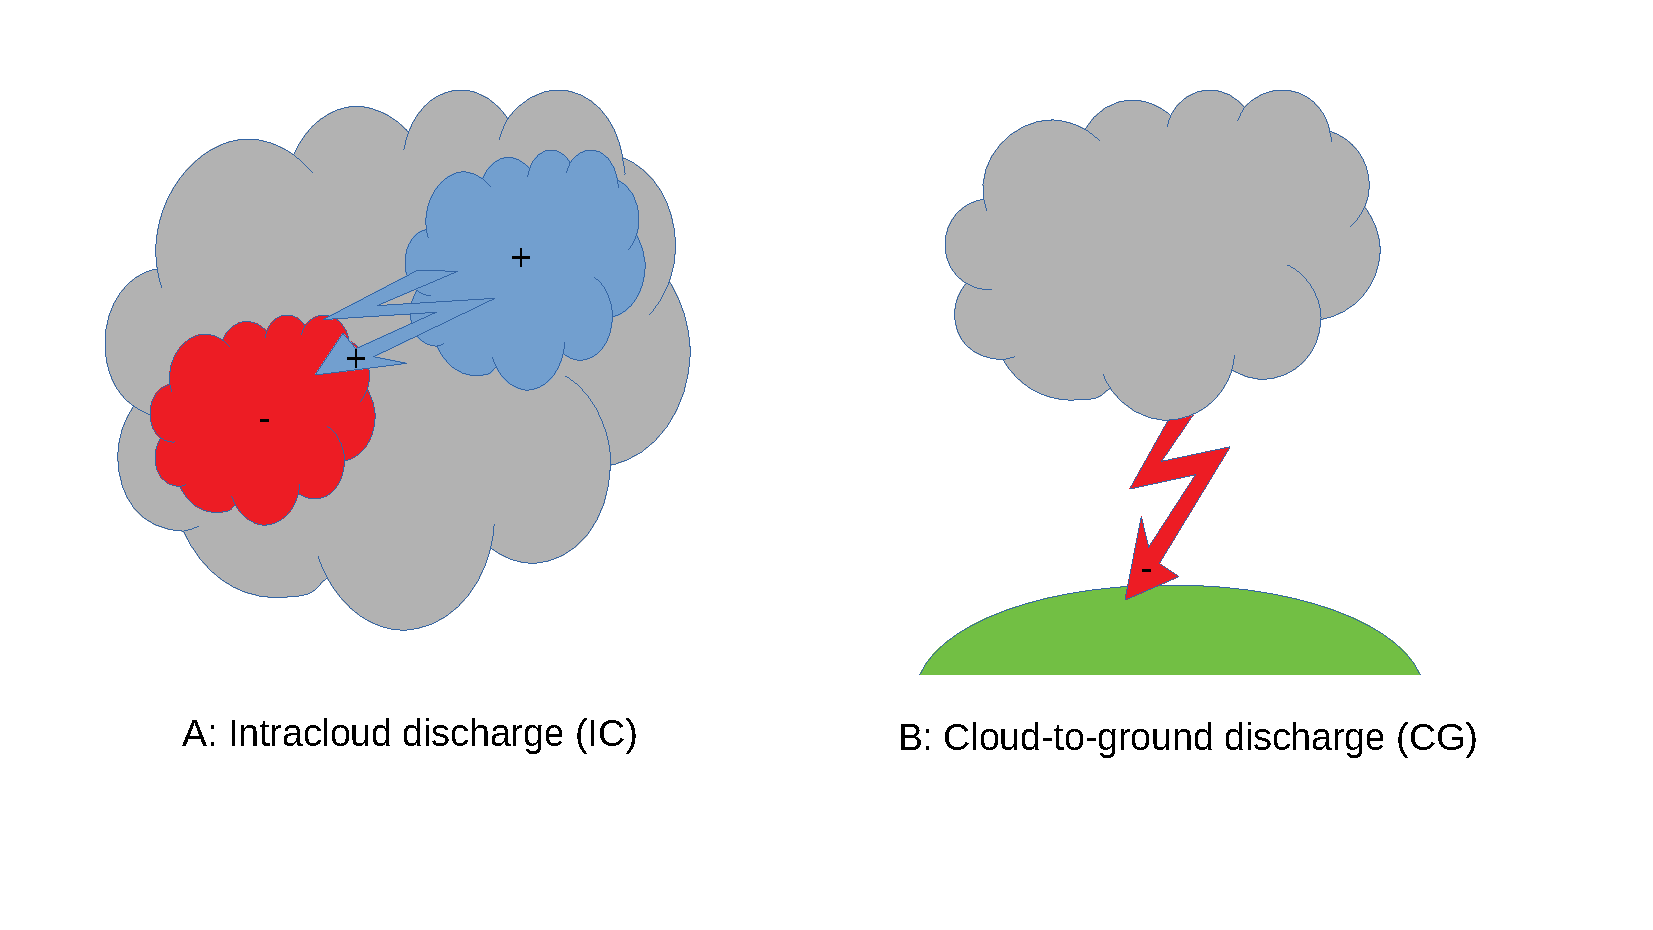
\includegraphics[width=\textwidth]{Figures/lyntyper.pdf}
    \caption{The two main categories of lightning. A shows an \acrfull{ic}, this could be between different storm cells or between different charge areas of the same storm cell. B shows a \acrfull{cg}, the polarity is defined by the charge change of earth. Negative cloud-to-ground (-CG) is defined by increase of negative charge at ground, and so positive cloud-to-ground (+CG) is defined by decrease of negative charge (increase in positive) at ground}
    \label{fig:lyntyper}
\end{figure}


\subsection{Winter lightning}
A phenomenon has been described in the Japanese meteorological field, where cold air from Siberia moves over the warm Tsushima current on the west coast of Japan. This leads to a strong temperature gradient between the cold air and the warm ocean, which causes convection. The  humidity supplied by the seawater leads to formation of hydrometeors. The resulting convection has been shown to produce lightning strikes and thunderstorms during winter (e.g. \cite{goto},\cite{michimoto2007}).

A similar phenomenon is observed of the west coast of Norway (e.g \cite{koeltzow2018}, \cite{montanya2016}). Cold air is brought from the arctic to the west coast of Norway where the ocean is warmed by the North Atlantic Current.The resulting temperature gradient may give rise to a convection and subsequent electrification.
 %This updraft and the creation of hydrometeors leads to an electrification that results in the aforementioned thunderstorms. 
 
\section{Helicopter Triggered Lightning}
An \acrshort{htl} is believed to be a phenomenon caused by the helicopter entering or coming close to an electrically charged part of a convective system. This can be attributed to the helicopter having a charge build-up during flight and then meeting a charge of opposite polarity. Alternatively the helicopter could induce a \acrshort{cg} by acting as part of the leader, see figure \ref{fig:triggertyper}. These different mechanisms are then analogous to \acrshort{ic} and \acrshort{cg} respectively. 

A positively charged discharge is believed to cause more damage to helicopters. The discharges to helicopters are also more often positive  (\cite{hardwick}).
%Helicopter triggered lightning is unique in that it does not occur during summertime, but only during the winter months (\cite{lande},\cite{wilkinson}).

\begin{figure}
    \centering
    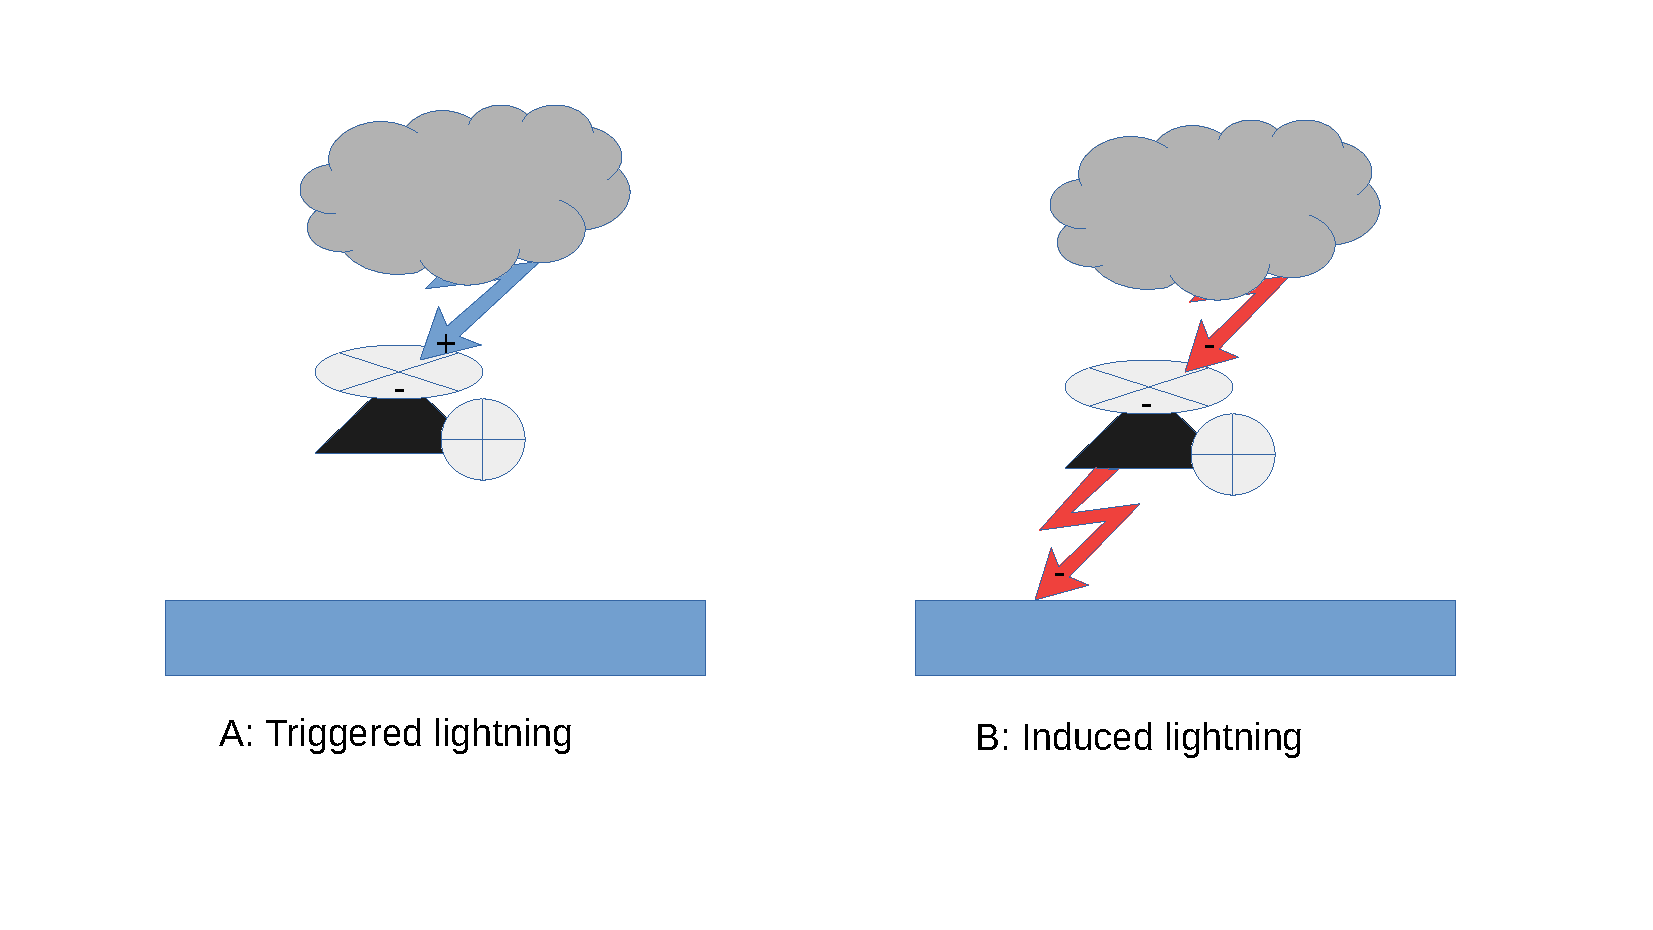
\includegraphics[width=\textwidth]{Figures/triggertyper.pdf}
    \caption{Illustration of different models for aircraft triggering. A shows the normal trigger situation, where the electrical discharge is grounded into the oppositely charged aircraft. B shows the situation where the aircraft is only acting as a pathway to the ground (Here ocean or land)}
    \label{fig:triggertyper}
\end{figure}

\subsection{Fixed Wing Triggered Lightning}

\acrfull{fwtl}, unlike \acrshort{htl}, is of less danger to both personnel and materials. Fixed-wing aircraft are generally hit in the main body. Fuel and vital electronics are also more protected in fixed-wing aircraft (\cite{Petrov12}). Helicopters are mainly hit through the rotor into the main body (\cite{lande}). 


\subsection{Forecasting HTL}
(\cite{lande}) looked at the common atmospheric conditions present for a \acrshort{htl}:
\begin{itemize}
 \item \acrfull{oat} at flight level near freezing point 
 \item frozen precipitation, as snow,ice and graupel.
 \item inside of or directly below clouds.
 \item within 5 nautical miles of a Cumulonimbus cloud.
\end{itemize}
This corresponds to convective activity, and especially zones of high electrification (Electrification is highest in the $0 - -10^{\circ}C$ temperature range. So what we want to find is local convective areas over oceans.




\cleardoublepage

\setcounter{chapter}{2}
\chapter{Methods}

Example table from \href{https://www.tablesgenerator.com/#}{https://www.tablesgenerator.com/}.
\begin{table}[]
    \centering
    \begin{tabular}{ccc}
    \hline
    Animal     & Description & Price (\$) \\ \hline
    Gnat       & per gram    & 13.65      \\
               & each        & 0.01       \\
    Gnu        & stuffed     & 92.50      \\
    Emu        & stuffed     & 33.33      \\
    Armadillo  & frozen      & 8.99       \\ \hline
    \end{tabular}
    \caption{Grocery store prices. }
    \label{tab:gros}
\end{table}

Referencing table \ref{tab:gros}.
\cleardoublepage

\chapter{Results and discussion}

\section{Analysis of Avinor triggered lightning data set}\label{sec:avinor}

\begin{figure}
    \centering
    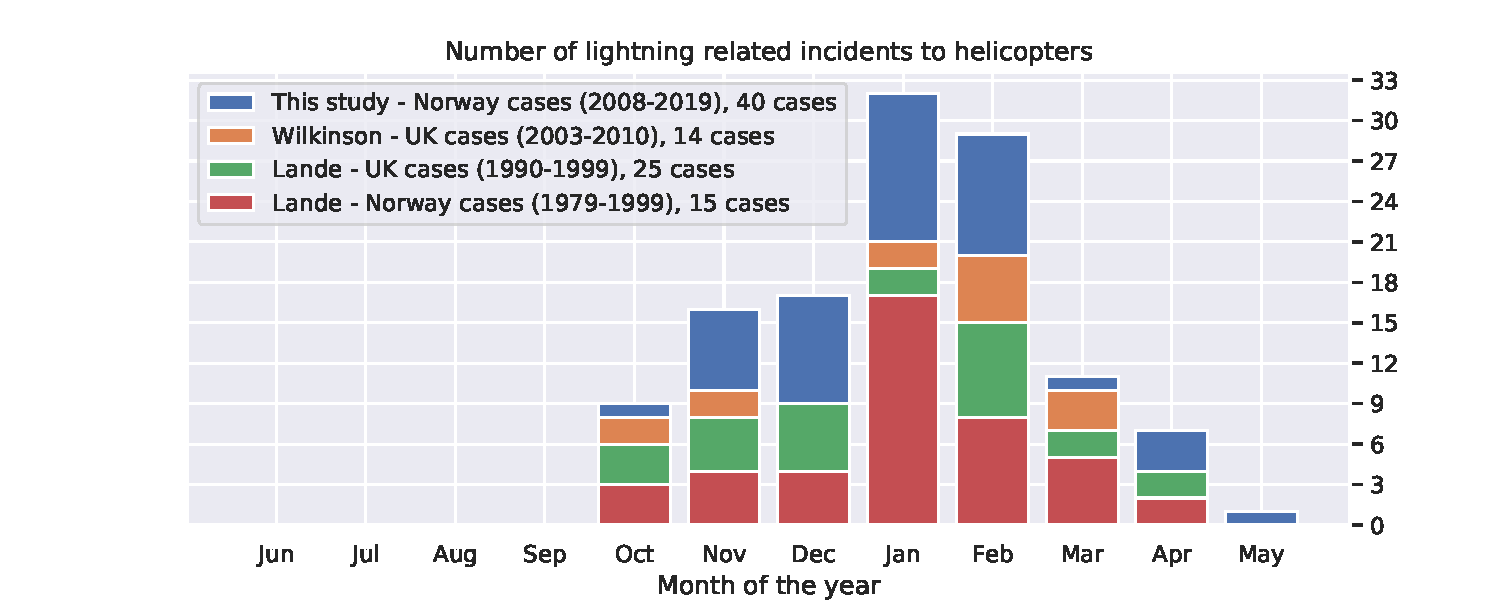
\includegraphics[width=\textwidth]{Figures/yearlydistribution.pdf}
    \caption{Seasonal variation of helicopter cases, showing no cases in June to September. Same as Figure \ref{fig:landewilk}, with cases looked at in this study added to it. Older data is produced from \cite{lande1999} and \cite{wilkinson2013}. Legend notes time-periods and amount of cases in each study. }
    \label{fig:yearlyvariation}
\end{figure}

\begin{figure}
    \centering
    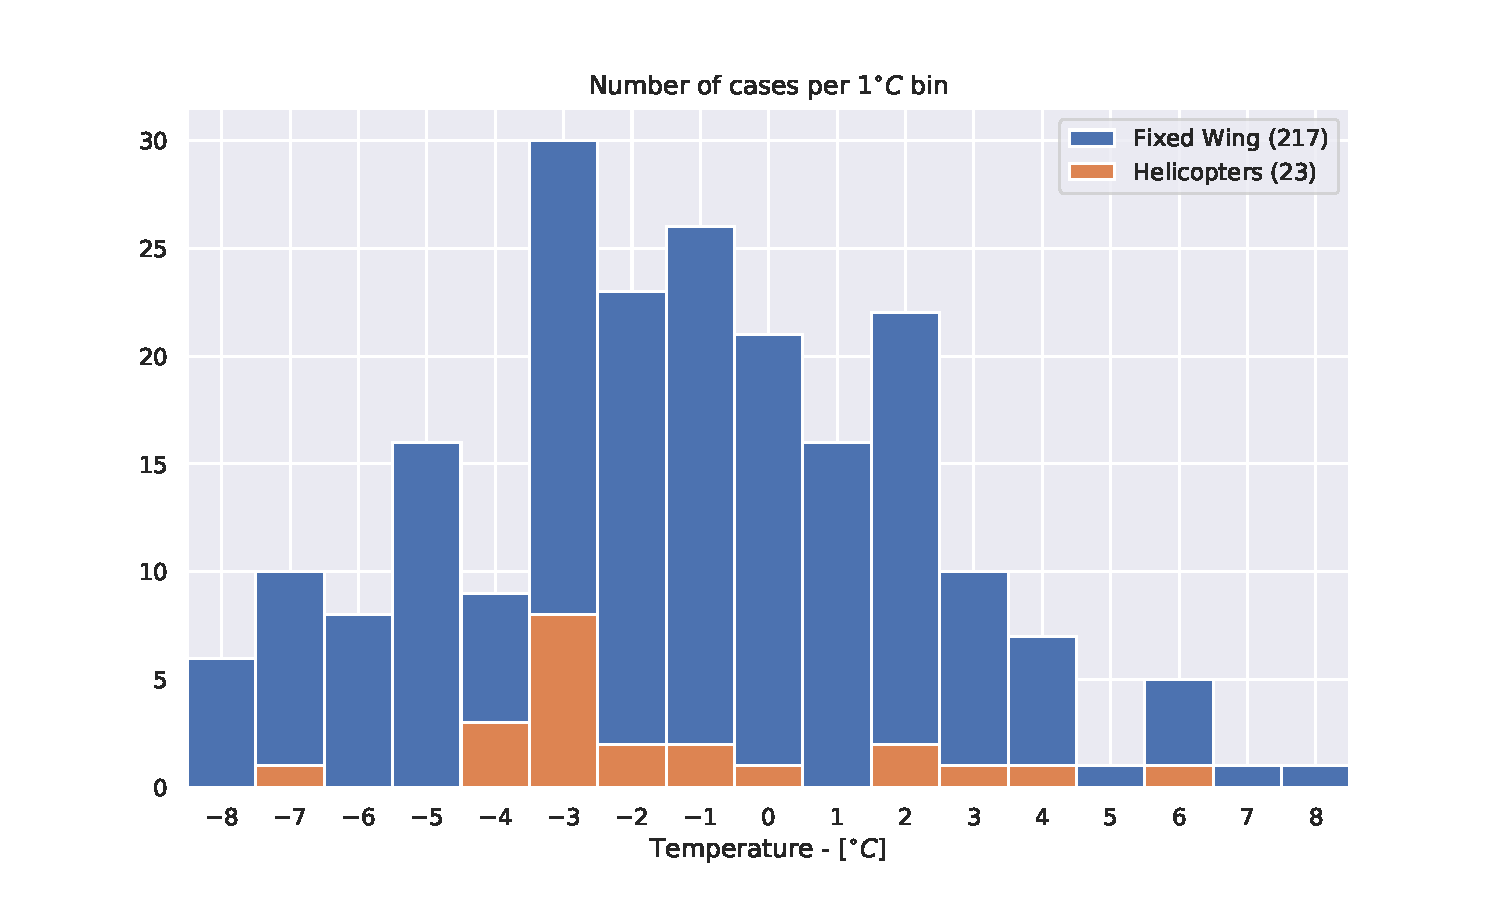
\includegraphics[width=\textwidth]{Figures/temperature.pdf}
    \caption{Temperature in fixed-wing and helicopter cases (interpolated from ERA5 pressure levels)}
    \label{fig:temperatureera5}
\end{figure}

\begin{figure}
    \centering
    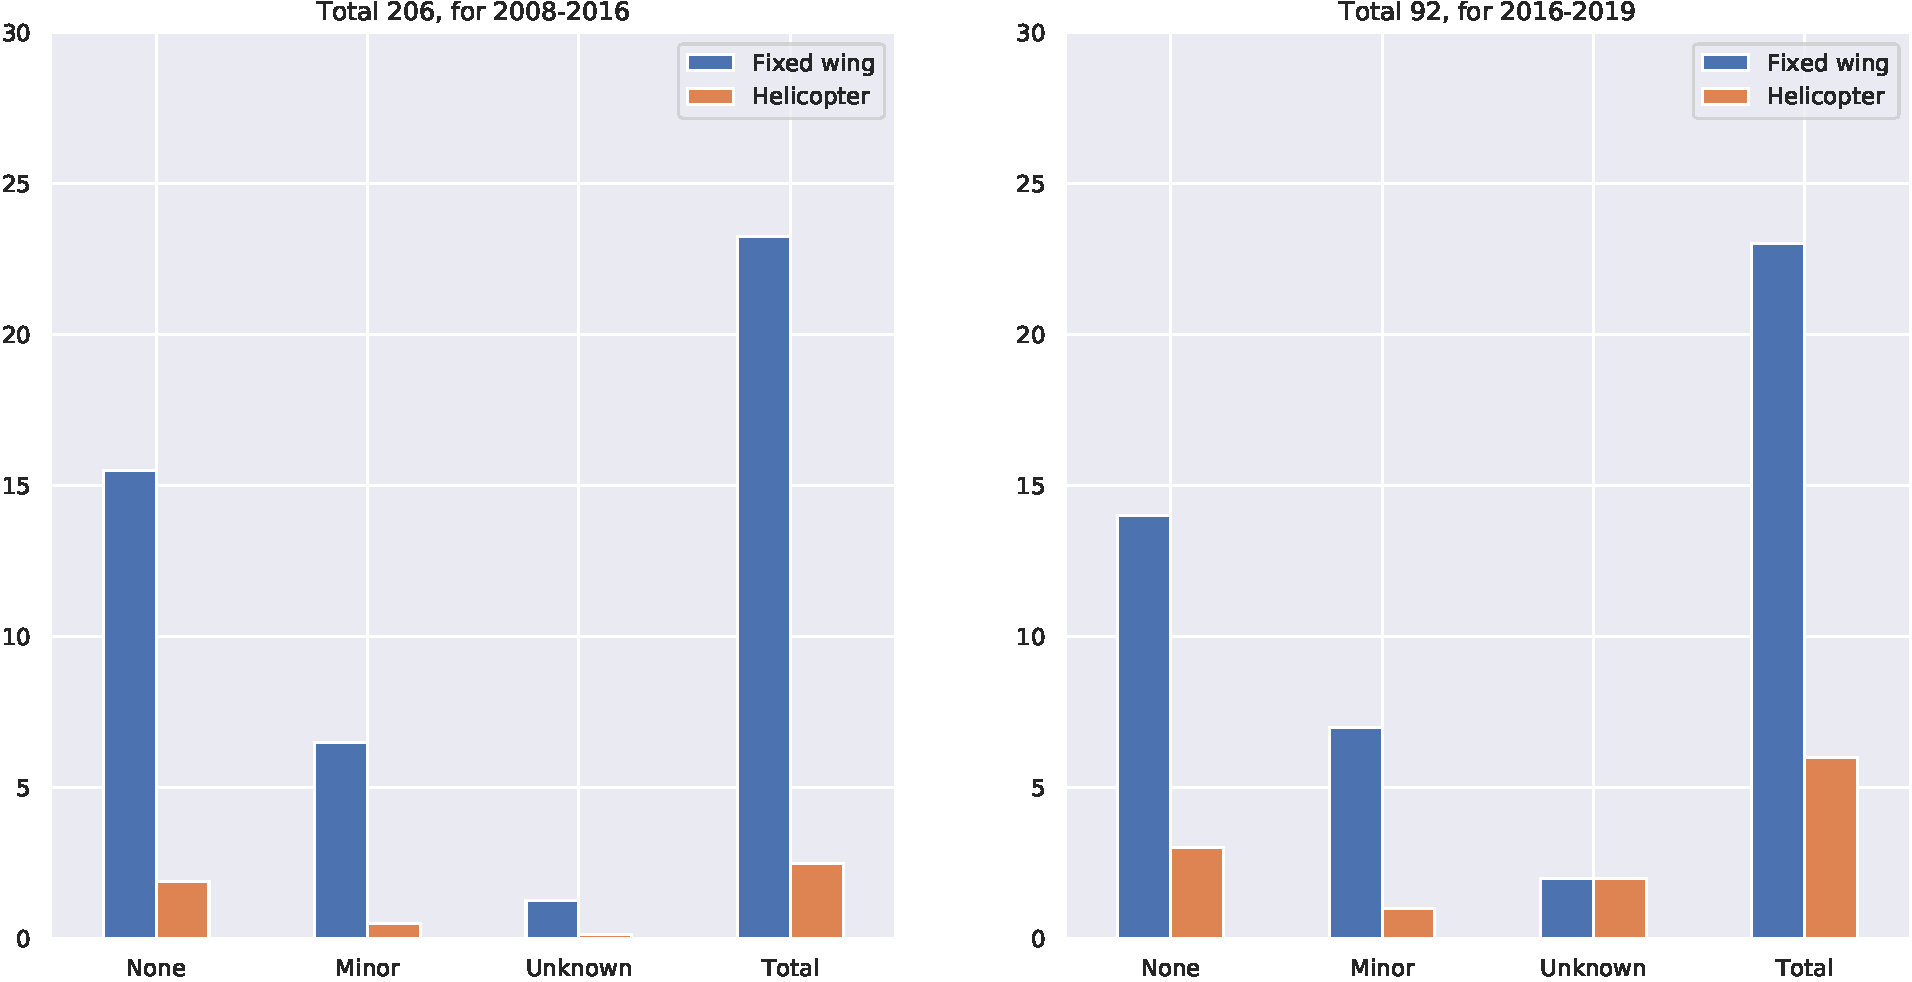
\includegraphics[width=\textwidth]{Figures/Casesperyear.pdf}
    \caption{Cases per year from the Avinor data set, delineated between cases before operational forecast was in place in the left figure, and after operational forecast was used in the right figure.}
    \label{fig:casesperyear}
\end{figure}

As discussed in Chapter \ref{ch:lightning}, there exists a body of research showing that the $0^{\circ}C$ isotherm in a cloud is related to winter- and \acrlong{htl}. Figure \ref{fig:yearlyvariation} shows that the Avinor data set has the same seasonal variation as these earlier studies, except for the additional case in May. This is presumably due to the Norwegian climate being generally colder than the British, which is where most of the earlier cases were from. Additionally, Figure \ref{fig:casesperyear} shows an increase in \acrshort{htl} cases after the introduction of the operational forecast, with a rate of 2 incidents per year before the forecast was introduced, to 5.5 incidents per year afterwards. Looking at the source data set, this seems to be more of a increase in reports from helicopter operators than an actual failing of the \acrshort{hti}. This is due to an increase in reports about incidents with no damage.

In contrast to the earlier research, the temperature found from ERA5 in Figure \ref{fig:temperatureera5} shows that the peak is situated around $-3^{\circ}C$ and not the $0^{\circ}C$ isotherm. This can either be attributed to a systematic error in pressure level interpolation (see Section \ref{sec:interpolation}), or due to operational procedures implemented due to \cite{lande1999}, which advises avoidance of the $0^{\circ}C$ isotherm when \acrshort{htl} is forecast or when flying inside of a cloud. Taking into account the \acrshort{fwtl} temperature in the same figure, there seems to be a $-1^{\circ}C$ shift from $0^{\circ}C$ since the peaks are at $-1^{\circ}C$ and $-3^{\circ}C$ compared to Figure \ref{fig:landetemp}. This also supports the previous statement about the effect of avoiding the $0^{\circ}C$ isotherm, as this is not a procedure followed by pilots flying fixed wing aircraft.

Figure \ref{fig:helisoner} shows the \acrshort{htl} incidents divided by the zones shown in Figure \ref{fig:Stationsmap}. It should be noted that there are no cases at Gardermoen, and only one case off the coast of Denmark in the Southern coast zone. The April peak is primarily contributed to by the North coast zone, which can be explained by the fact that the sea is still relatively warmer than the atmosphere during this time compared to the coast further south. This therefore supports earlier work in which it was proposed that cold air over warmer oceans caused convective systems to appear and be electrified. 

Figure \ref{fig:helivsfw} shows the same picture that \acrshort{htl} is a winter phenomenon and supports the claim in Section \ref{sec:fwtl} that \acrshort{fwtl} is an all-year phenomenon. The august peak in \acrshort{fwtl} can be explained by August being the month with the highest lightning activity in Norway. July also has some lightning activity, but commercial air travel is reduced compared to August. 

Figure \ref{fig:soner} shows that there is a geographical variation in cases, namely southern coast and Gardermoen primarily have cases during April-October, whereas the north, west and northwest are more represented during October-April. This shows a similar picture to that in \cite{koeltzow2018}: The Norwegian lightning climatology is primarily coastal in nature for winter lightning, and primarily inland for summer lightning. 


\begin{figure}[H]
    \centering
    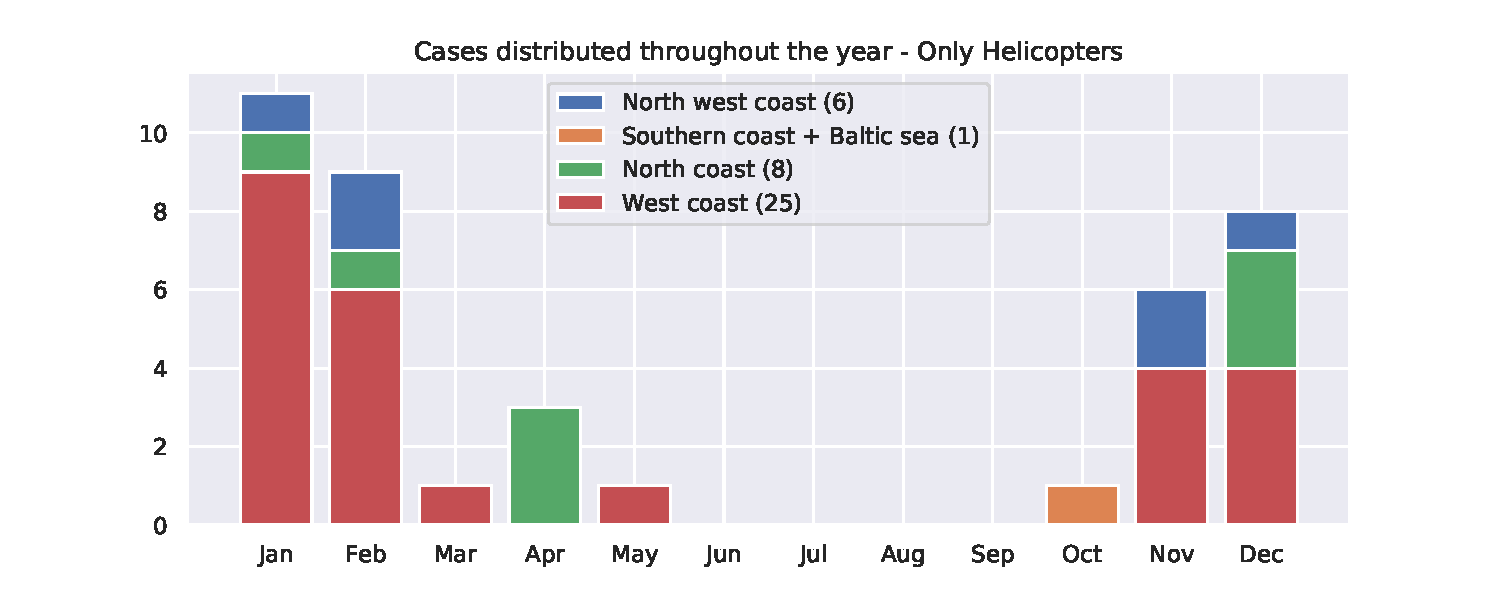
\includegraphics[width=\textwidth]{Figures/Helisoner.pdf}
    \caption{Zonal division of helicopter cases}
    \label{fig:helisoner}
\end{figure}

\begin{figure}[H]
    \begin{subfigure}{\textwidth}
    \centering
    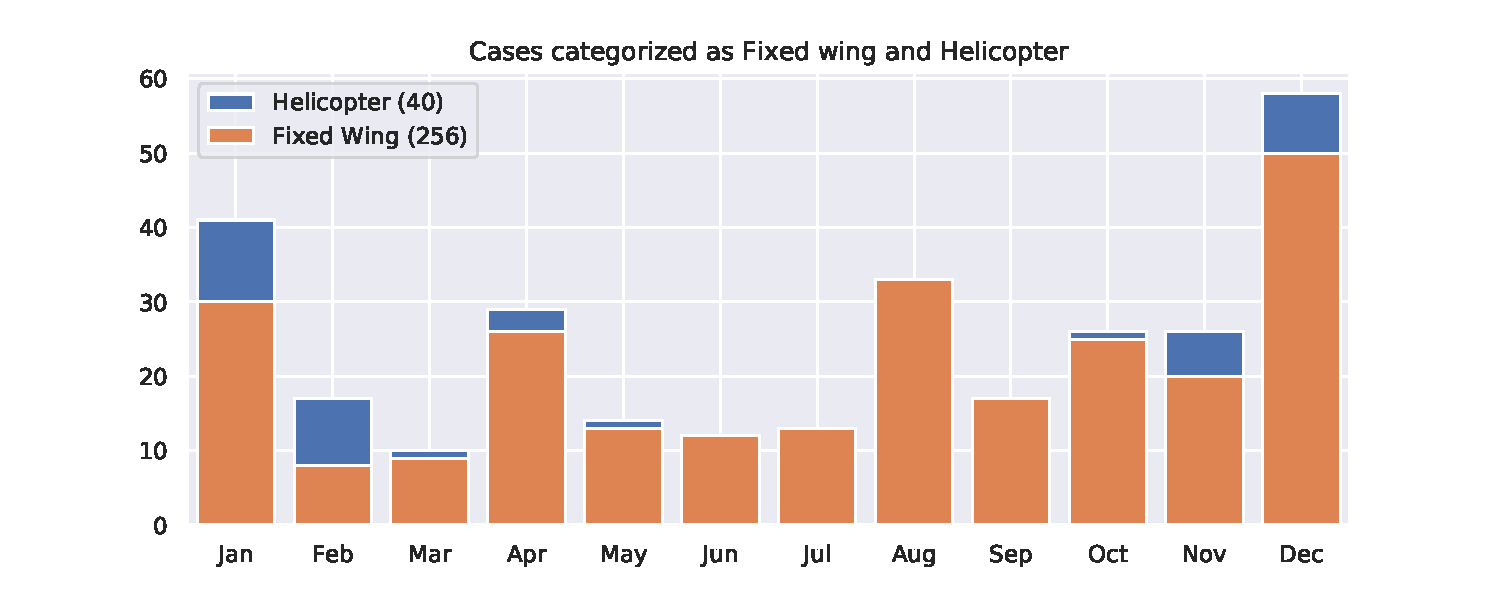
\includegraphics[width=\textwidth]{Figures/helivsfw.pdf}
    \caption{Yearly distribution of helicopter and fixed wing cases}
    \label{fig:helivsfw}
    \end{subfigure}
    
    \begin{subfigure}{\textwidth}
    \centering
    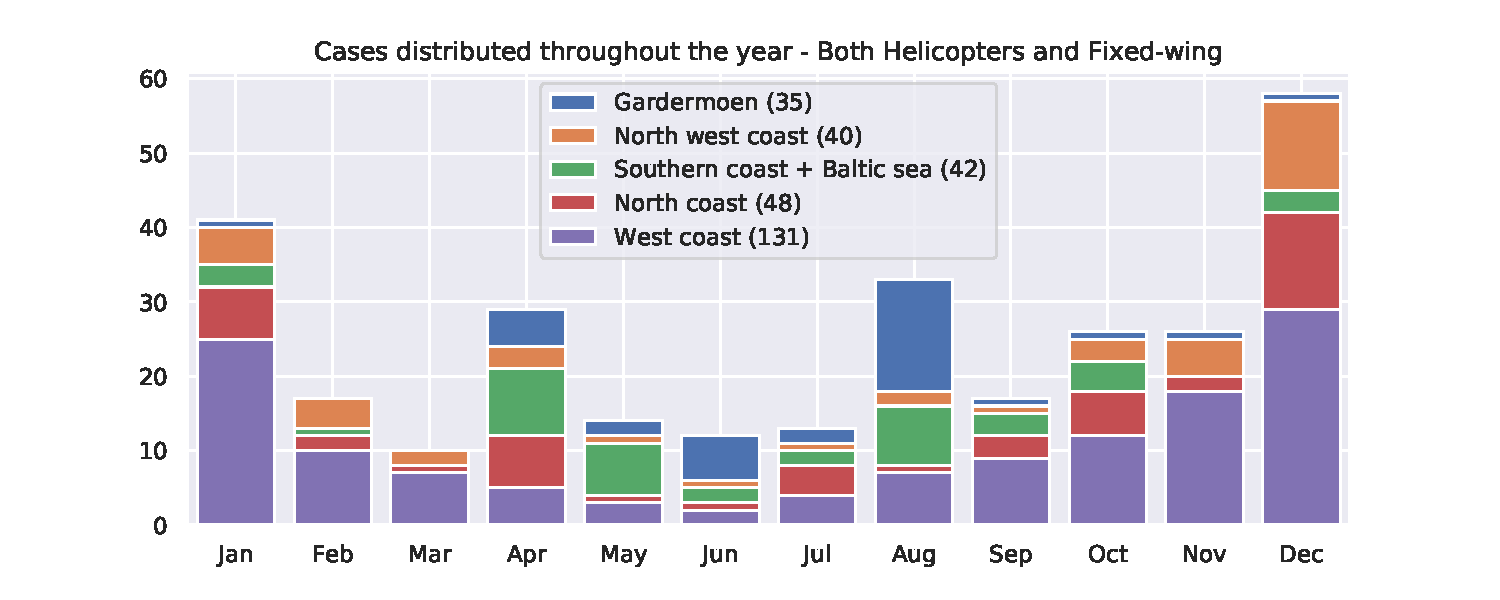
\includegraphics[width=\textwidth]{Figures/soner.pdf}
    \caption{Zonal division of helicopter and fixed wing cases, see Figure \ref{fig:helivsfw} for categorical distribution}
    \label{fig:soner}
    \end{subfigure}
\end{figure}

\section{Meteorological phenomena related to triggered lightning}

\subsection{METAR observations}

Figure \ref{fig:metarcases} shows the meteorological phenomena reported in the \acrshort{metar} report during triggered lightning incidents (both \acrshort{htl} and \acrshort{fwtl}). The helicopter cases show a high frequency (above 50 $\%$) for scattered, few and broken clouds, but zero of the cases had overcast conditions. Also found were showers in 20 $\%$ of the cases, and rain and/or snow was found in more than 20 $\%$ of the cases. Only 20 $\%$ of the cases had a report of cumulonimbus clouds. For the fixed wing, the cumulonimbus frequency is much higher (60 $\%$), and rain was in 40 $\%$ of the cases and snow in less than 5 $\%$. Showers were also often reported (60 $\%$). The fact that snow was less often reported for fixed wing compared to helicopter cases may be due to it being an all-year phenomenon such that snow was not observed at the ground during summer events. This, in turn, supports both \cite{lande1999} in that cumulonimbus was not \textit{always} observed during triggered lightning incidents, and the choice to include maximum cloud cover minus minimum cloud cover since almost none of the cases show overcast conditions.

\begin{figure}[H]
    \centering
    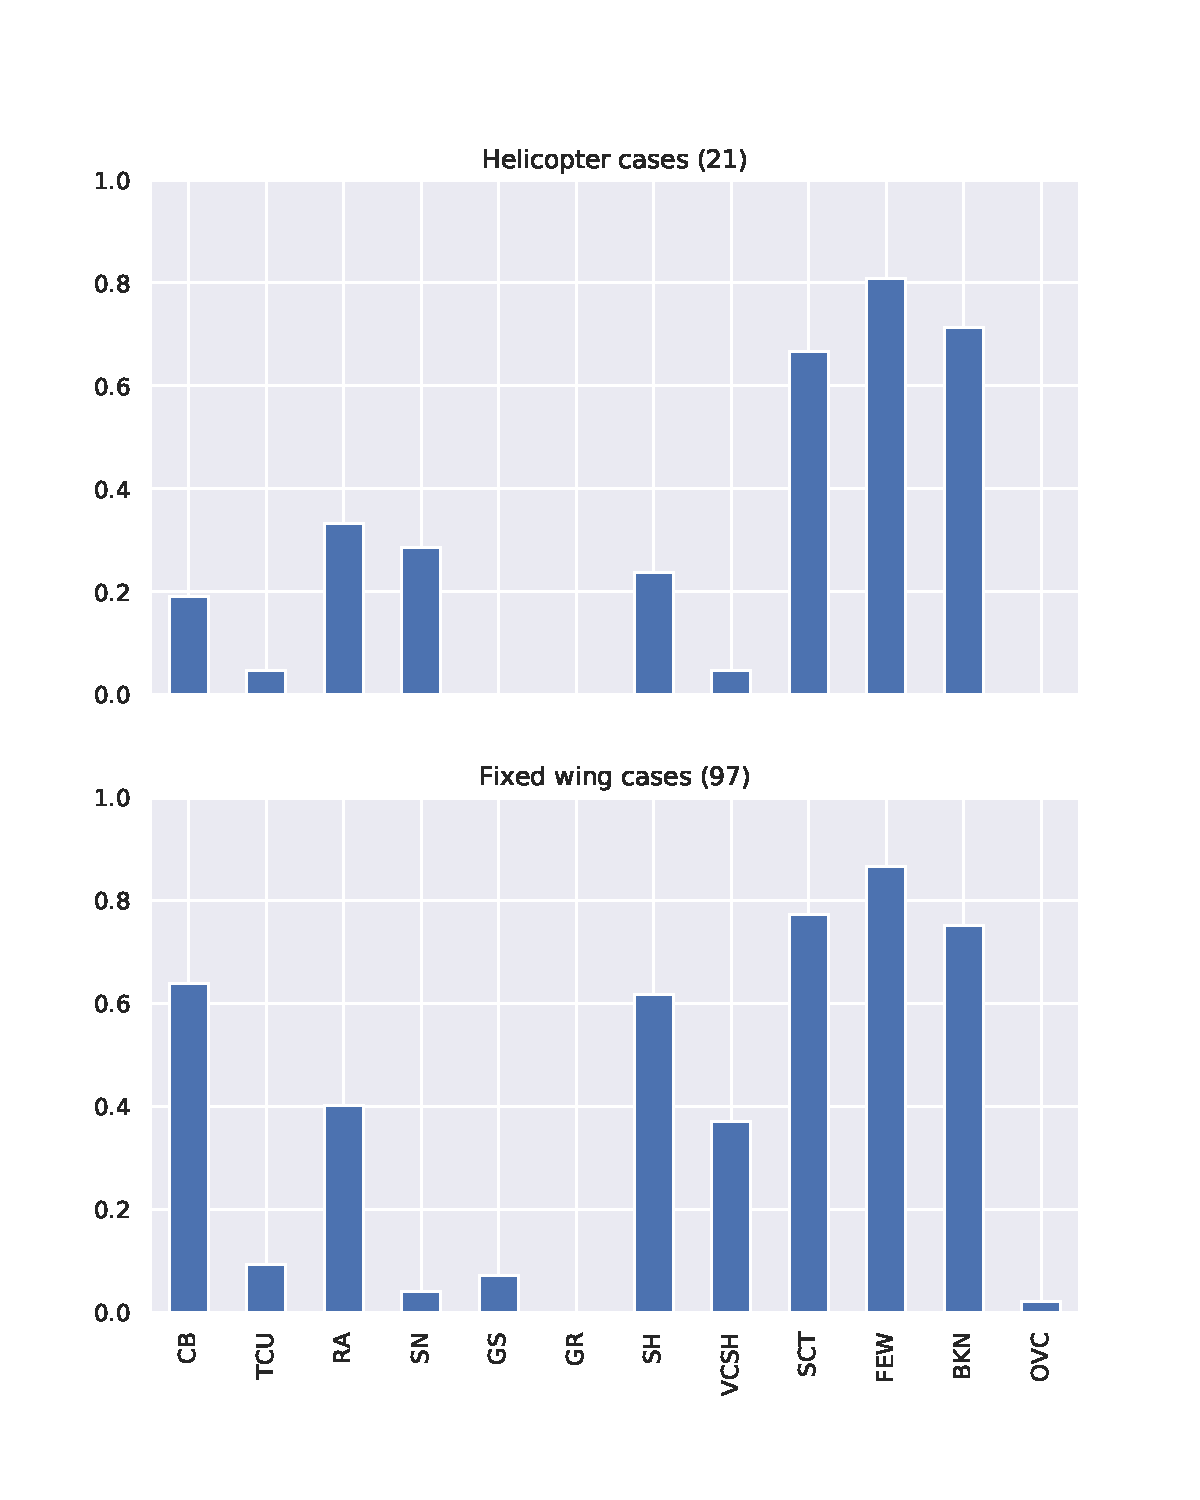
\includegraphics[width=\textwidth]{Figures/METARcases.pdf}
    \caption{Frequency of different categories of \acrshort{metar}-phenomenon for Helicopter and Fixed wing cases, included are only cases where airport had a \acrshort{metar}-report that was taken by a non-automatic system. Note that SH also include VCSH}
    \label{fig:metarcases}
\end{figure}

\begin{figure}[H]
    \centering
    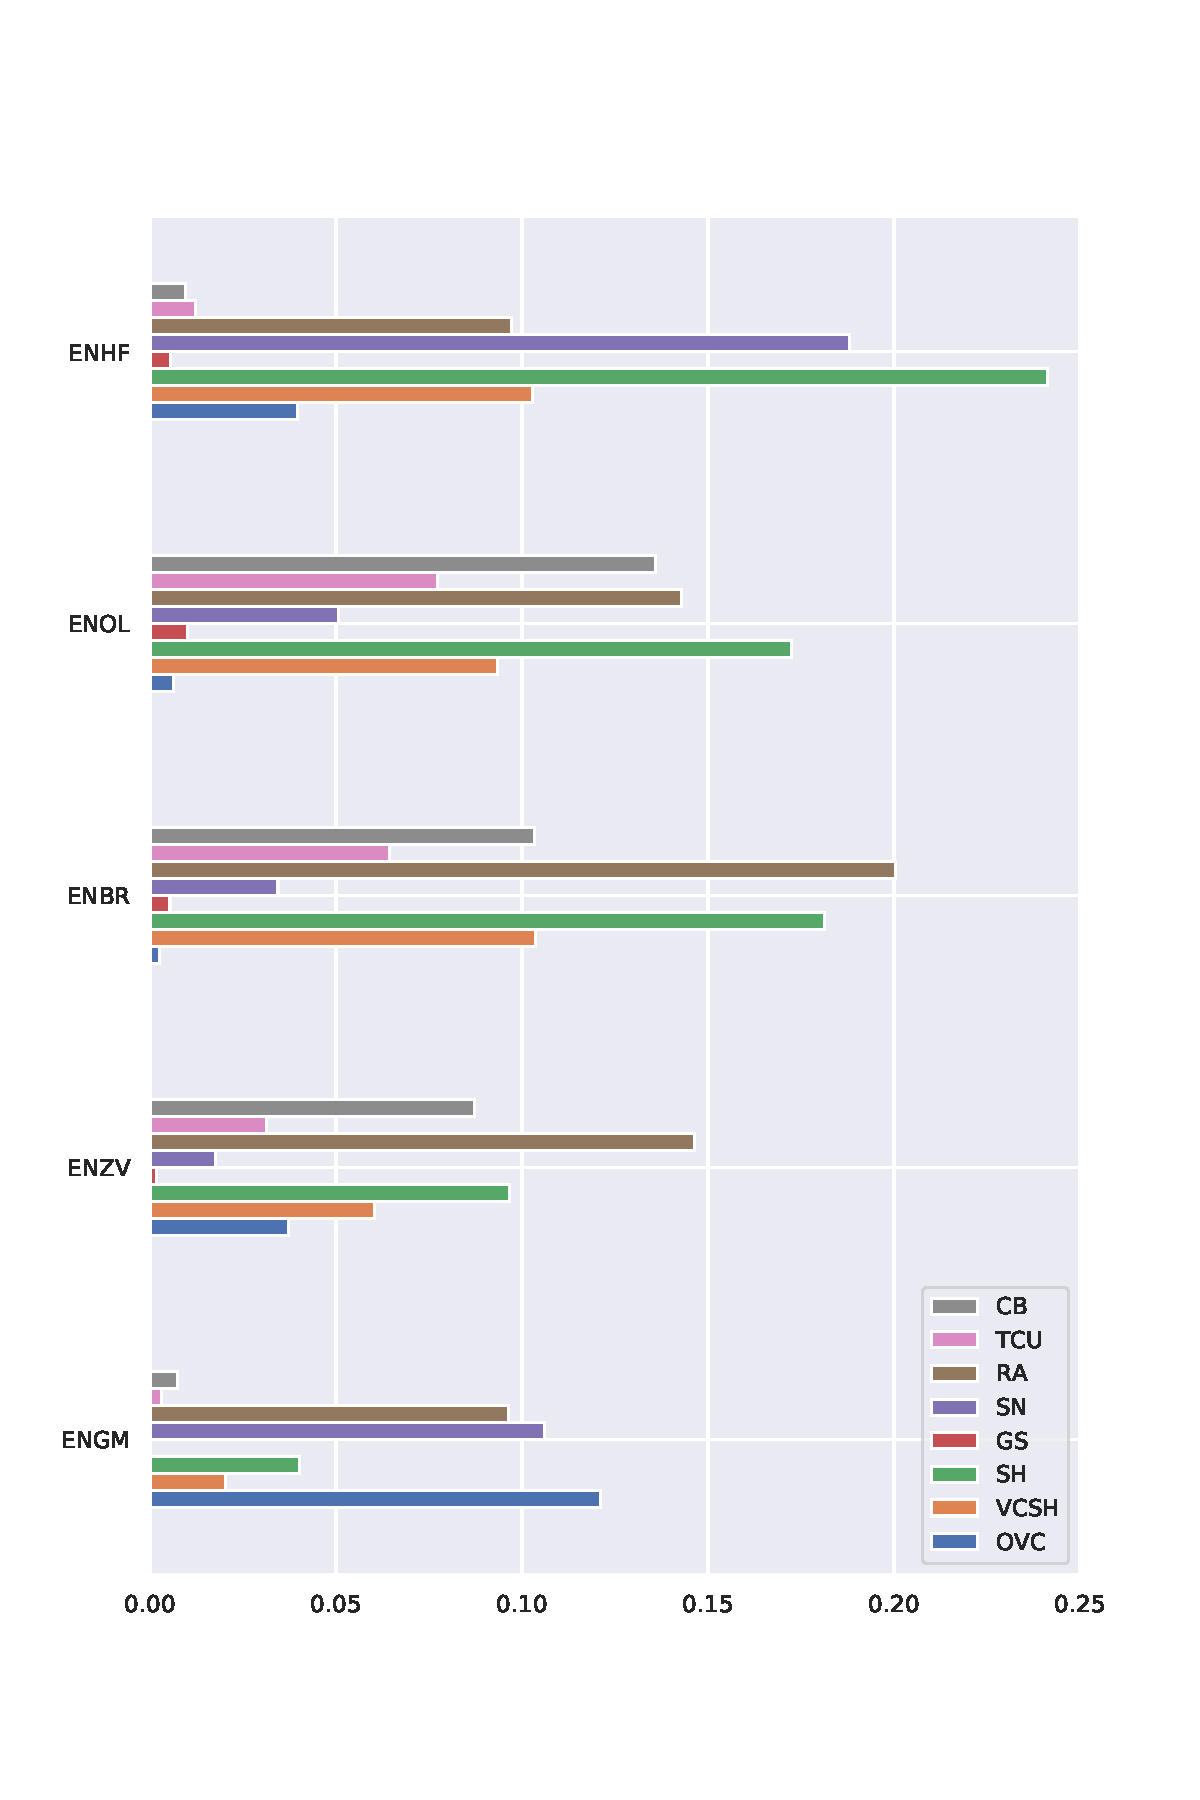
\includegraphics[width=.9\textwidth]{Figures/METAR_airports.pdf}
    \caption{Percentage of \acrshort{metar}-reports involving at least one of the meteorological phenomena at Hammerfest, Ørlandet, Flesland, Sola, and Gardermoen airports. Selection is based on geographical variation and representation.}
    \label{fig:metarclimat}
\end{figure}


To investigate the parameters used in the operational \acrshort{hti} forecast, composites have been created for the cases from the Avinor data set. The parameters studied are temperature, vertical velocity, precipitation and cloud cover. Cloud cover did not show any clear signal due to ERA5 horizontal scale, and therefore was moved to Appendix \ref{app:A}. Also studied is the general circulation during these cases, by looking at the composite of the mean sea level pressure. 

\subsection{Temperature during triggered lightning events} \label{sec:compositesera5}
Shown in Figure \ref{fig:tempzones} are temperature composites divided into the geographical zones described in Appendix \ref{app:B}. The figure reveals that for the different geographic zones, the average temperature in the composites are around -3 to 0$^{\circ}C$. This is in accordance with previous findings that \acrshort{htl} happens at temperatures right below or at 0$^{\circ}C$. One also sees that grouping of the cases leads to a reduction in the standard deviation along each zone's coast, except for the North zone. This hints to that these temperatures are closely related, but North zone should ideally be divided into finer zones. (This would, however, be less robust due to the North zone only containing 40 cases.)

Figure \ref{fig:tempairports} shows that the temperatures at Flesland and Sola are, as expected, around 0 to -1$^{\circ}C$, and here the variation in temperature is much lower as seen in the respective standard deviation plots. The standard deviation is lowest in Flesland, but this is to be expected, since there are double the amount of cases at Flesland than Sola. Looking, though, at Figure \ref{fig:ENGMTemperature}, one sees that Gardermoen airport has a much warmer situation at around +2$^{\circ}C$. Here, the standard deviation also is higher. This coincides with the variation shown in Figure \ref{fig:temperatureera5}. 

\subsection{Typical pressure pattern during triggered lightning events}\label{sec:pressure}
Figure \ref{fig:tempzones} contains, in addition to temperature, composites of pressure during triggered lightning events. The general circulation from these pressure systems seems to tend toward geostrophic wind directed toward the coast. Notable exception is the South zone, which does not have a clear low pressure system in the ocean, but the standard deviation hints to a lot of variation over the ocean. The geostrophic winds for the remaining zones also would be coming from colder areas, i.e. Iceland and the Arctic. This would lead to cold air being blown over the relatively warm North Atlantic Current, as discussed in Section \ref{sec:winter lightning}, as a precursor for convection and lightning activity. The pressure in Figure \ref{fig:tempairports} shows the same picture for both Flesland and Sola airports, being dominated by low pressure systems situated in the Norwegian Sea, such that the geostrophic wind would be directed inland toward the airports. The convection observed here may be a result of topography and surface roughness changing when moving from ocean to land. Since the land does not dissipate the kinetic energy in form of waves, the energy leads to more turbulence in the air, causing local convection. This suggests that wind incident on land is present in most cases of triggered lightning events at the coast of Norway. 

However, Gardermoen being located inland does not see this roughness effect. This suggests that incidents at Gardermoen are instead related to local convective systems seen in the summertime. This explains why Gardermoen airport's pressure situation is "normal" during triggered lightning events, since the incidents are related to local convective systems, rather than bigger circulation causing local convection. The standard deviation shows the same picture in that the pressure does not have a large standard deviation.

\begin{figure}[H]
\begin{subfigure}[b]{0.49\textwidth}
    \centering
    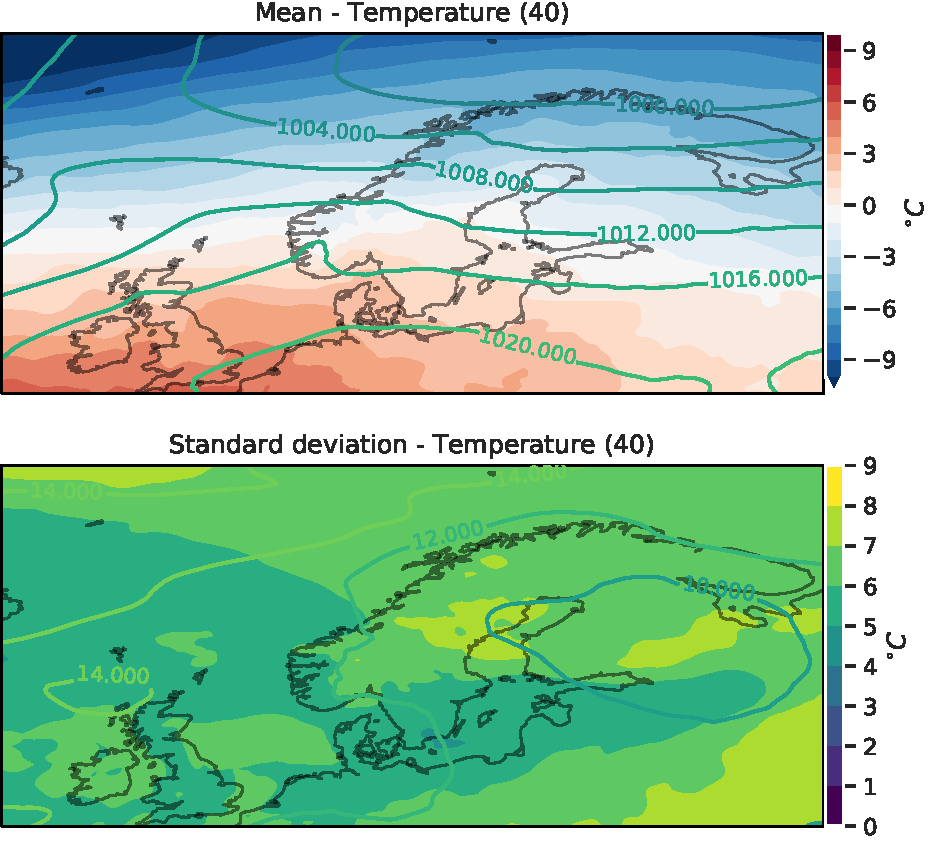
\includegraphics[width=\textwidth]{Figures/TempNord.pdf}
    \caption{Temperature for cases in North zone.}
    \label{fig:NordTemperature}
\end{subfigure}
\begin{subfigure}[b]{0.49\textwidth}
    \centering
    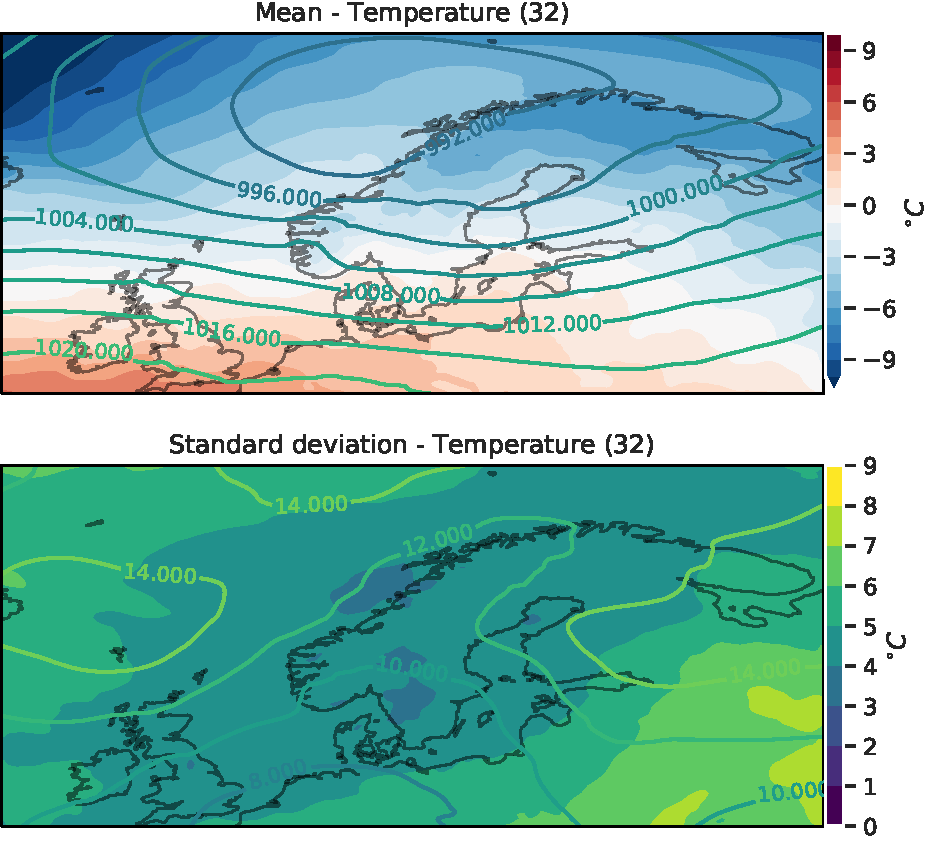
\includegraphics[width=\textwidth]{Figures/TempNordvest.pdf}
    \caption{Temperature for cases in Northwest zone.}
    \label{fig:NordWestTemperature}
\end{subfigure}
\begin{subfigure}[b]{0.49\textwidth}
    \centering
    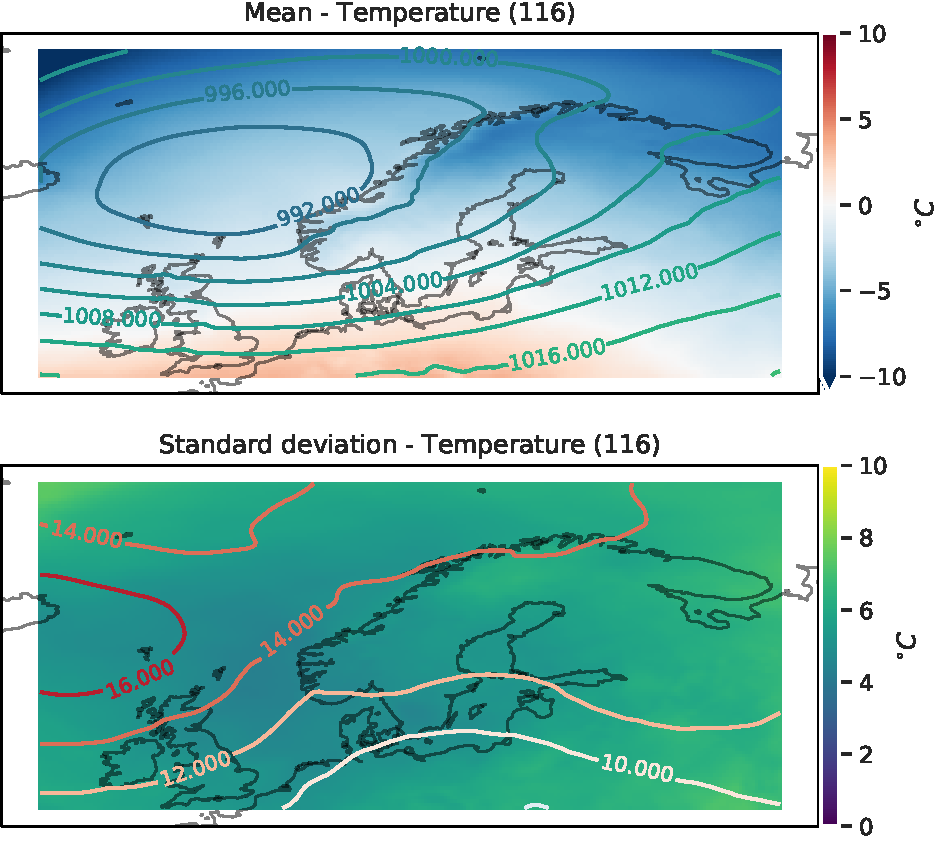
\includegraphics[width=\textwidth]{Figures/TempVest.pdf}
    \caption{Temperature for cases in West zone.}
    \label{fig:WestTemperature}
\end{subfigure}
\begin{subfigure}[b]{0.49\textwidth}
    \centering
    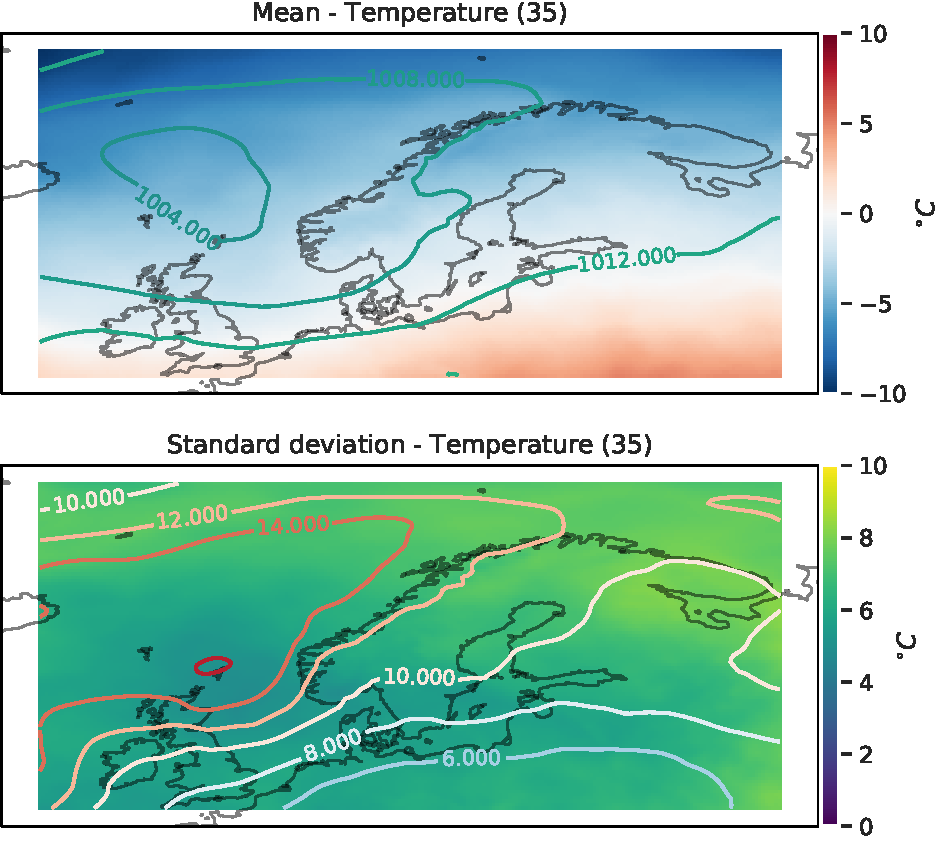
\includegraphics[width=\textwidth]{Figures/TempSor.pdf}
    \caption{Temperature for cases in South zone.}
    \label{fig:SouthTemperature}
\end{subfigure}
\caption{Temperature composites for both \acrshort{htl} and \acrshort{fwtl} cases in different geographical zones. Included are only cases for which height information was provided in the Avinor data set. The temperature was found by interpolating to the correct height as described in Section \ref{sec:interpolation}}
\label{fig:tempzones}
\end{figure}

\begin{figure}[H]
     \centering
     \begin{subfigure}[b]{0.49\textwidth}
         \centering
         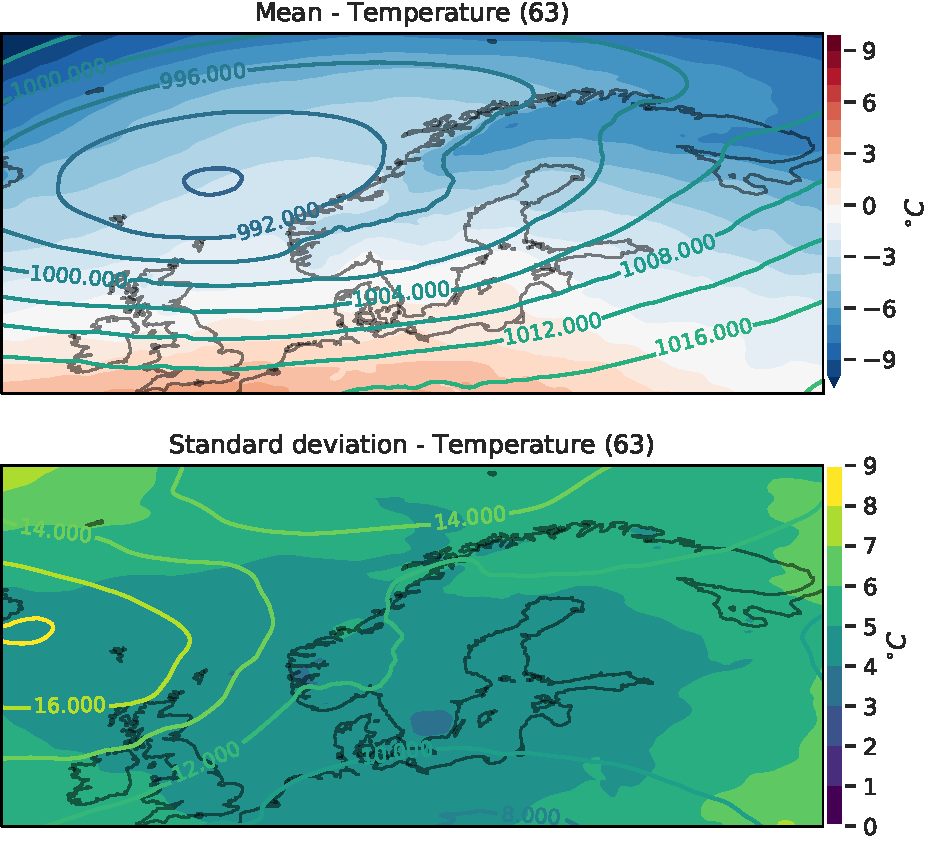
\includegraphics[width=\textwidth]{Figures/TempENBR.pdf}
         \caption{Temperature for cases at Flesland airport.}
         \label{fig:ENBRTemperature}
     \end{subfigure}
     \hfill
     \begin{subfigure}[b]{0.49\textwidth}
         \centering
         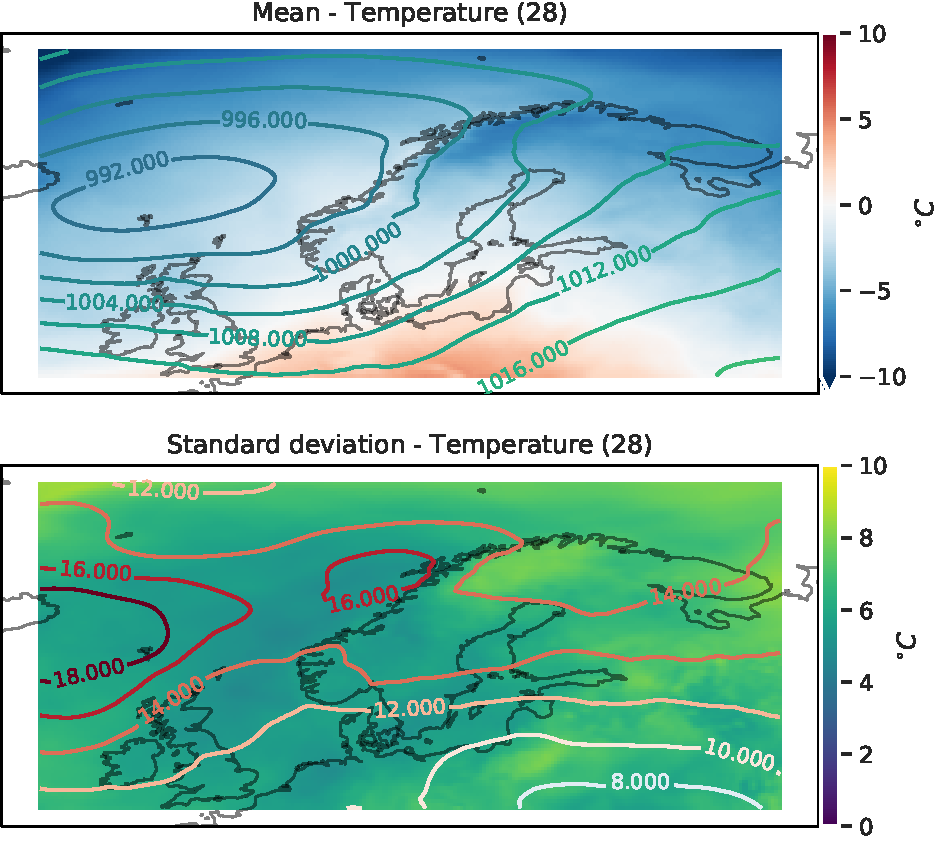
\includegraphics[width=\textwidth]{Figures/TempENZV.pdf}
         \caption{Temperature for cases at Sola airport.}
         \label{fig:ENZVTemperature}
     \end{subfigure}

    \begin{subfigure}[b]{0.5\textwidth}
    \centering
    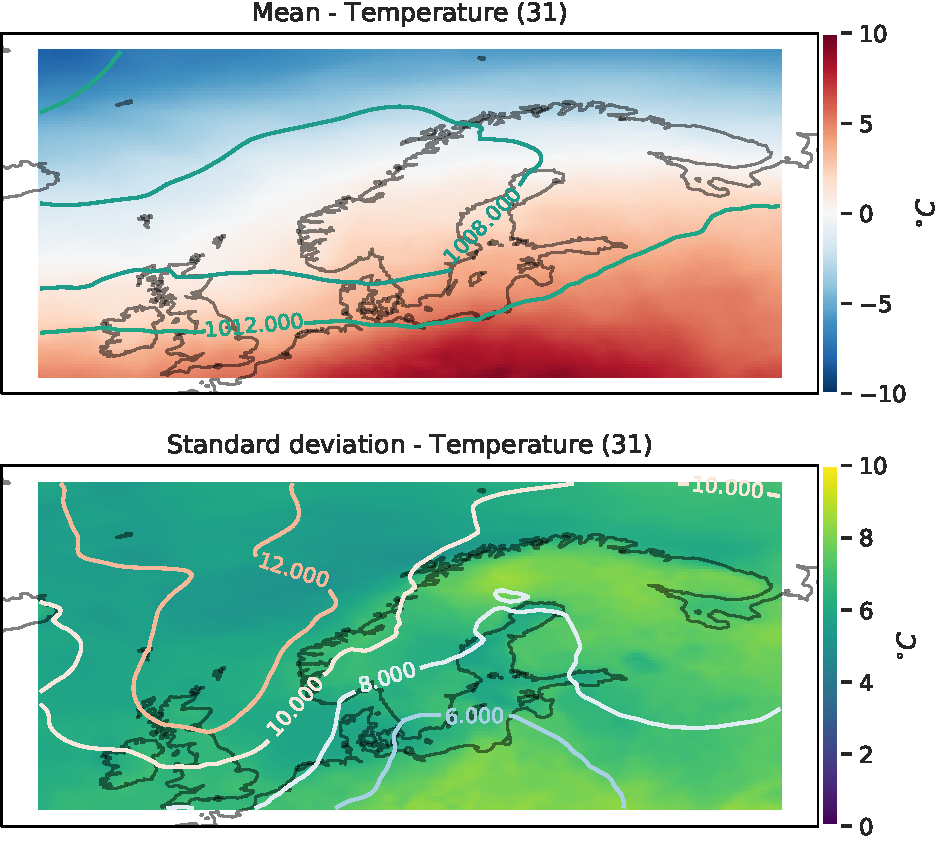
\includegraphics[width=\textwidth]{Figures/TempENGM.pdf}
    \caption{Temperature for cases in Gardermoen zone.}
    \label{fig:ENGMTemperature}
\end{subfigure}
\caption{Same as Figure \ref{fig:tempzones}, but for only the biggest airports. }
\label{fig:tempairports}
\end{figure}

\subsection{Vertical velocity during triggered lightning events}\label{sec:verticalvelocity}

Figure \ref{fig:verticalzones} shows vertical velocity composites for the different geographic zones. It should be noted that the color bar is inverted, such that red is negative and blue is positive. This is done due to the units being Pa/s, so that negative values infers upward velocity and positive downward velocity. One can see a clear trend among the coastal zones (north, northwest and west) that there is upward vertical velocity related to the cases. There is also a somewhat high standard deviation in these same zones, but this could be related to \textit{placing} of the upward velocity systems in the model. Looking at Figure \ref{fig:verticalairports}, one sees the same for both Flesland and Sola: A clear vertical velocity in the composite, but some higher standard deviation in the Sola case. (Again, presumably because of the lower number of cases.) There is a very weak vertical velocity for the Gardermoen case. This can be explained by Gardermoen predominantly being subject to summer lightning, which is due to local convective areas and may not be correctly resolved in the coarse horizontal grid of ERA5. 

\begin{figure}[H]
\begin{subfigure}[b]{0.49\textwidth}
    \centering
    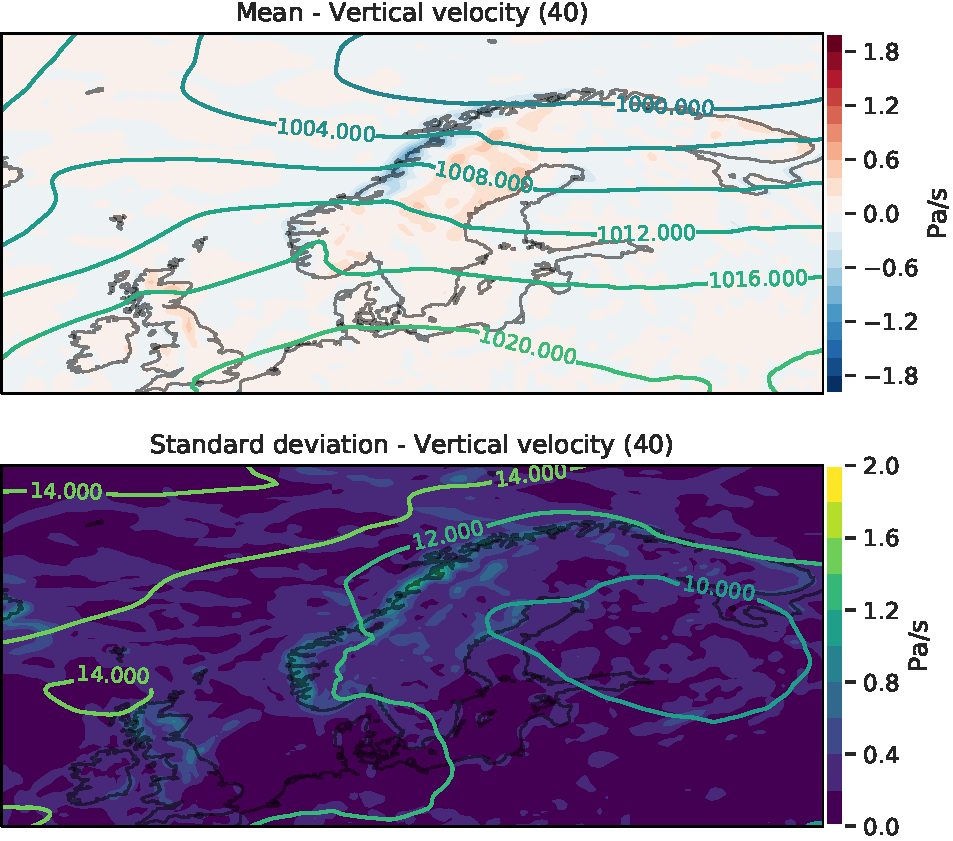
\includegraphics[width=\textwidth]{Figures/WNord.pdf}
    \caption{Vertical velocity for cases in North zone.}
    \label{fig:NordW}
\end{subfigure}
\begin{subfigure}[b]{0.49\textwidth}
    \centering
    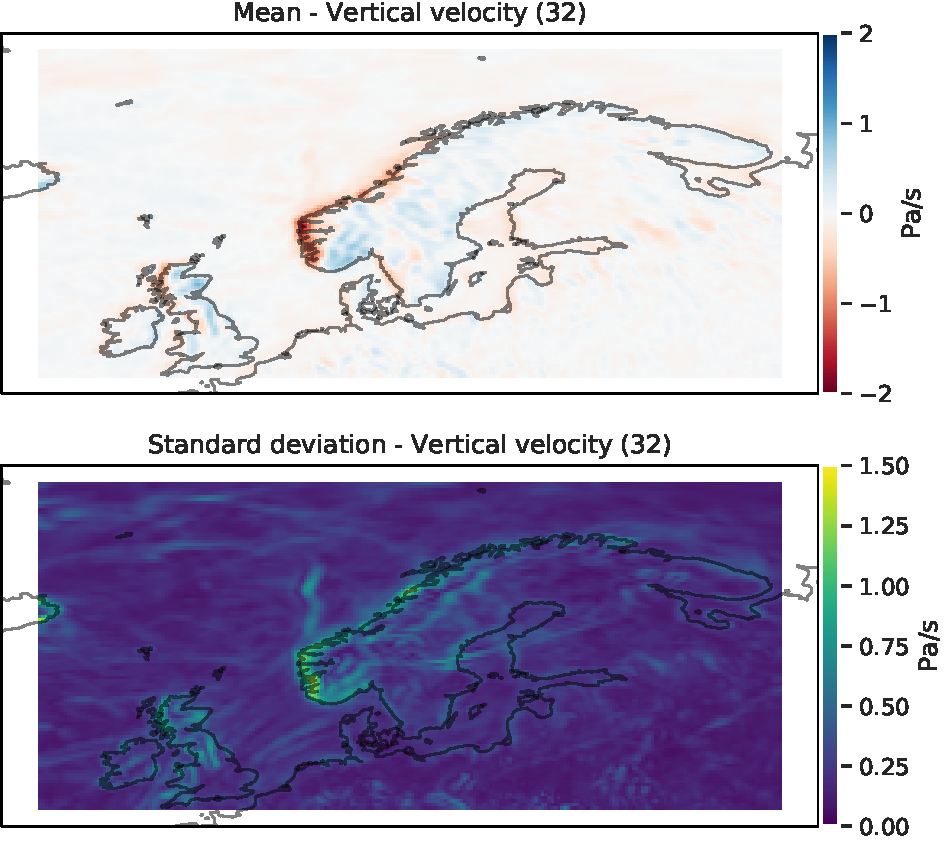
\includegraphics[width=\textwidth]{Figures/WNordvest.pdf}
    \caption{Vertical velocity  for cases in Northwest zone.}
    \label{fig:NordWestW}
\end{subfigure}
\begin{subfigure}[b]{0.49\textwidth}
    \centering
    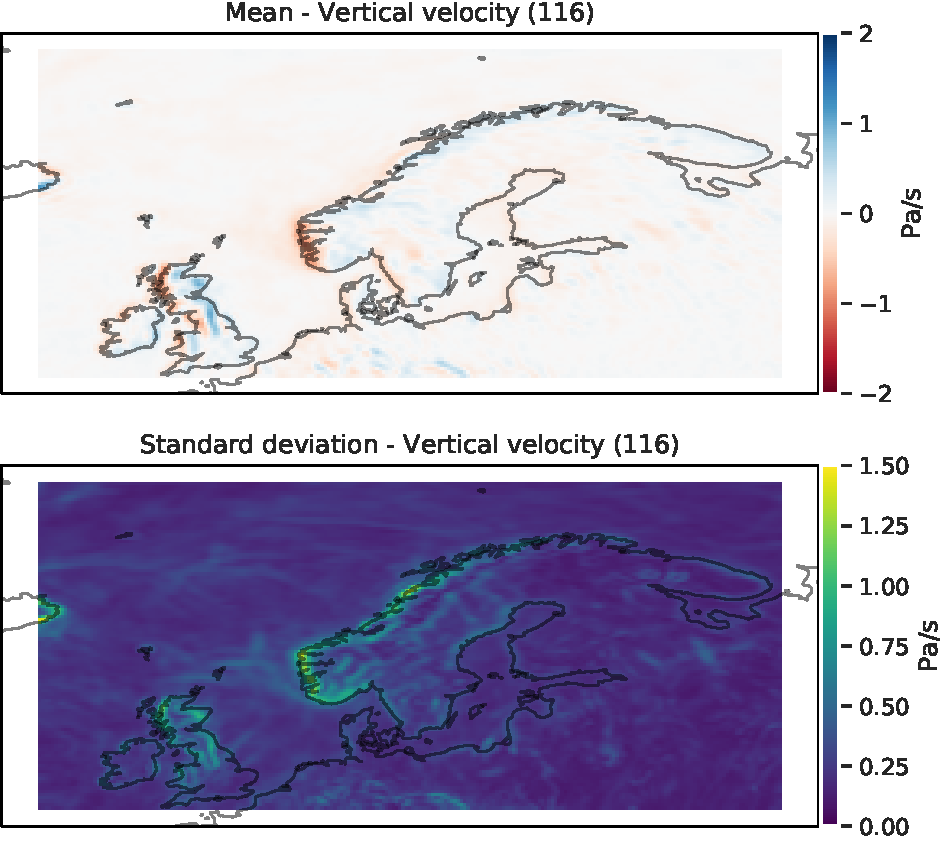
\includegraphics[width=\textwidth]{Figures/WVest.pdf}
    \caption{Vertical velocity  for cases in West zone.}
    \label{fig:WestW}
\end{subfigure}
\begin{subfigure}[b]{0.49\textwidth}
    \centering
    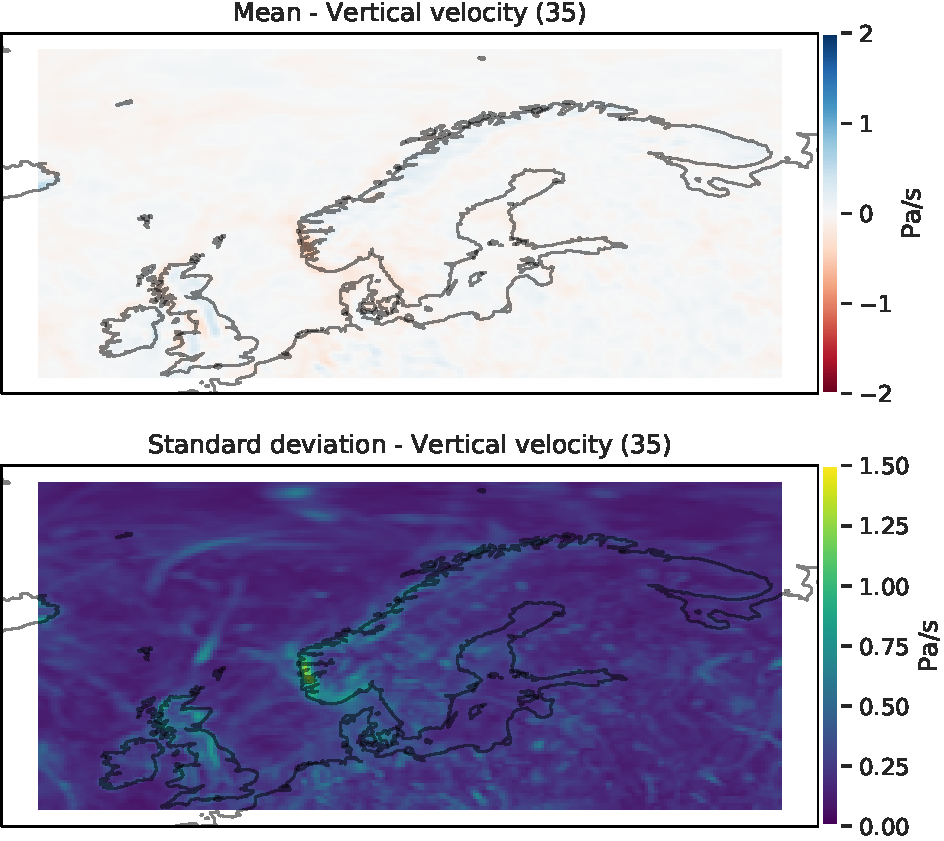
\includegraphics[width=\textwidth]{Figures/WSor.pdf}
    \caption{Vertical velocity  for cases in South zone.}
    \label{fig:SouthW}
\end{subfigure}
\caption{Vertical velocity composites for both \acrshort{htl} and \acrshort{fwtl} cases in different geographical zones. Included are only cases for which height information was provided in the Avinor data set. The velocity was found by interpolating to the correct height as described in Section \ref{sec:interpolation}}
\label{fig:verticalzones}
\end{figure}

\begin{figure}[H]
     \centering
     \begin{subfigure}[b]{0.49\textwidth}
         \centering
         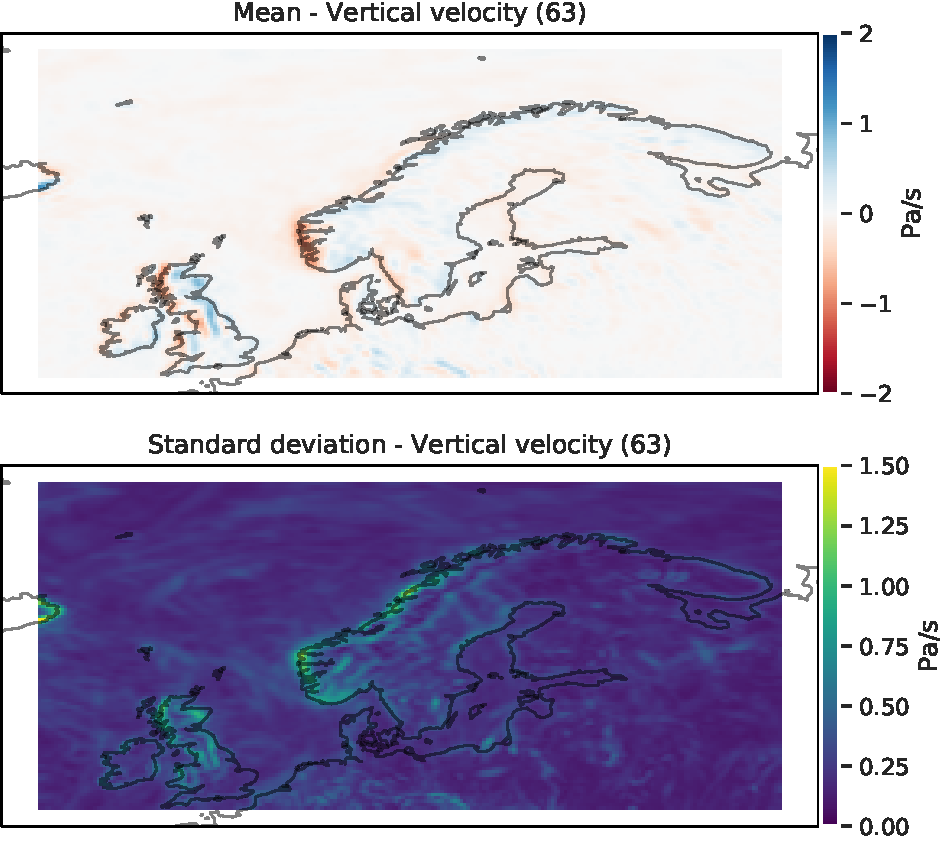
\includegraphics[width=\textwidth]{Figures/WENBR.pdf}
         \caption{Vertical velocity for cases at Flesland}
         \label{fig:ENBRW}
     \end{subfigure}
     \hfill
     \begin{subfigure}[b]{0.49\textwidth}
         \centering
         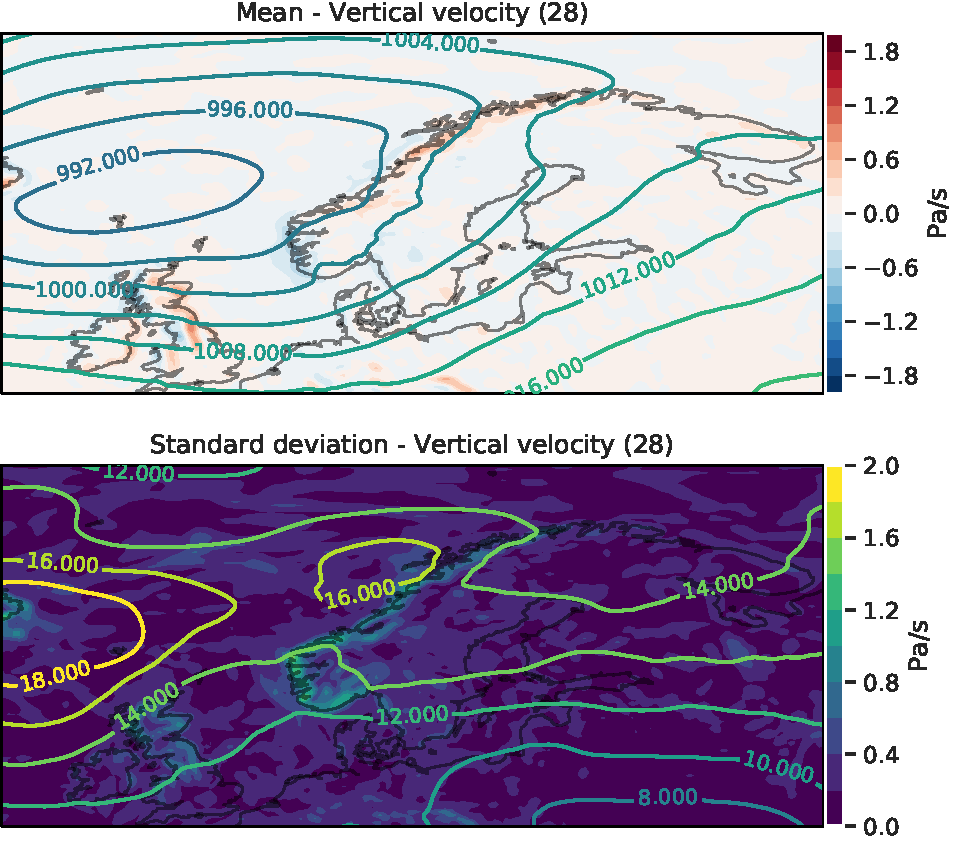
\includegraphics[width=\textwidth]{Figures/WENZV.pdf}
         \caption{Vertical velocity for cases at Sola}
         \label{fig:ENZVW}
     \end{subfigure}
    \begin{subfigure}[b]{0.5\textwidth}
    \centering
    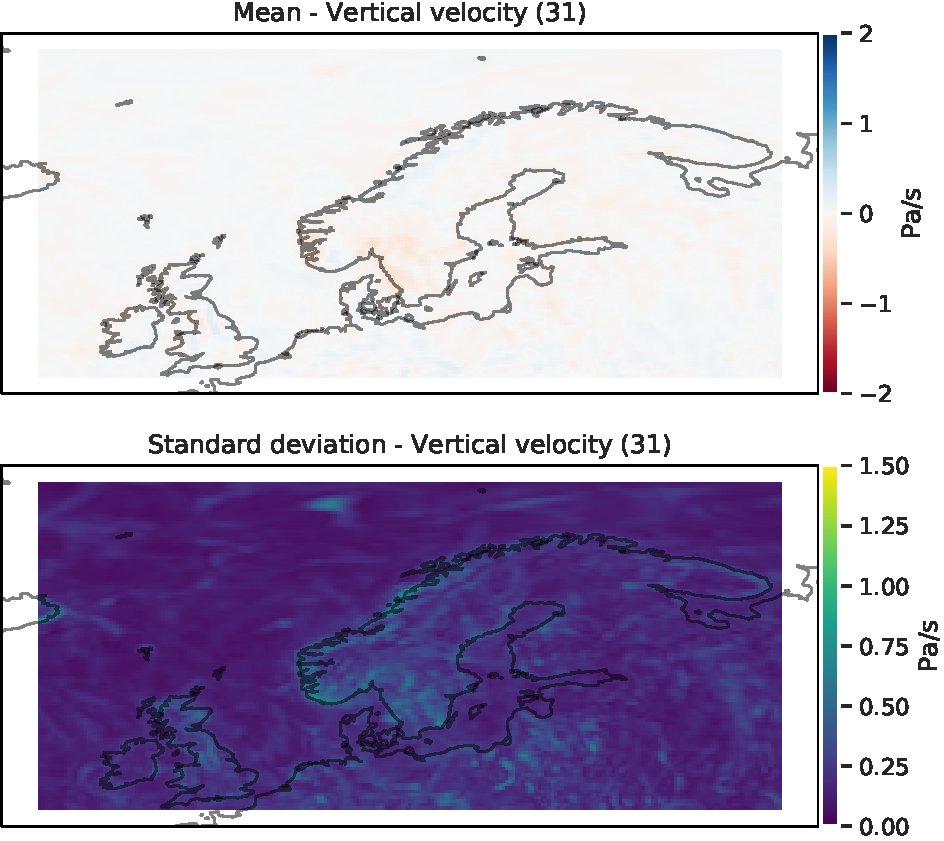
\includegraphics[width=\textwidth]{Figures/WENGM.pdf}
    \caption{Vertical velocity for cases in Gardermoen zone.}
    \label{fig:ENGMW}
\end{subfigure}
\caption{Same as Figure \ref{fig:verticalzones}, but for only the biggest airports.}
\label{fig:verticalairports}
\end{figure}


\subsection{Different types of precipitation for triggered lightning events}
The ERA5 reanalysis model differentiates between convective precipitation arising from the convection scheme in the integrated forecasting system and large scale precipitation arising from the cloud scheme in the integrated forecasting system. To investigate the atmospheric conditions, this thesis divides into these two different categories of precipitation to distinguish between large scale and locally caused precipitation.

\subsubsection{Large scale precipitation}
Figure \ref{fig:largescalezones} shows no clear sign of large scale precipitation being present anywhere but the west coast of Norway. However, for \textit{all} the composites (all zones), only the west coast has substantial amounts of large scale precipitation. This is further reinforced when looking at the case for Flesland and Sola in Figure \ref{fig:largescaleairports}. Again, Gardermoen sticks out due to not having any clear sign of large scale precipitation neither at the west coast nor around Gardermoen. This can again be explained by Gardermoen predominantly having triggered lightning events during summertime.

\begin{figure}[H]
\begin{subfigure}[b]{0.49\textwidth}
    \centering
    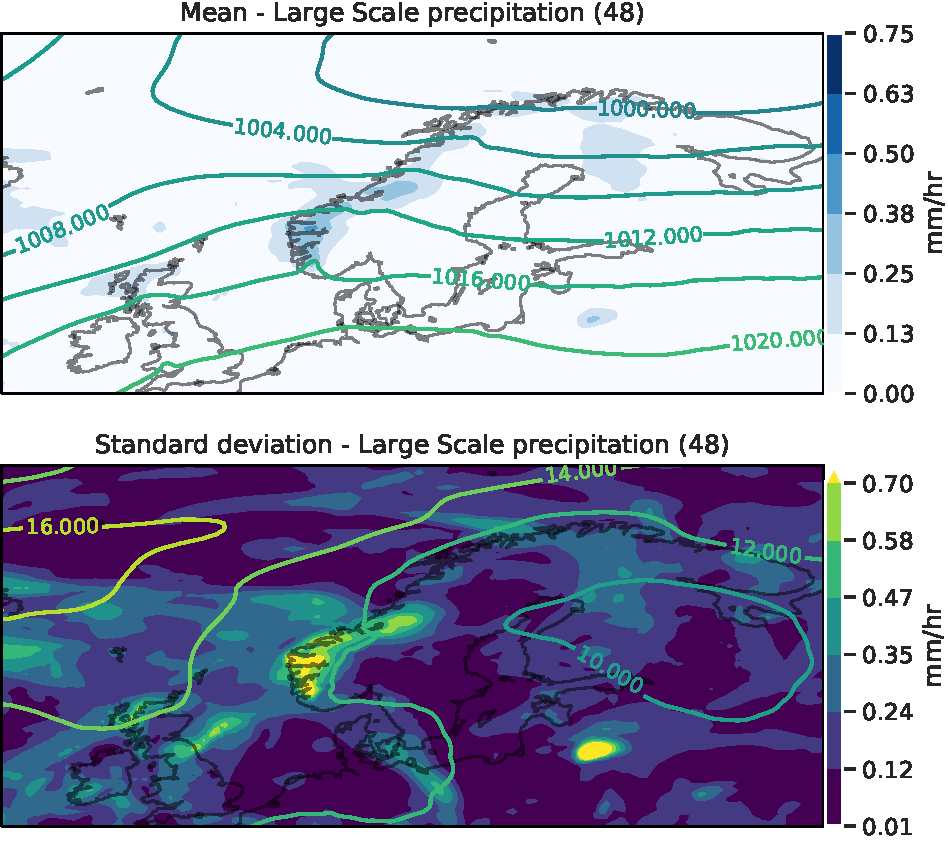
\includegraphics[width=\textwidth]{Figures/lsPNord.pdf}
    \caption{Large scale for cases in North zone.}
    \label{fig:NordlsP}
\end{subfigure}
\begin{subfigure}[b]{0.49\textwidth}
    \centering
    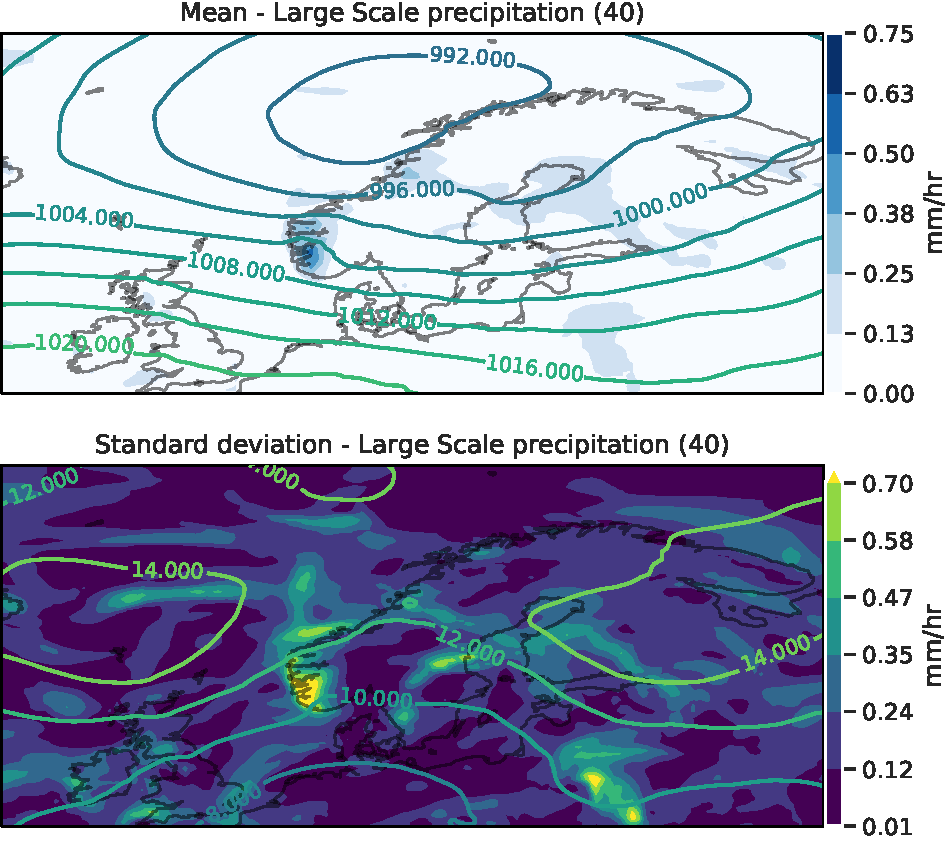
\includegraphics[width=\textwidth]{Figures/lsPNordvest.pdf}
    \caption{Large scale precipitation for cases in Northwest zone.}
    \label{fig:NordWestlsP}
\end{subfigure}
\begin{subfigure}[b]{0.49\textwidth}
    \centering
    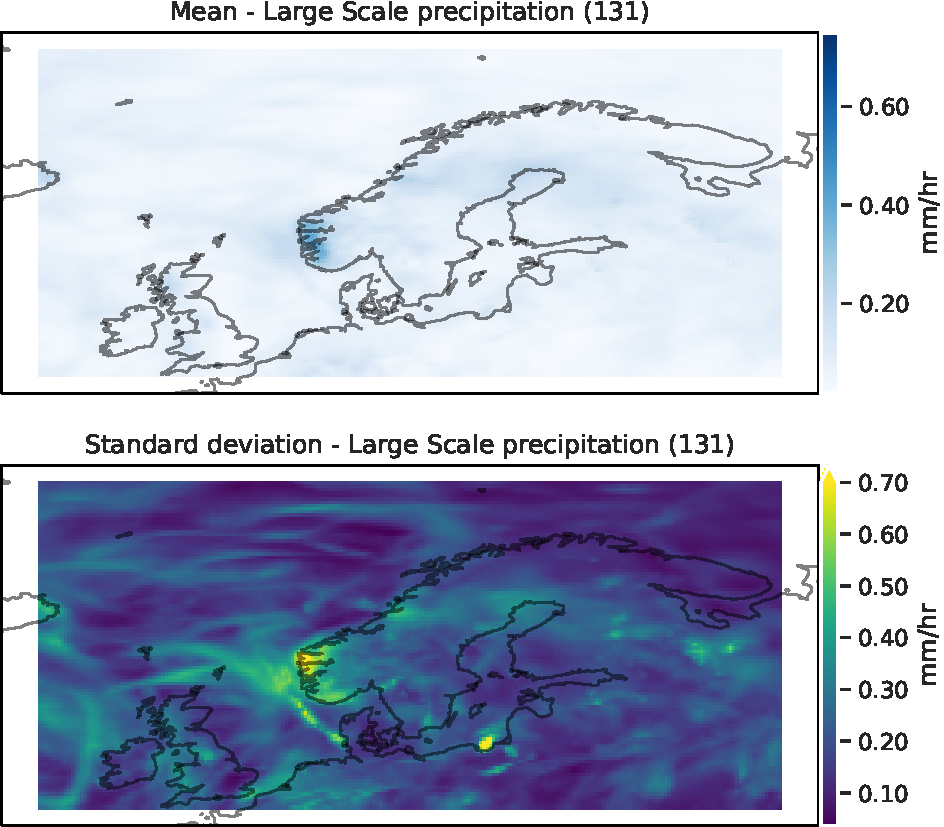
\includegraphics[width=\textwidth]{Figures/lsPVest.pdf}
    \caption{Large scale precipitation for cases in West zone.}
    \label{fig:WestlsP}
\end{subfigure}
\begin{subfigure}[b]{0.49\textwidth}
    \centering
    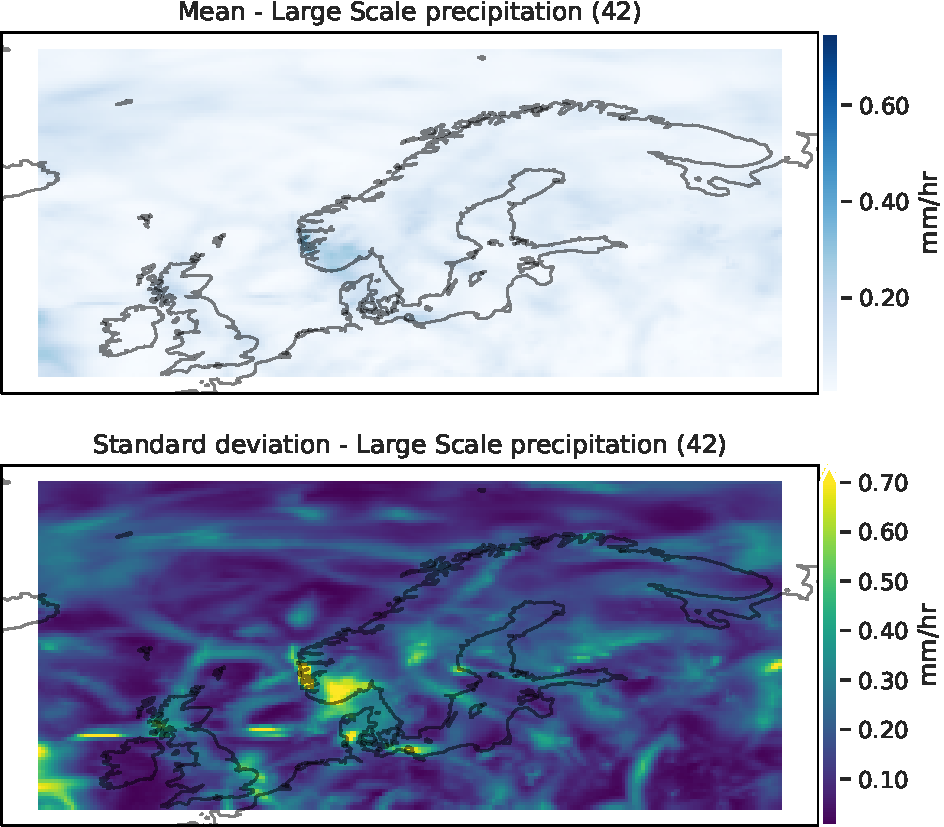
\includegraphics[width=\textwidth]{Figures/lsPSor.pdf}
    \caption{Large scale precipitation for cases in South zone.}
    \label{fig:SouthlsP}
\end{subfigure}
\caption{Large scale precipitation composites for both \acrshort{htl} and \acrshort{fwtl} cases in different geographical zones. Included are cases where height information was \textit{not} provided in the Avinor data set.}
\label{fig:largescalezones}
\end{figure}

\begin{figure}[H]
     \centering
     \begin{subfigure}[b]{0.49\textwidth}
         \centering
         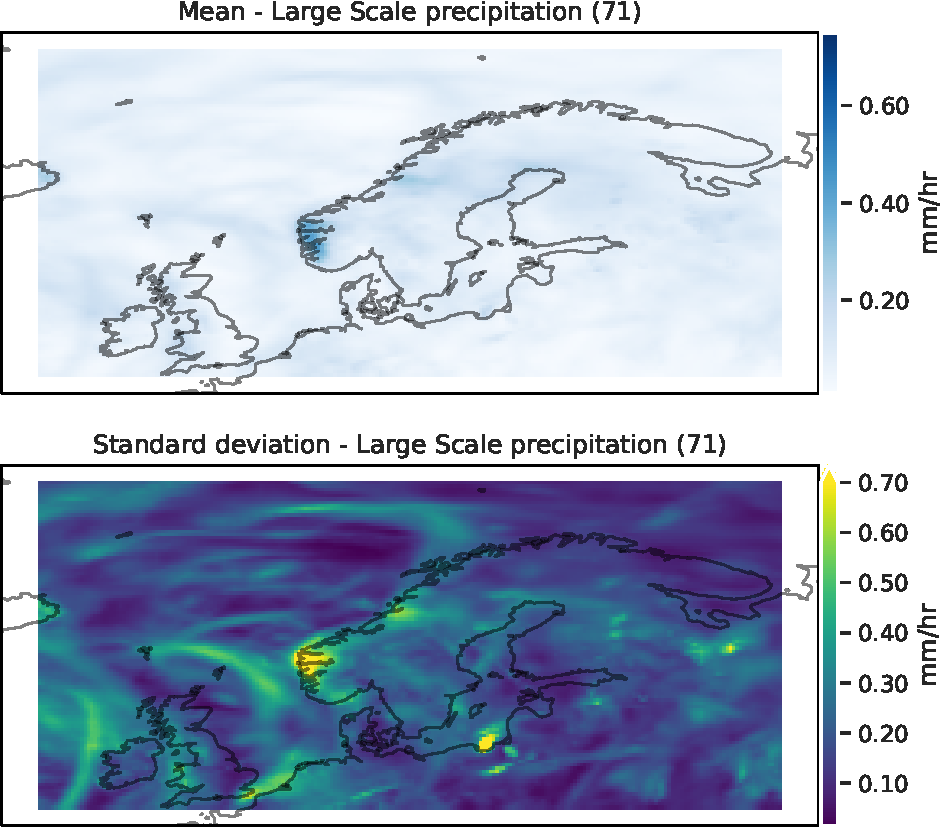
\includegraphics[width=\textwidth]{Figures/lsPENBR.pdf}
         \caption{Large scale precipitation for cases at  Flesland.}
         \label{fig:ENBRlsP}
     \end{subfigure}
     \hfill
     \begin{subfigure}[b]{0.49\textwidth}
         \centering
         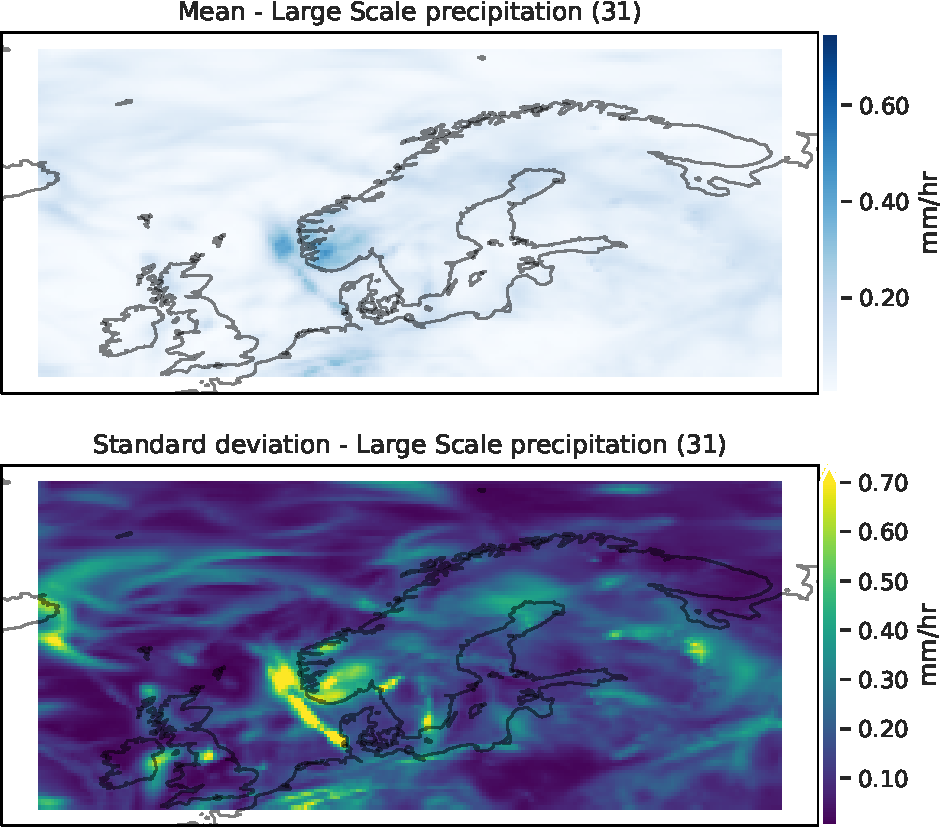
\includegraphics[width=\textwidth]{Figures/lsPENZV.pdf}
         \caption{Large scale precipitation for cases at Sola.}
         \label{fig:ENZVlsP}
     \end{subfigure}

    \begin{subfigure}[b]{0.5\textwidth}
    \centering
    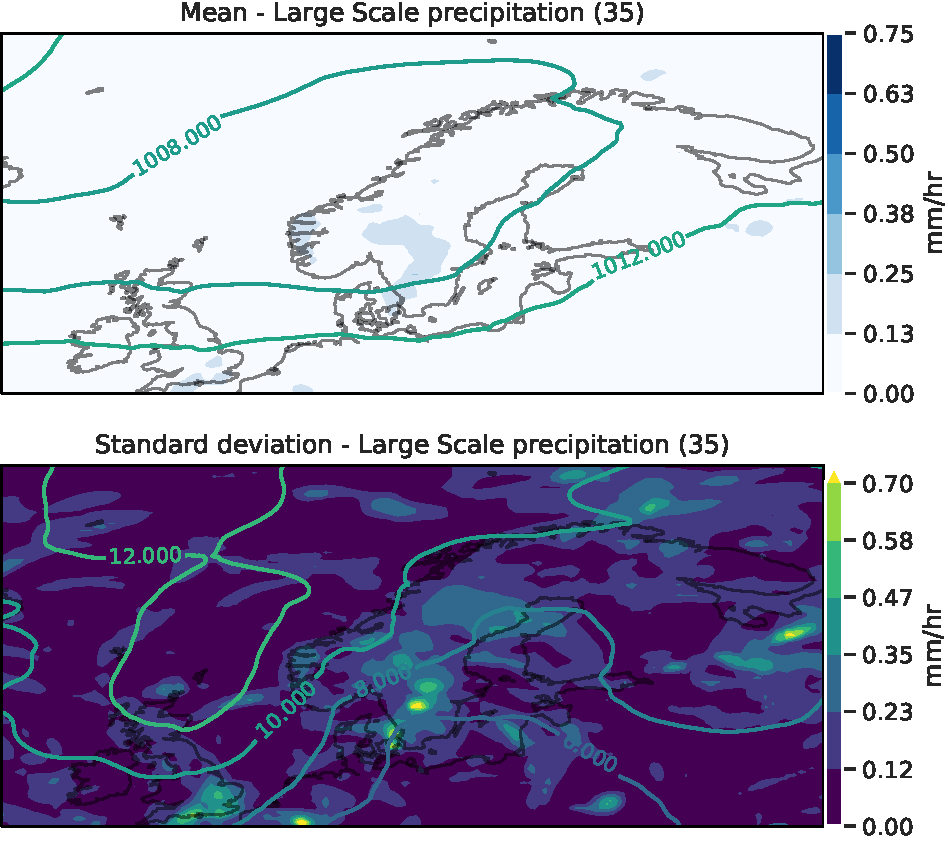
\includegraphics[width=\textwidth]{Figures/lsPENGM.pdf}
    \caption{Large scale precipitation for cases at Gardermoen.}
    \label{fig:ENGMlsP}
\end{subfigure}
\caption{Same as for Figure \ref{fig:largescalezones}, but for only the biggest airports}
\label{fig:largescaleairports}
\end{figure}

\subsubsection{Convective precipitation}
Now, considering the convective precipitation as shown in Figure \ref{fig:convectivezones}, there are clear convective systems precipitating in all zones, even in the South zone. The standard deviation is also somewhat high, but this is to be expected when considering the chaotic nature of convective precipitation. This standard deviation is also higher than the mean value in some cases, which also hints to a problem of placing convective scale systems, as was the case for the coastal zones discussed in Section \ref{sec:verticalvelocity}. The cases near the airports are shown in Figure \ref{fig:convectiveairports}. Flesland and Sola show the same picture as the previous figure in that there is a large precipitation intensity along the west coast, but high standard deviation, especially around Sola in the Sola case and around Flesland in the Flesland case. Here, Gardermoen also has very clearly convective precipitation related to the triggered lightning events. 

\begin{figure}[H]
\begin{subfigure}[b]{0.49\textwidth}
    \centering
    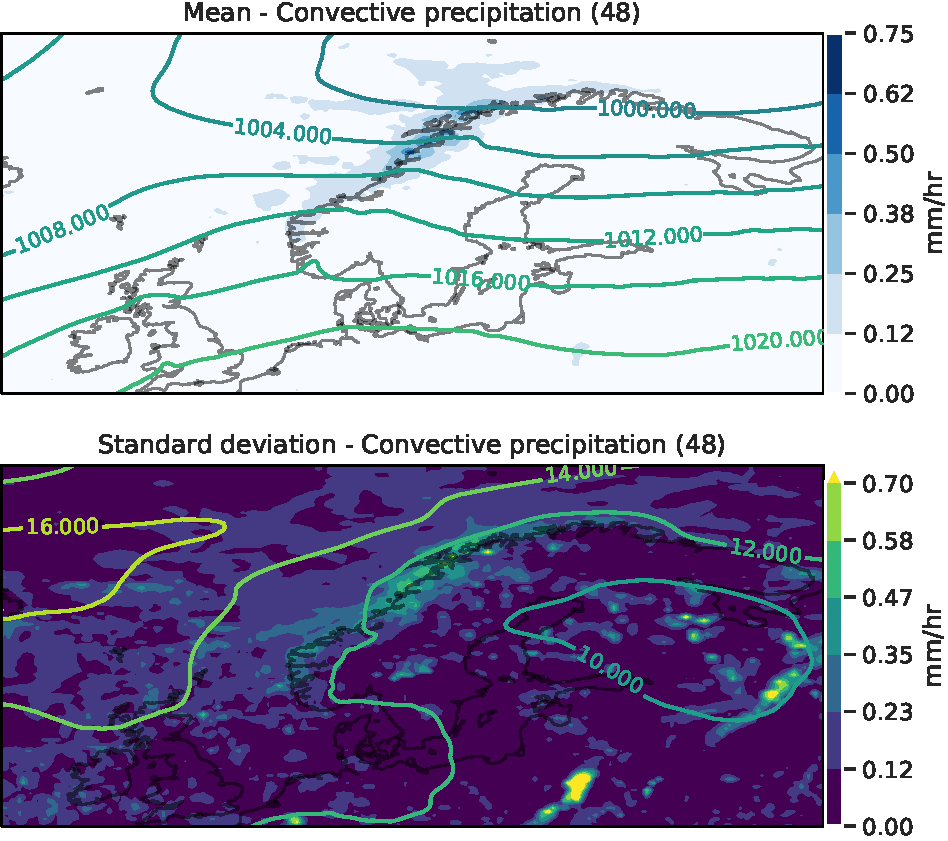
\includegraphics[width=\textwidth]{Figures/cPNord.pdf}
    \caption{Convective precipitation for cases in North zone.}
    \label{fig:NordcP}
\end{subfigure}
\begin{subfigure}[b]{0.49\textwidth}
    \centering
    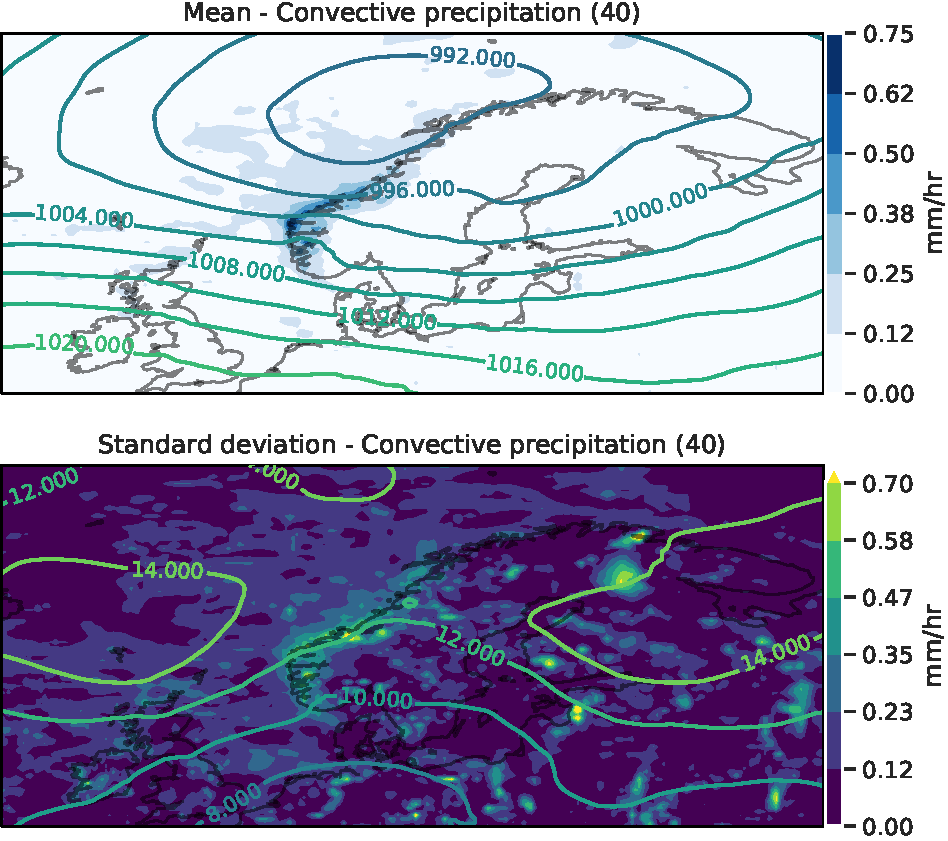
\includegraphics[width=\textwidth]{Figures/cPNordvest.pdf}
    \caption{Convective precipitation for cases in Northwest zone.}
    \label{fig:NordWestcP}
\end{subfigure}
\begin{subfigure}[b]{0.49\textwidth}
    \centering
    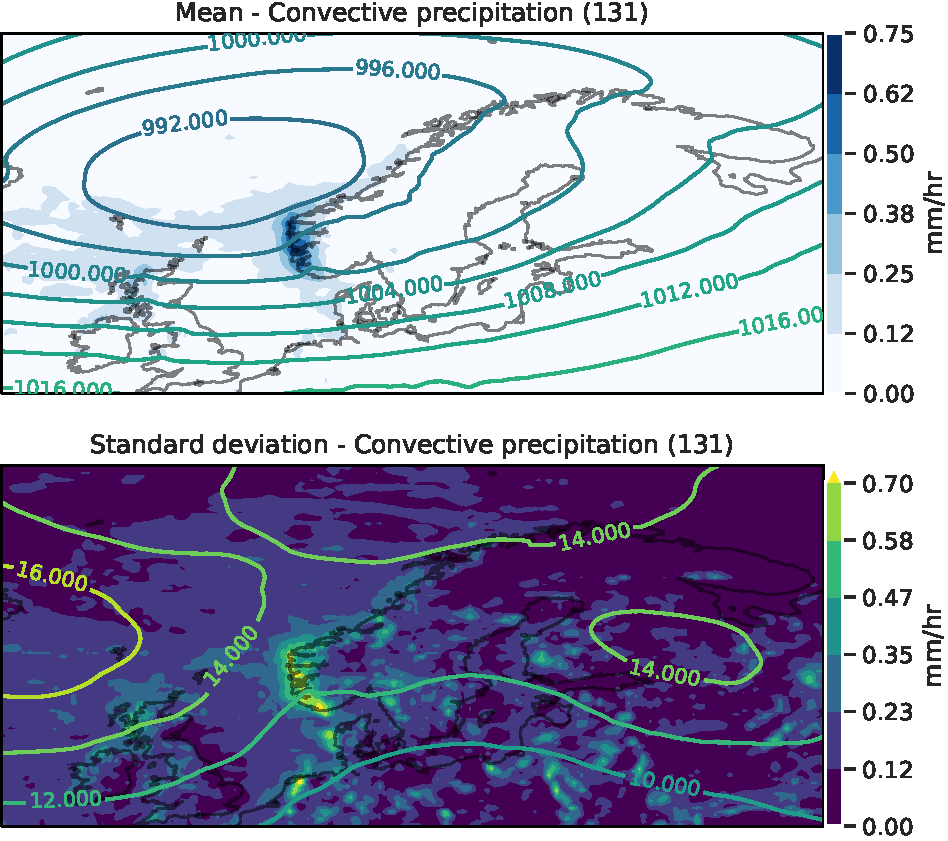
\includegraphics[width=\textwidth]{Figures/cPVest.pdf}
    \caption{Convective precipitation for cases in West zone.}
    \label{fig:WestcP}
\end{subfigure}
\begin{subfigure}[b]{0.49\textwidth}
    \centering
    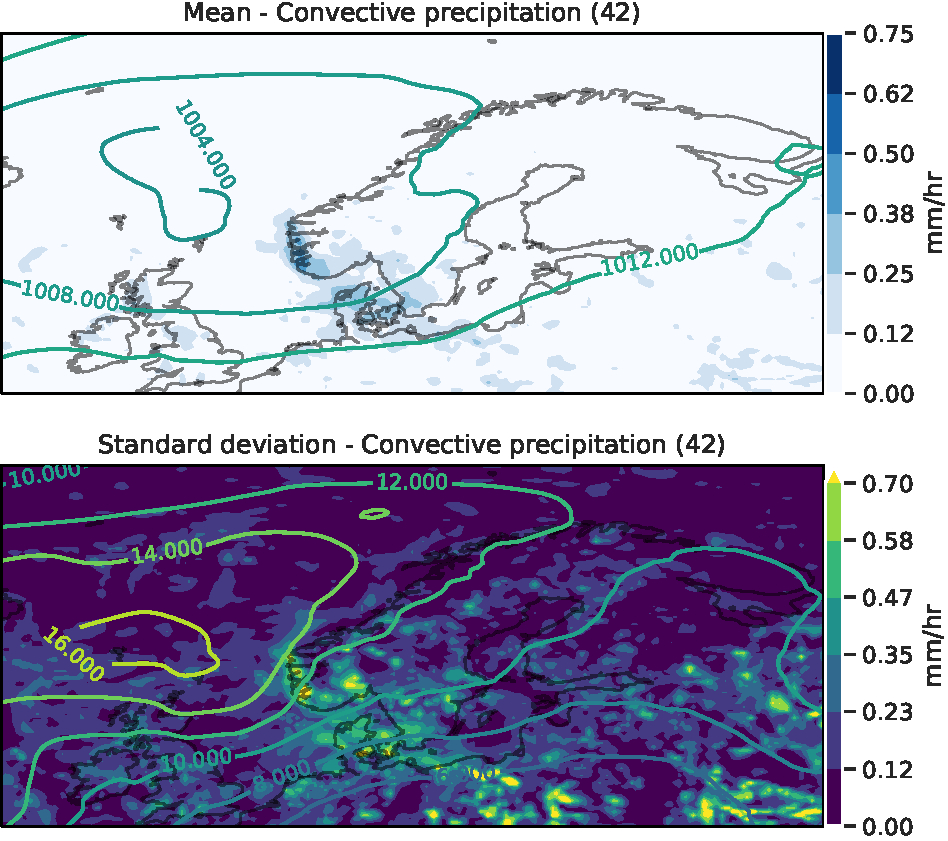
\includegraphics[width=\textwidth]{Figures/cPSor.pdf}
    \caption{Convective precipitation for cases in South zone.}
    \label{fig:SouthcP}
\end{subfigure}
\caption{Convective precipitation composites for the different zones}
\label{fig:convectivezones}
\end{figure}

\begin{figure}[H]
     \centering
     \begin{subfigure}[b]{0.49\textwidth}
         \centering
         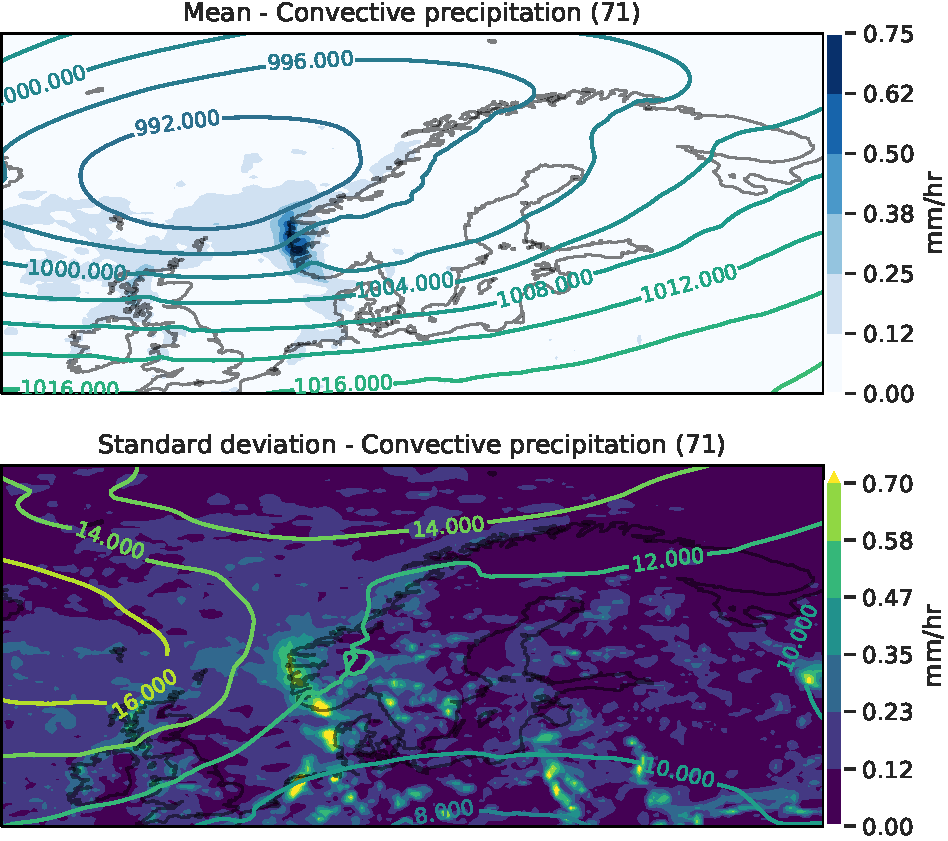
\includegraphics[width=\textwidth]{Figures/cPENBR.pdf}
         \caption{Convective precipitation for cases at Flesland}
         \label{fig:ENBRcP}
     \end{subfigure}
     \hfill
     \begin{subfigure}[b]{0.49\textwidth}
         \centering
         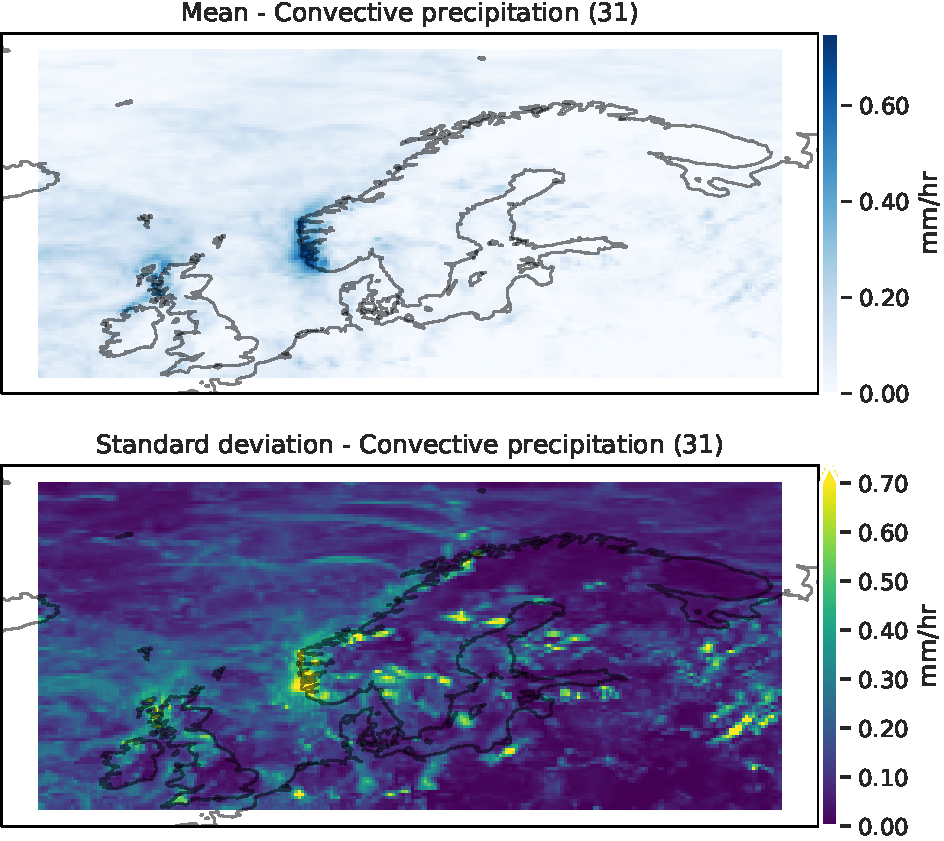
\includegraphics[width=\textwidth]{Figures/cPENZV.pdf}
         \caption{Convective precipitation for cases at Sola}
         \label{fig:ENZVcP}
     \end{subfigure}

    \begin{subfigure}[b]{0.5\textwidth}
    \centering
    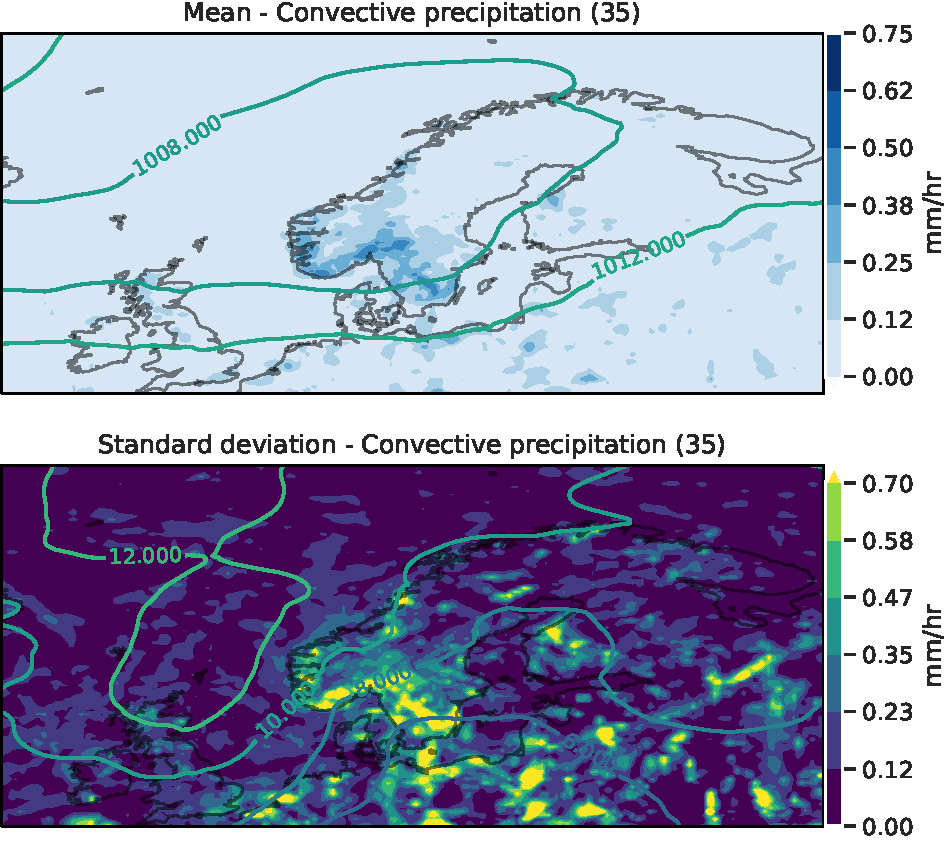
\includegraphics[width=\textwidth]{Figures/cPENGM.pdf}
    \caption{Convective precipitation for cases in Gardermoen zone.}
    \label{fig:ENGMcP}
\end{subfigure}
\caption{Convective precipitation composites for the biggest airports. }
\label{fig:convectiveairports}
\end{figure}

\subsection{Why are there more HTL near Flesland than near Sola?}

Looking at the flight traffic data compared to triggered lightning events in Table \ref{tab:traffic}, it is clear that Flesland airport has the highest incident per traffic ratio of the large Norwegian airports. 
Figure \ref{fig:metarclimat} shows Flesland to have a higher (20$\%$) frequency of rain than Sola at 15$\%$. The same is seen for both categories of showers (\textit{SH}, \textit{VCSH}). This suggests a more convective area around Flesland airport than at Sola airport. Ørlandet has similar convective activity to Flesland, but has almost no commercial air traffic. Therefore, any triggered lightning incident would not be in this data set and there is a smaller amount of potential trigger events. 

This convective difference between Flesland and Stavanger cannot be explained by yearly traffic differences, and their geographical positions are so close that there should not be any substantial climatological temperature differences between the two. There is somewhat less lightning activity observed at Flesland compared to Sola. As discussed in \ref{sec:pressure}, the local topography seems to be important for triggered lightning incidents. As such Flesland airport is situated among mountains, whilst Sola airport is in a flatter area.

\begin{table}[H]
        \begin{tabular}{r|l|l|l|}
            & Sola (ENZV) & Flesland (ENBR) & Gardermoen (ENGM) \\\hline
            Average yearly traffic (2016-2018)  & 74 532 & 92 128 & 253 599   \\\hline
            Lightning close to airport (2008-2019) & 30 920 & 22 774 & 68 321 \\\hline
            Cases close to airport & 24 & 63  & 35 \\\hline
            Case per traffic  & 1 / 31 055 & 1 / 14 624 & 1 / 72 457 \\\hline
            Case per recorded lightning & 1 / 1 289 & 1 / 361 & 1 / 1 952 \\\hline
        \end{tabular}
     \caption{Average traffic, accumulated lightning activity, and cases within $0.5^{\circ}$($\approx 50km$) radius of the three biggest Norwegian airports.}
     \label{tab:traffic}
\end{table}


\section{Implications of precipitation error in HTI}
As stated in Section \ref{sec:precipbug}, an error has been found in the usage of precipitation data when forecasting \acrshort{hti}. The error was usage of \textit{accumulated} precipitation instead of \textit{hourly} precipitation in the forecast. A complete case-by-case effect of this is shown in the figures in Appendix \ref{app:A}. Figure \ref{fig:fixeffect} shows the effect of considering hourly instead of accumulated precipitation\footnote{Maps showing the effect for the whole domain are moved to Appendix \ref{app:A}}. Shown is an approximate halving of the frequency of Yellow risk for all airports. The higher risk categories (Orange and Red) are only substantially reduced at northfacing airports, i.e. airports in the northwest and North zone. Sola and Flesland see a halving in the Orange category, but not a substantial reduction in the Red. Flesland and Sola have approximately the same frequency of Red and Orange forecasts, but as shown in \ref{tab:traffic}, Flesland has double the amount of \acrshort{htl} and \acrshort{fwtl} cases.

To further investigate whether this leads to any reduction in \acrshort{hti} forecast skill, \acrshort{metar} data was considered to verify that \acrshort{hti} correctly identifies coastal and off-shore convective activity. Thus, the effect for the three airports from the North zone are shown in Figure \ref{fig:HTIMETAR1}. The figure shows a clear increase in frequency of non-White risk categories for all three airports. Hammerfest and Bodø have a slight increase in \acrshort{htl}-related phenomena forecasted as White (Here, snow and showers.) However, there is also some reduction in other phenomena such that this seems to be a non-substantial increase. The same is observed for Figure \ref{fig:HTIMETAR2}, which shows the risk categories for the three northwestern coastal airports: a clear increase in frequency of non-White risk categories when convective activity is observed. It should be noted that there seems to be no clear total increase or decrease in the White category for all three airports. In all, the skill of the \acrshort{hti} does not seem to be reduced, but rather increased by taking into account the hourly precipitation. %The argument for a reduction can be made, due to a known bug in the HARMONIE-configuration used at MEPS, leading to an underrepresentation of precipitation along the coast of Norway. \cite{Morten_private}

\begin{figure}[H]
    \centering
     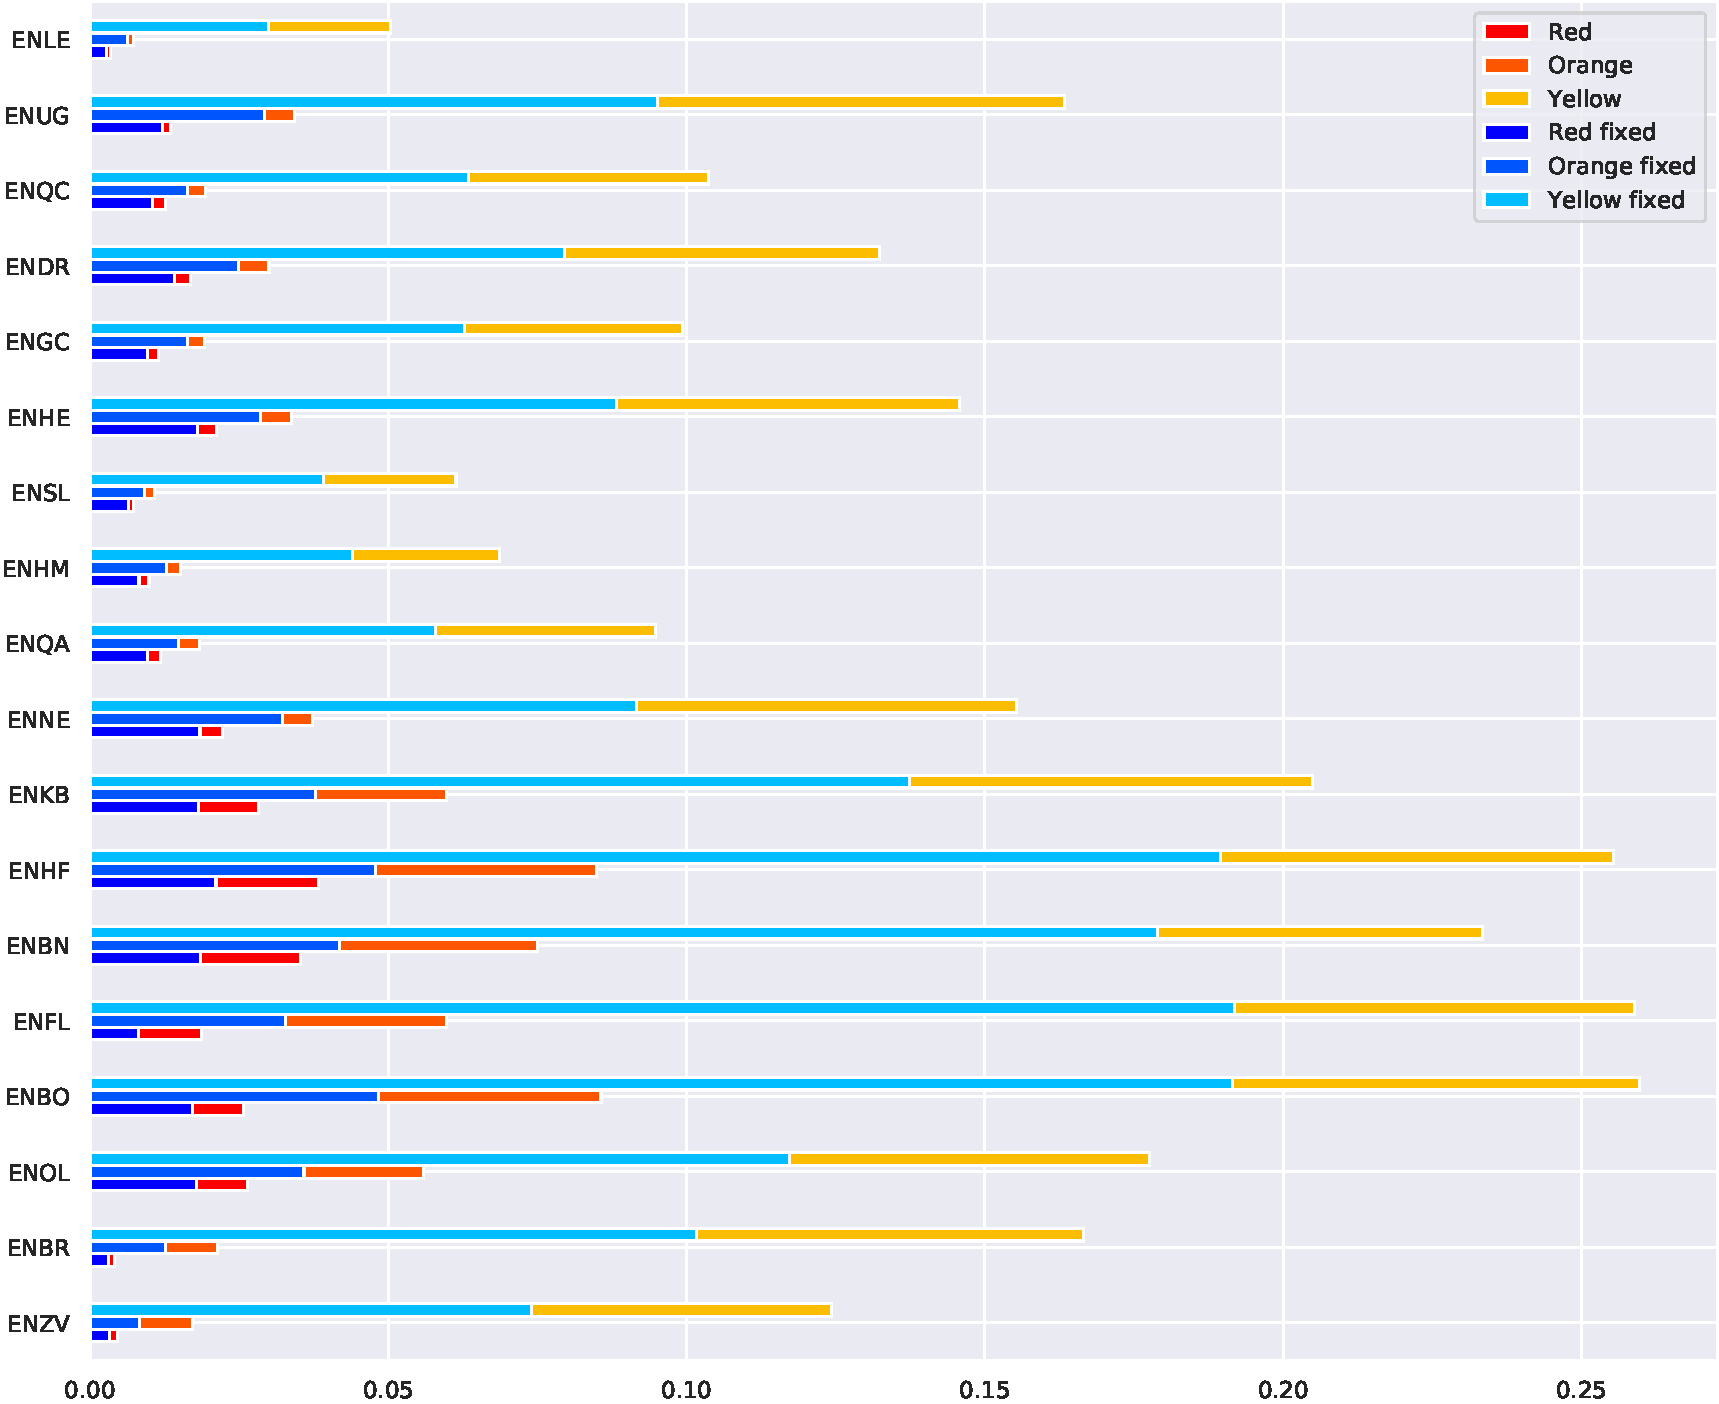
\includegraphics[width=\textwidth]{Figures/fixeffect.pdf}
    \caption{Frequency of \acrshort{hti}-risk levels during \acrshort{htl}-season (October-April), before and after fixing the erroneous forecast, for selected airports.}
    \label{fig:fixeffect}
\end{figure}

\begin{figure}[H]
    \centering
    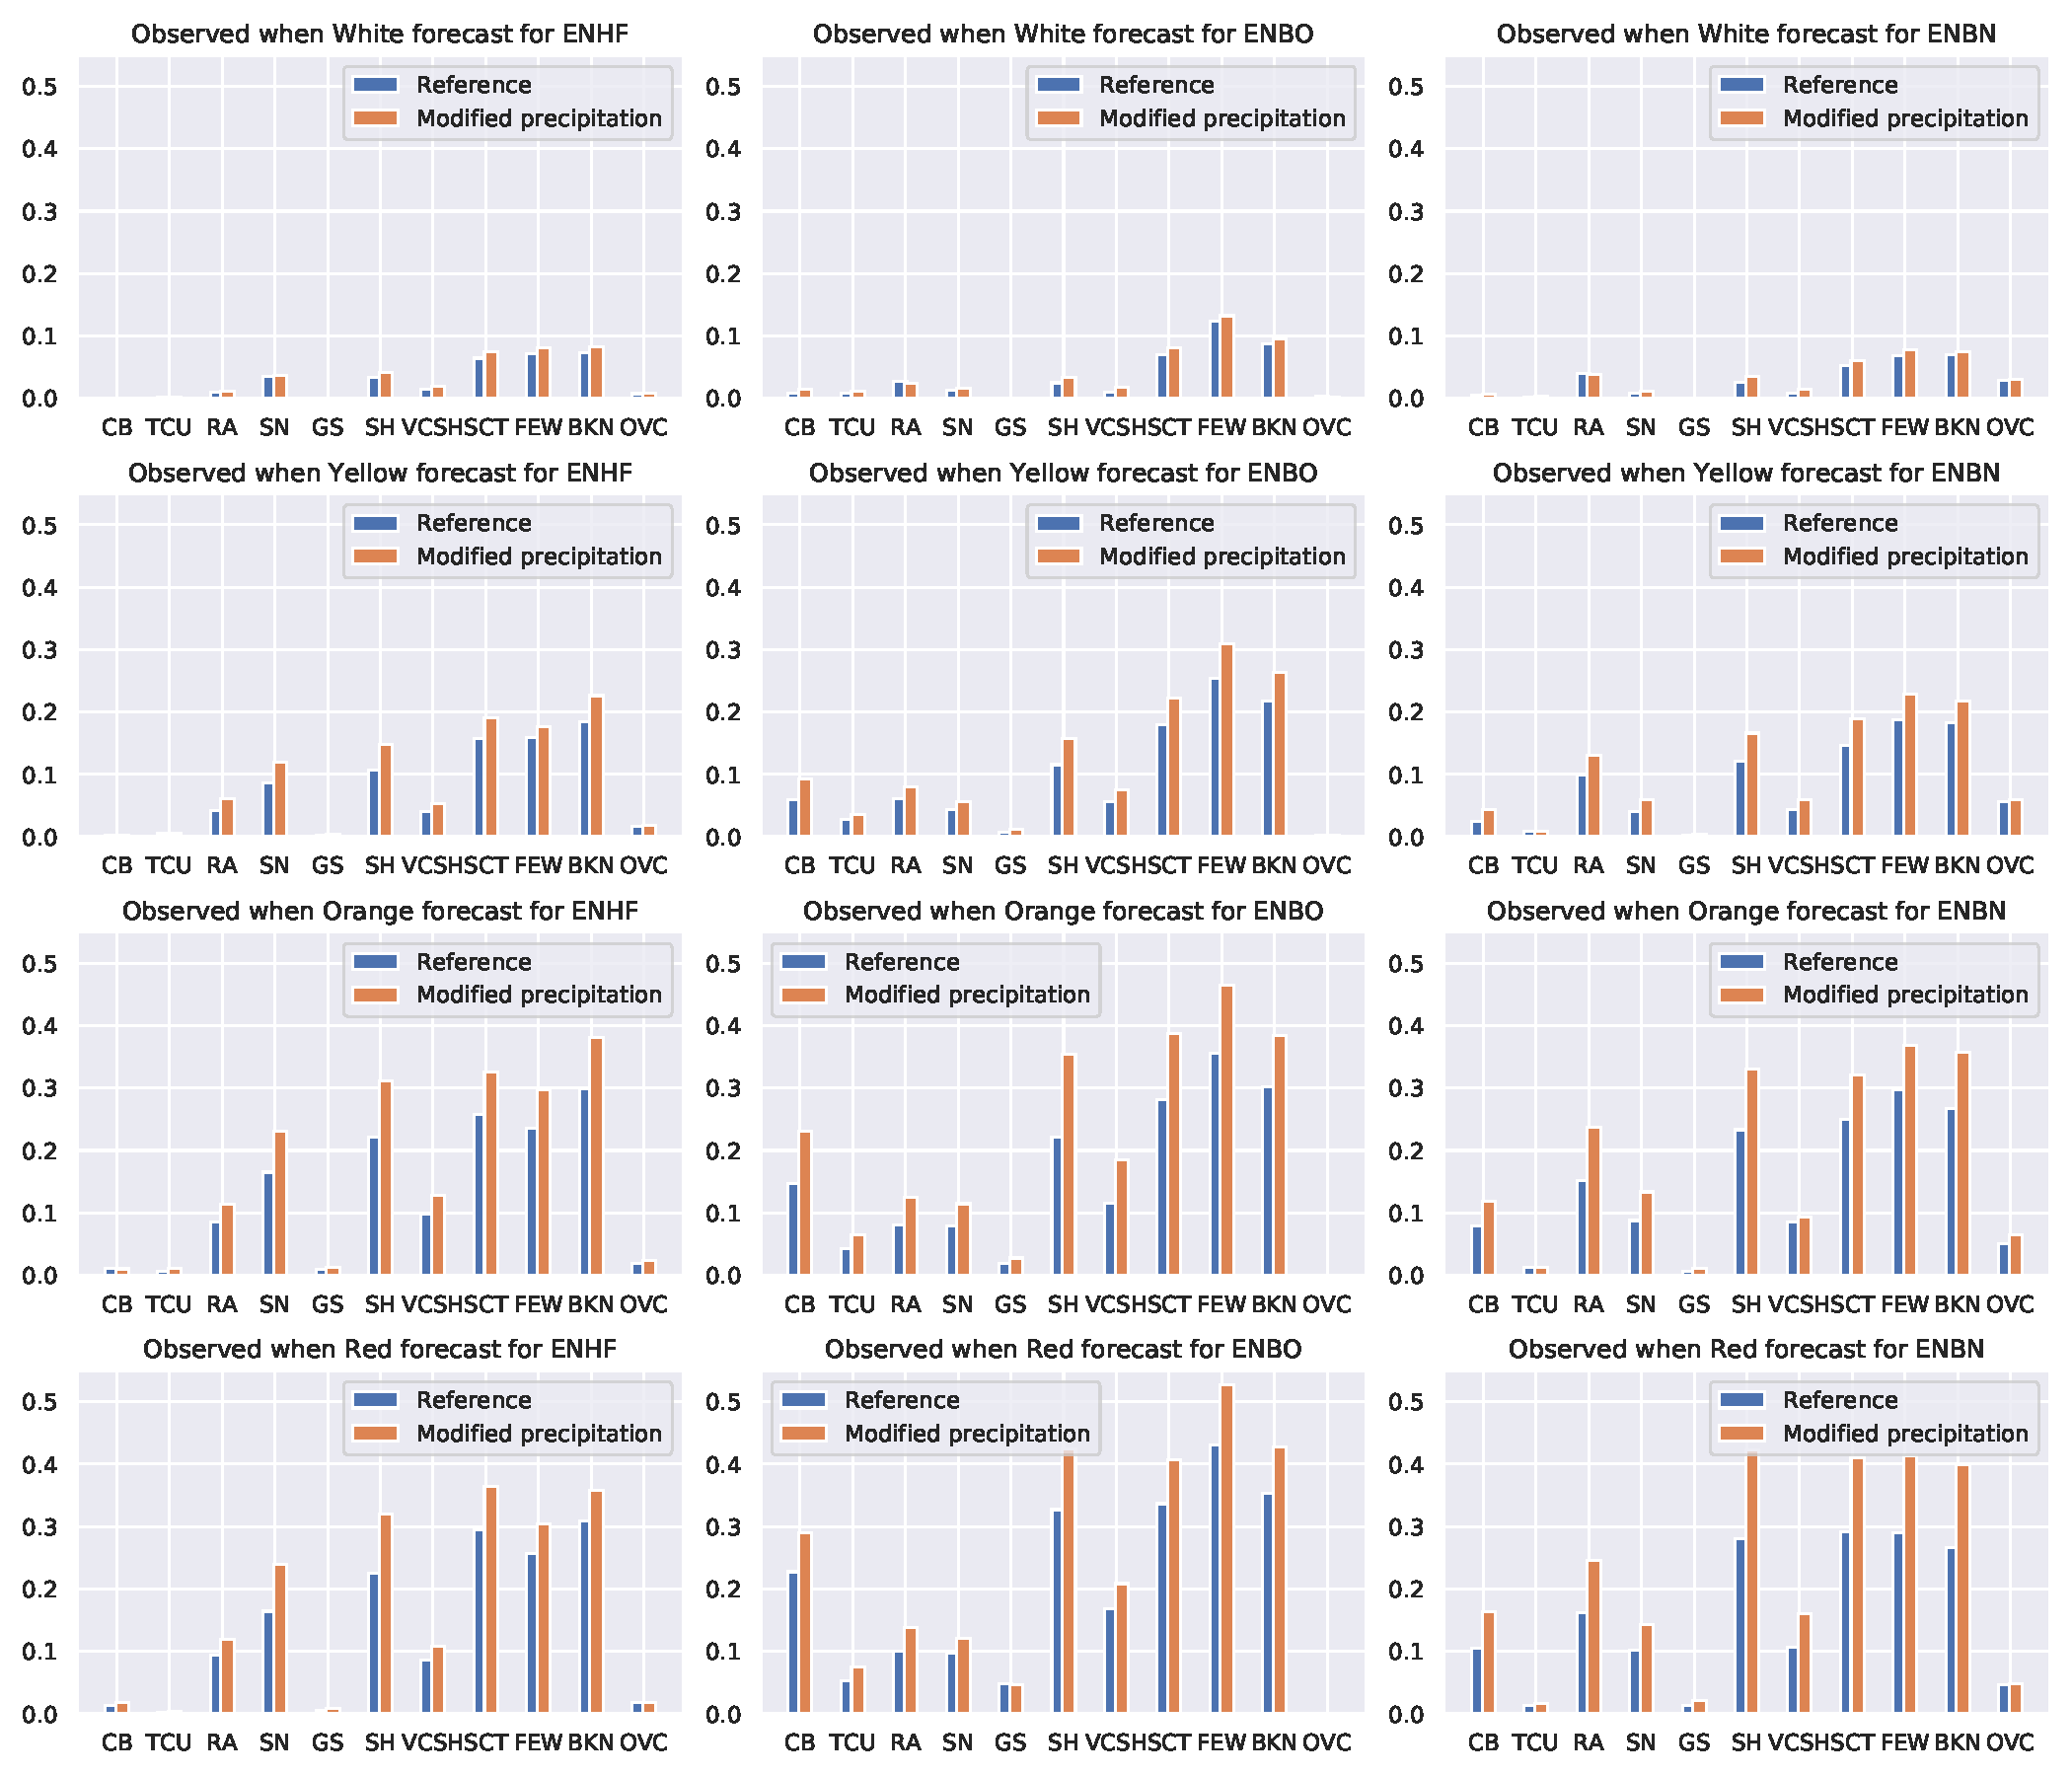
\includegraphics[width=\textwidth]{Figures/HTIMetar1.pdf}
    \caption{Frequency of \acrshort{hti}-risk given observed meteorological-phenomenon during \acrshort{htl}-season (October-April), for the three northernmost coastal airports: Hammerfest (ENHF), Bodø (ENBO), and Brønnøysund (ENBN)}
    \label{fig:HTIMETAR1}
\end{figure}

\begin{figure}[H]
    \centering
    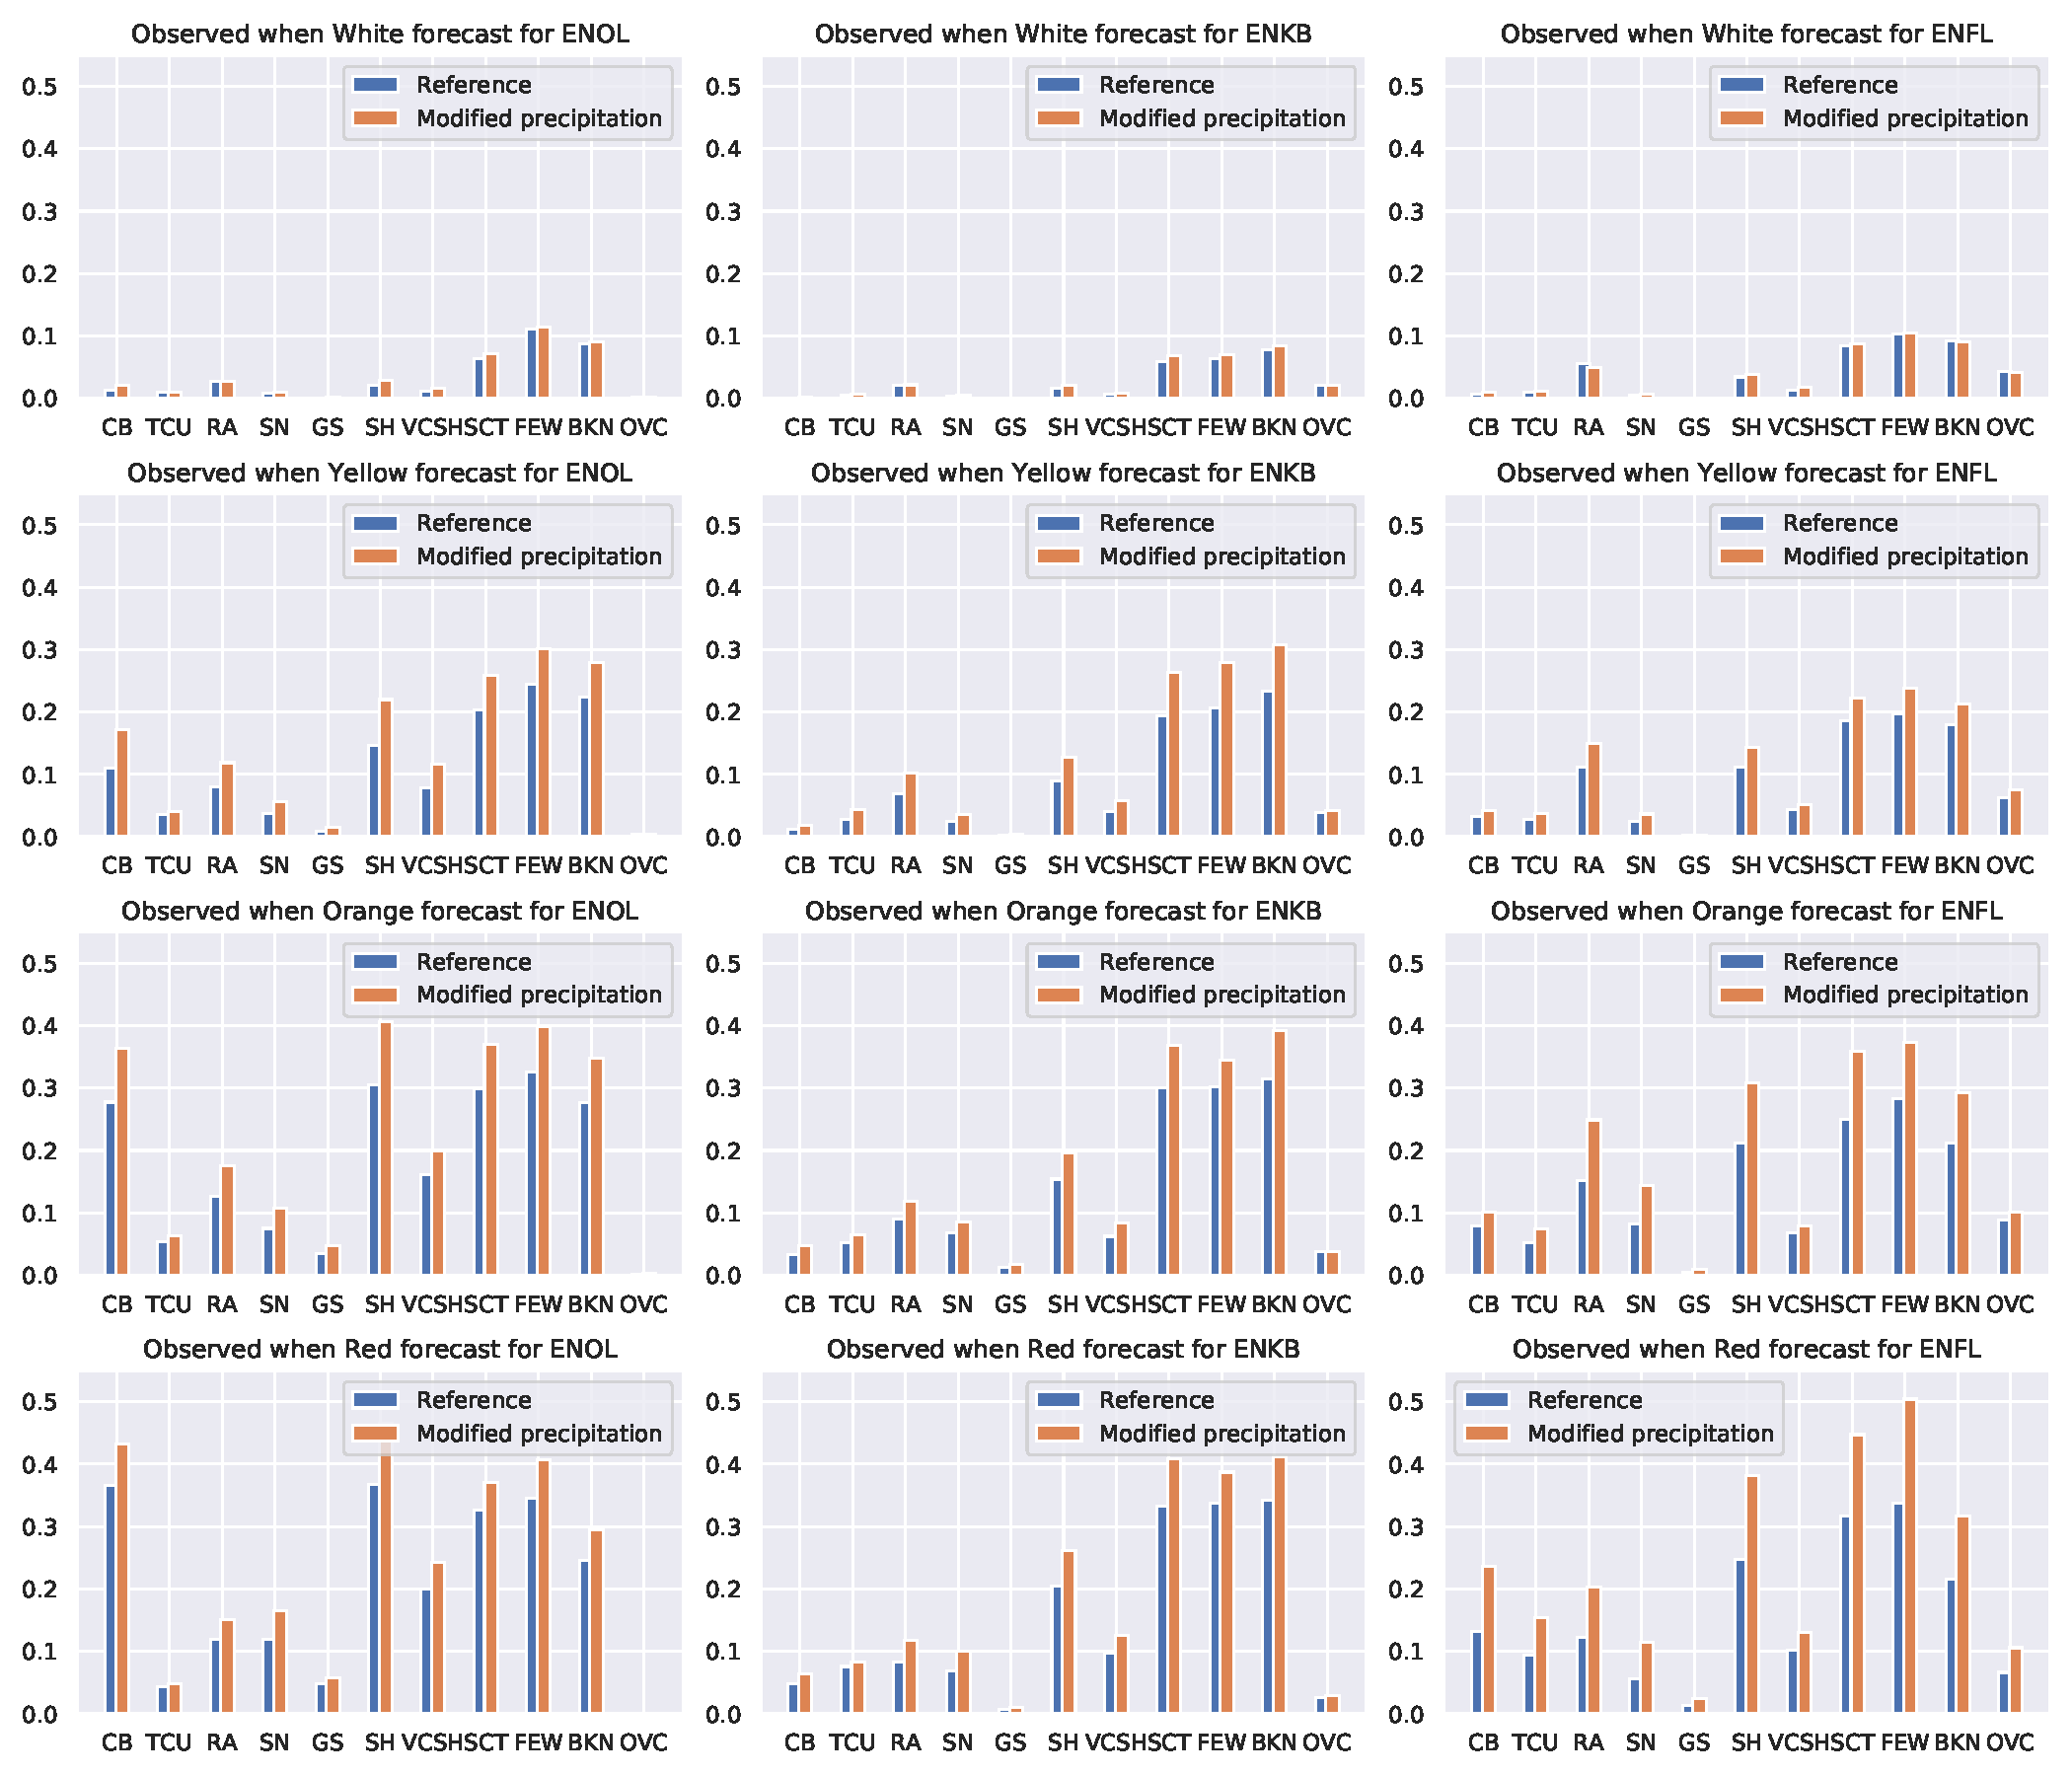
\includegraphics[width=\textwidth]{Figures/HTIMetar2.pdf}
    \caption{Frequency of \acrshort{hti}-risk given observed meteorological-phenomenon during \acrshort{htl}-season (October-April), for the three northwestern coastal airports: Ørlandet (ENOL), Kristiansund (ENKB), and Florø (ENFL)}
    \label{fig:HTIMETAR2}
\end{figure}


\section{Decompositional analysis of triggered lightning incidents}
As discussed in Section \ref{sec:decomposition}, calculating sub-indices of forecasted \acrshort{hti} during recorded incidents allows for investigation into which, if any, of the sub-indices was under-evaluating the \acrshort{hti} risk. As stated in Section \ref{sec:hti}, \acrshort{hti} is calculated to be representative for the $750m$ ($\approx 2500$ feet) altitude. Thus, the following discussion only pertains to what is forecast at this altitude, and not (necessarily) at the height of the incident, as was done in Section \ref{sec:compositesera5}.

Figure \ref{fig:HeliAccum} shows 11 \acrshort{htl} cases from the Avinor data set with the sub-indices stacked on top of each other. On the x-axis is the altitude (in feet) at which the helicopter was flying. The figure shows the \acrshort{hti} to be at least $0.5$ for all 11 cases, but no cases were forecasted as Red and only two cases were forecasted as Orange. This is summarized in Table \ref{tab:HeliCont}. Figure \ref{fig:HeliDecomp} shows the sub-indices clearly delineated so that one can see which of the indices are lacking. The temperature sub-index is full for all but the third case, which, when calculated, had a temperature of -.67 $^{\circ}C$. Increasing the temperature to full would not increase the risk level in this case. Further, it can also be seen that in two of the 11 cases, precipitation would have been reduced to almost 0 if hourly instead of accumulated precipitation was considered, thus reducing the risk level to White. The third case where precipitation would be almost 0, was already White, so a reduction in risk level would not be seen. The most variability is found in the cloud and vertical velocity parameters. It should be noted that vertical velocity has had a positive value for all the cases, meaning that the upper threshold of the vertical velocity sub-index may be too strict. The cloud parameter reduces the risk level substantially (from Red to Yellow) for four of the cases. 

Looking now at the Fixed wing cases in \ref{fig:FWAccum}, which shows the total \acrshort{hti} decomposed to the sub-indices, with the altitude of the aircraft in feet on the x-axis. It can be seen that ten of the 34 cases would have a reduction in \acrshort{hti} due to consideration of the hourly (and not accumulated) precipitation. Only for three cases would this give a decrease in risk level. Even though some of these fixed wing incidents are happening at higher altitudes (e.g. 7000 feet), we see a relatively high sub-index for some of them, suggesting that there may be some convective activity in the whole column. This is also summarized in Table \ref{tab:FWCont}. Looking at Figure \ref{fig:FWDecomp}, one can see that vertical velocity is non-zero for \textit{all} cases, showing the vertical velocity to be positive in the case of triggered lightning events - even though many cases might be situated above or below the $750m$ altitude. The precipitation sub-index is generally not affected by differing heights, since it is a measure of how much precipitation would reach the ground - not precipitation in each level. The temperature sub-index shows a somewhat bad relation to the \acrshort{fwtl}. 19 of the cases had zero contribution from the temperature. This could be solely due to the aircraft being situated above or below the $750m$ altitude, but still close to the 0 $^{\circ}C$ isotherm.

It is to be noted from Tables \ref{tab:HeliCont} and \ref{tab:FWCont} that even though four fixed wing cases were correctly identified as Red, 41$\%$ were below the Yellow threshold. For the helicopter cases, zero were correctly identified as Red, but only two of the 11 (18.2$\%$) were below the Yellow threshold. Further, the helicopter data set is heavily influenced by the fact that they were recorded after the operational forecasting started: Any Red events were warned against and helicopter pilots have had an increased participation and reporting during this period. This may have lead to a skewing of the data set towards the tail of the majority of the cases, as seen in Figure \ref{fig:temperatureera5}, where the helicopter cases do not have a peak at the expected 0$^{\circ}C$ isotherm.

\begin{figure}[H]
    \centering
    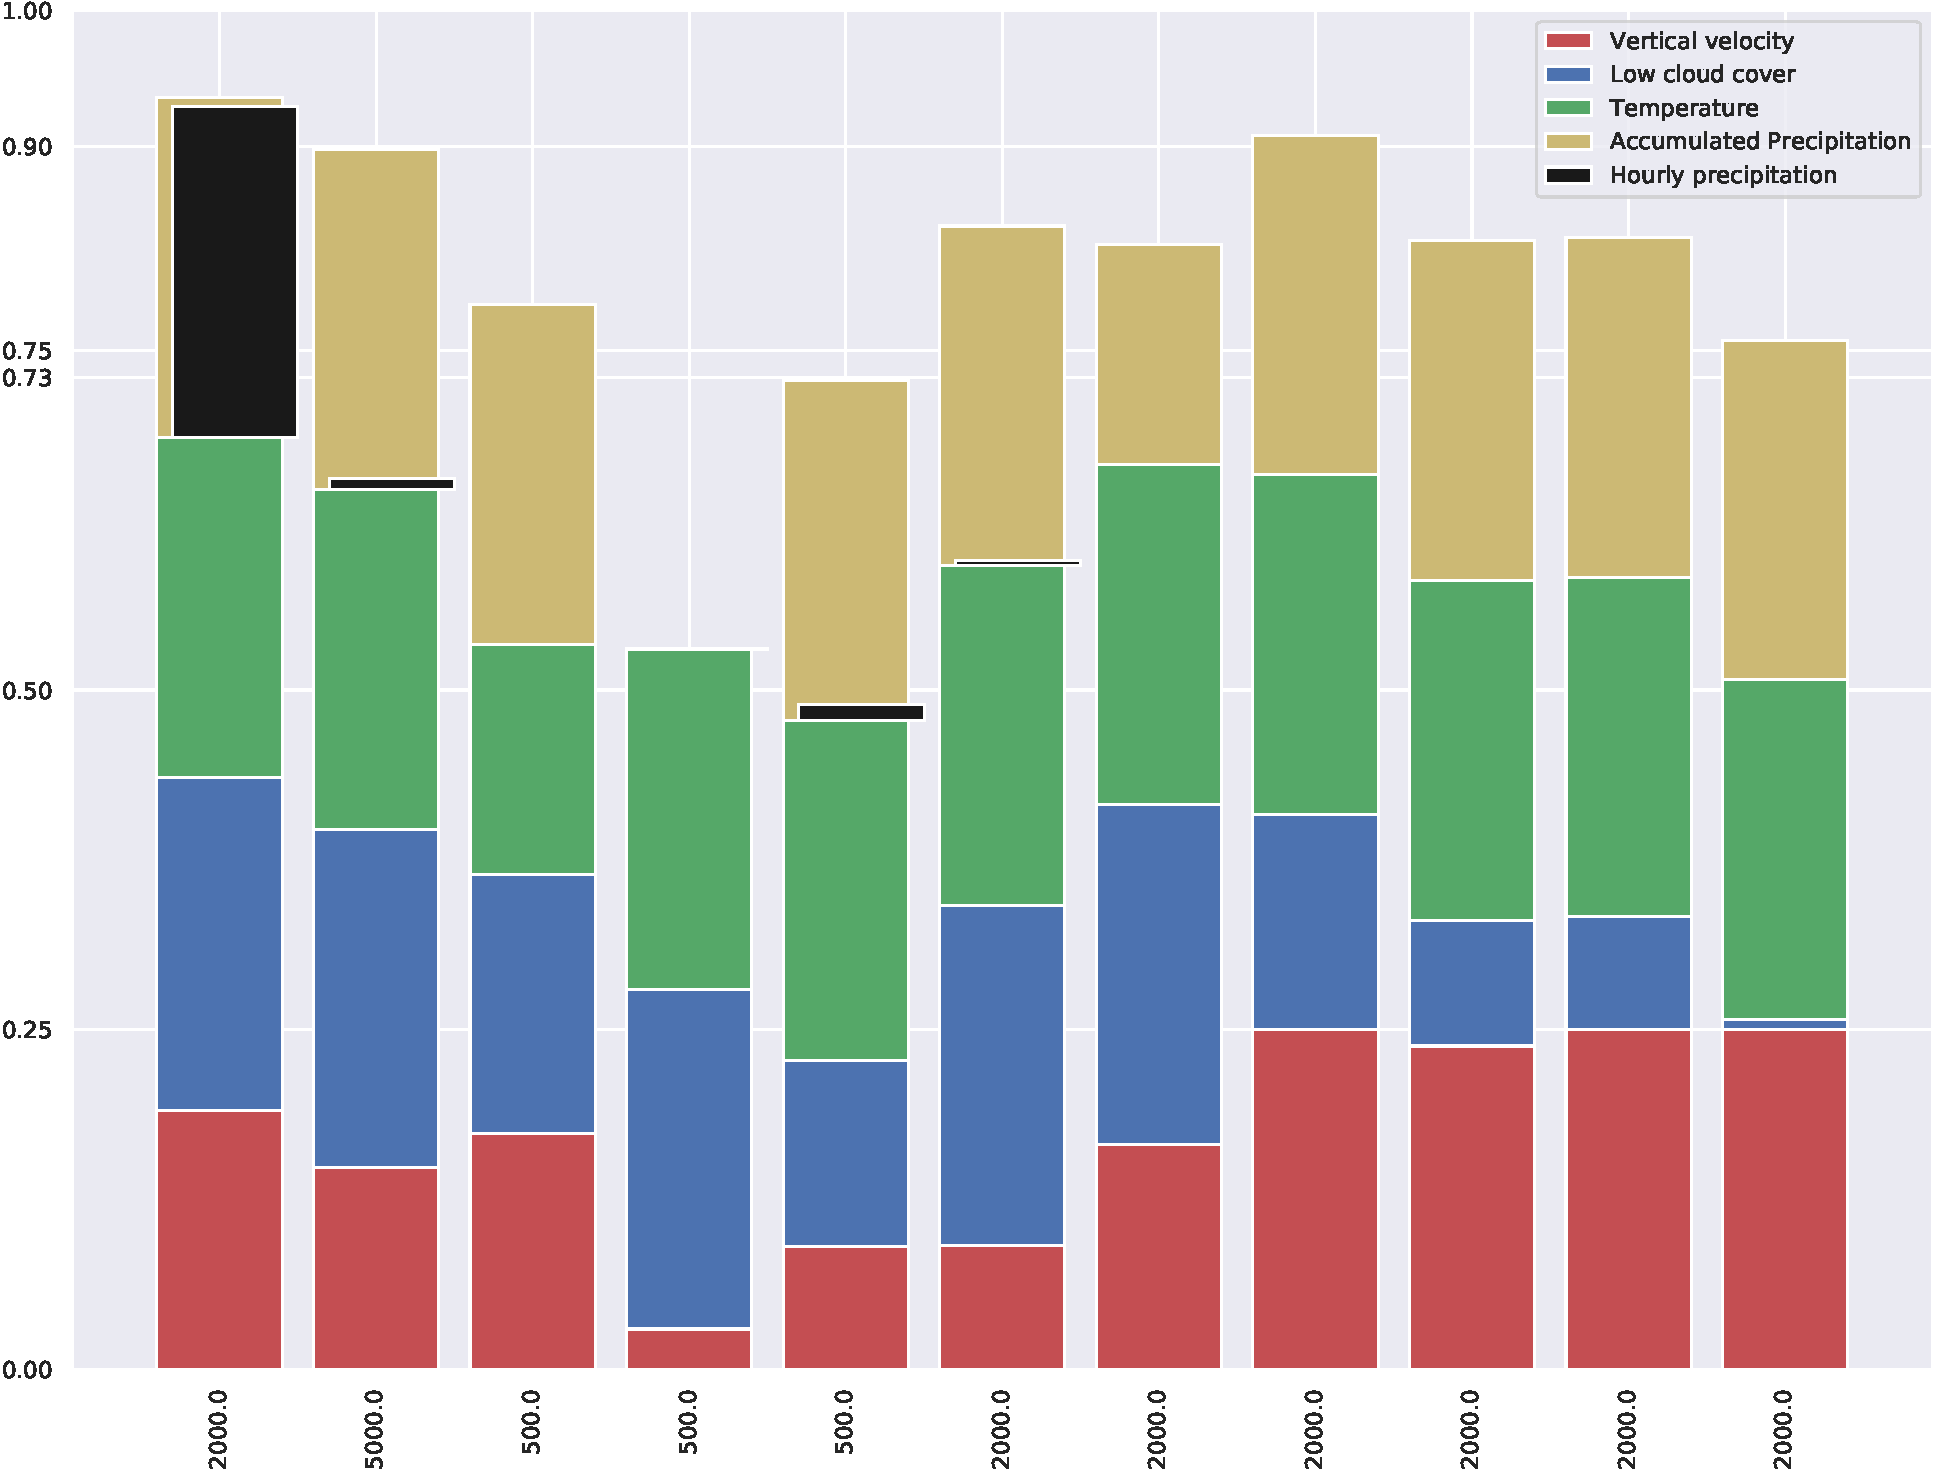
\includegraphics[width=\textwidth]{Figures/HeliAccum.pdf}
    \caption{Contributions from the different sub-indices, for Helicopter cases during the operational forecast. X-axis is height of incident in feet. Black on yellow is correction made by using the hourly precipitation instead of accumulated precipitation. Included are only cases from Avinor data set where position and height was available, for cases after November 2016.}
    \label{fig:HeliAccum}
\end{figure}

\begin{table}[H]
    \centering
    \begin{tabular}{c|c|c|c}
        Forecast & With Accumulated & Without Accumulated & Missed (\%) \\ \hline
        >Yellow (0.73) & 9 & 7 & 2 (18.2\%)\\
        >Orange (0.90) & 2 & 2 & 7 (63.6\%)\\ 
        >Red (0.99) & 0 & 0 & 11 (100\%)\\
    \end{tabular}
    \caption{Amount of cases forecast in each risk category based on the $11$ Helicopter cases in Figure \ref{fig:HeliAccum}. A Red risk is counted in Orange, and Yellow.}
    \label{tab:HeliCont}
\end{table}

\begin{figure}[H]
    \centering
    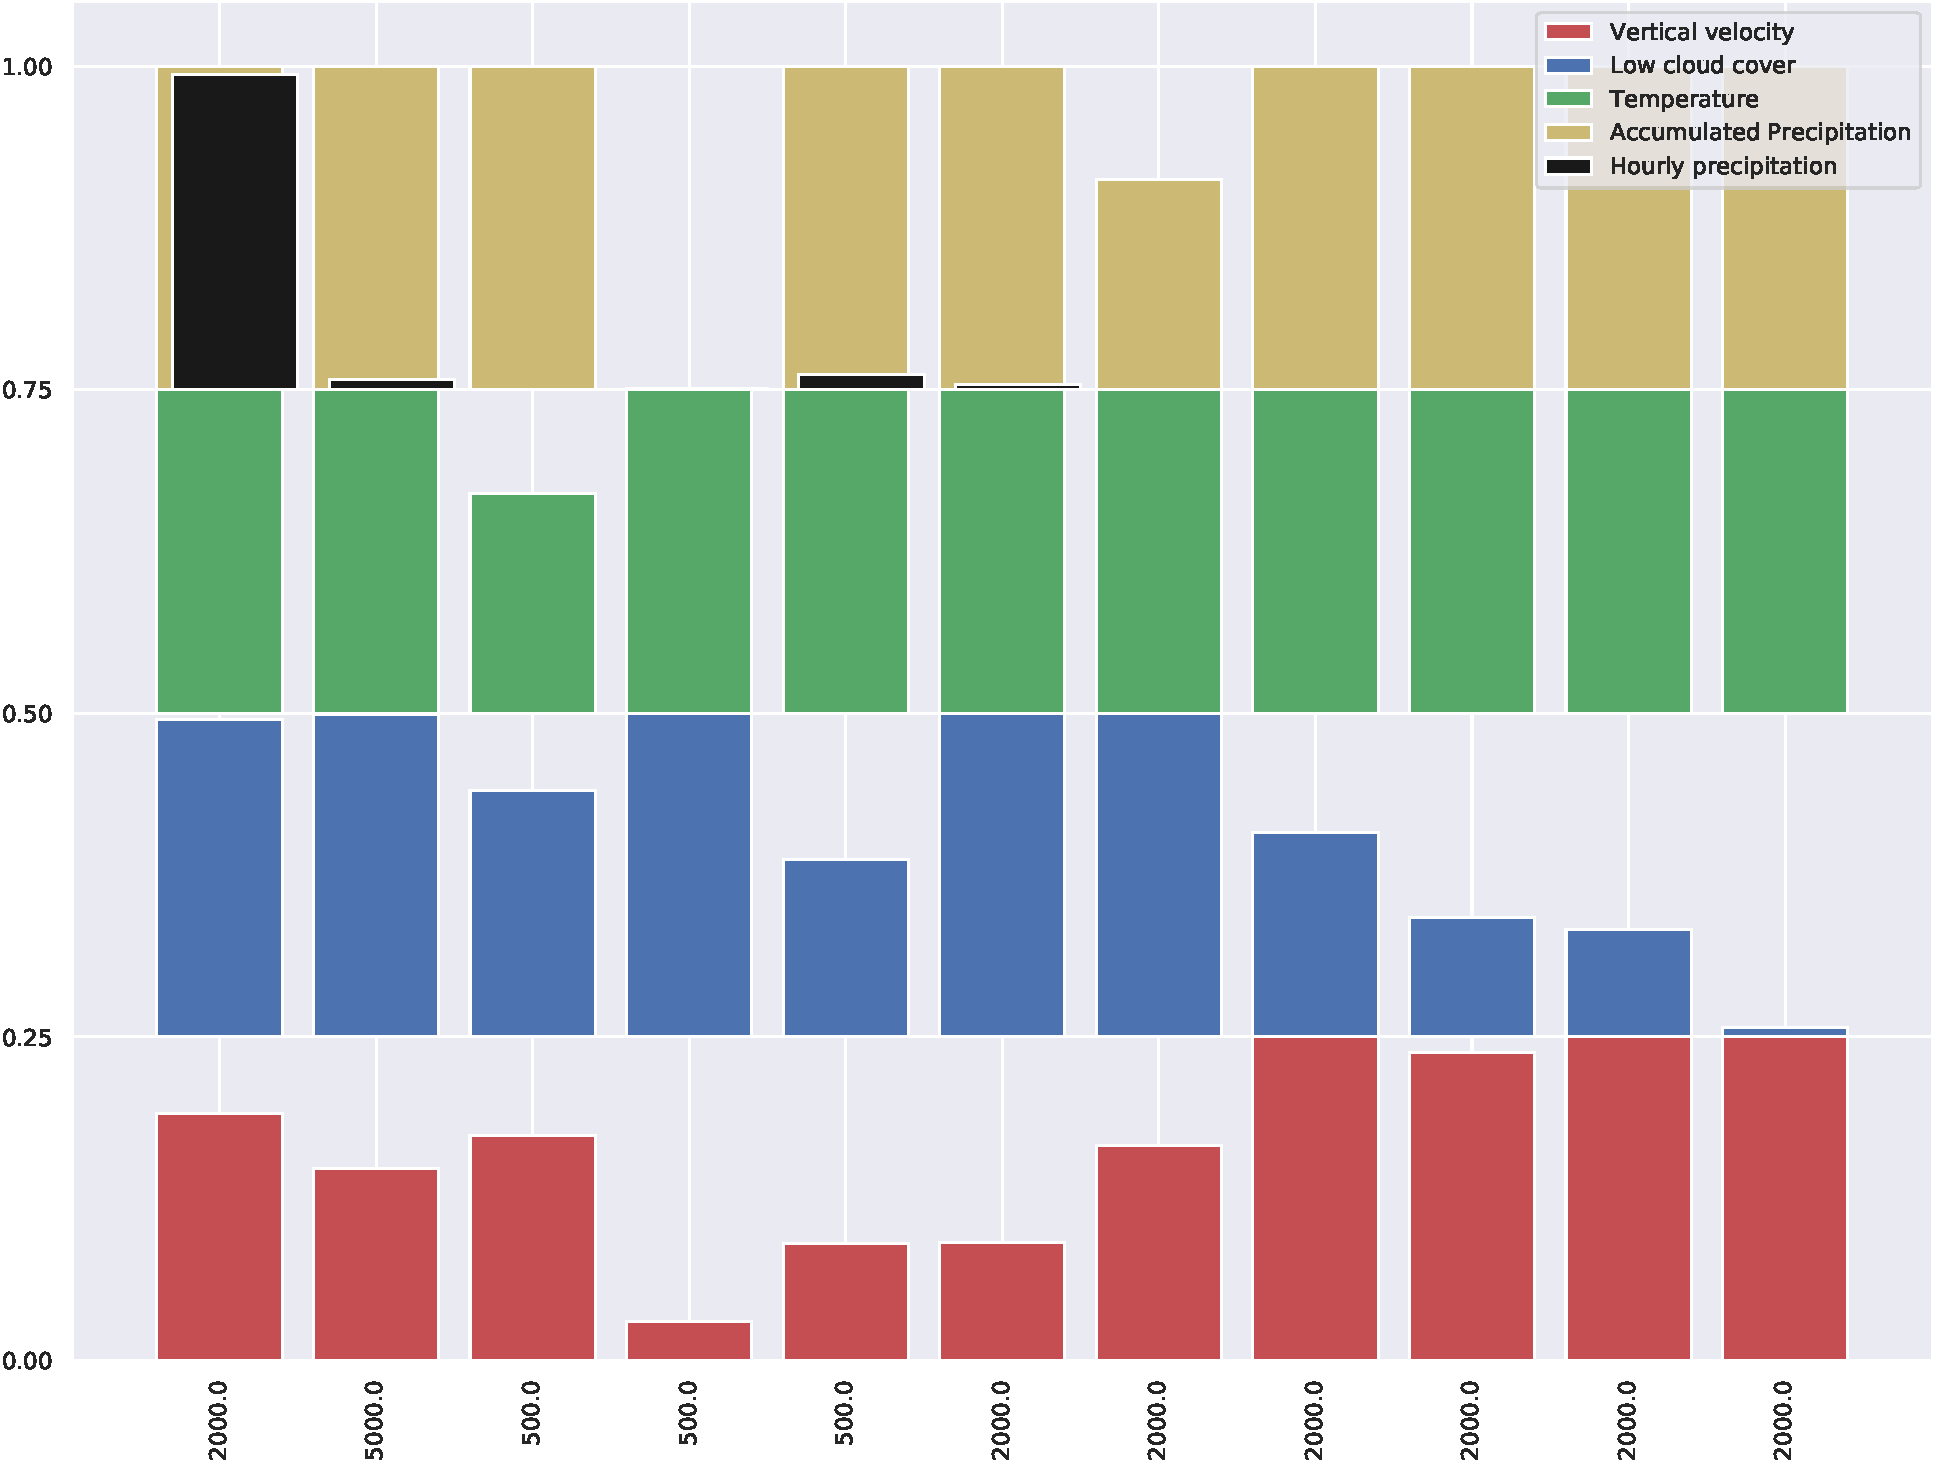
\includegraphics[width=\textwidth]{Figures/HeliDecomp.pdf}
    \caption{Same as \ref{fig:HeliAccum}, but clearly delineated between the sub-indices}
    \label{fig:HeliDecomp}
\end{figure}

\begin{figure}[H]
    \centering
    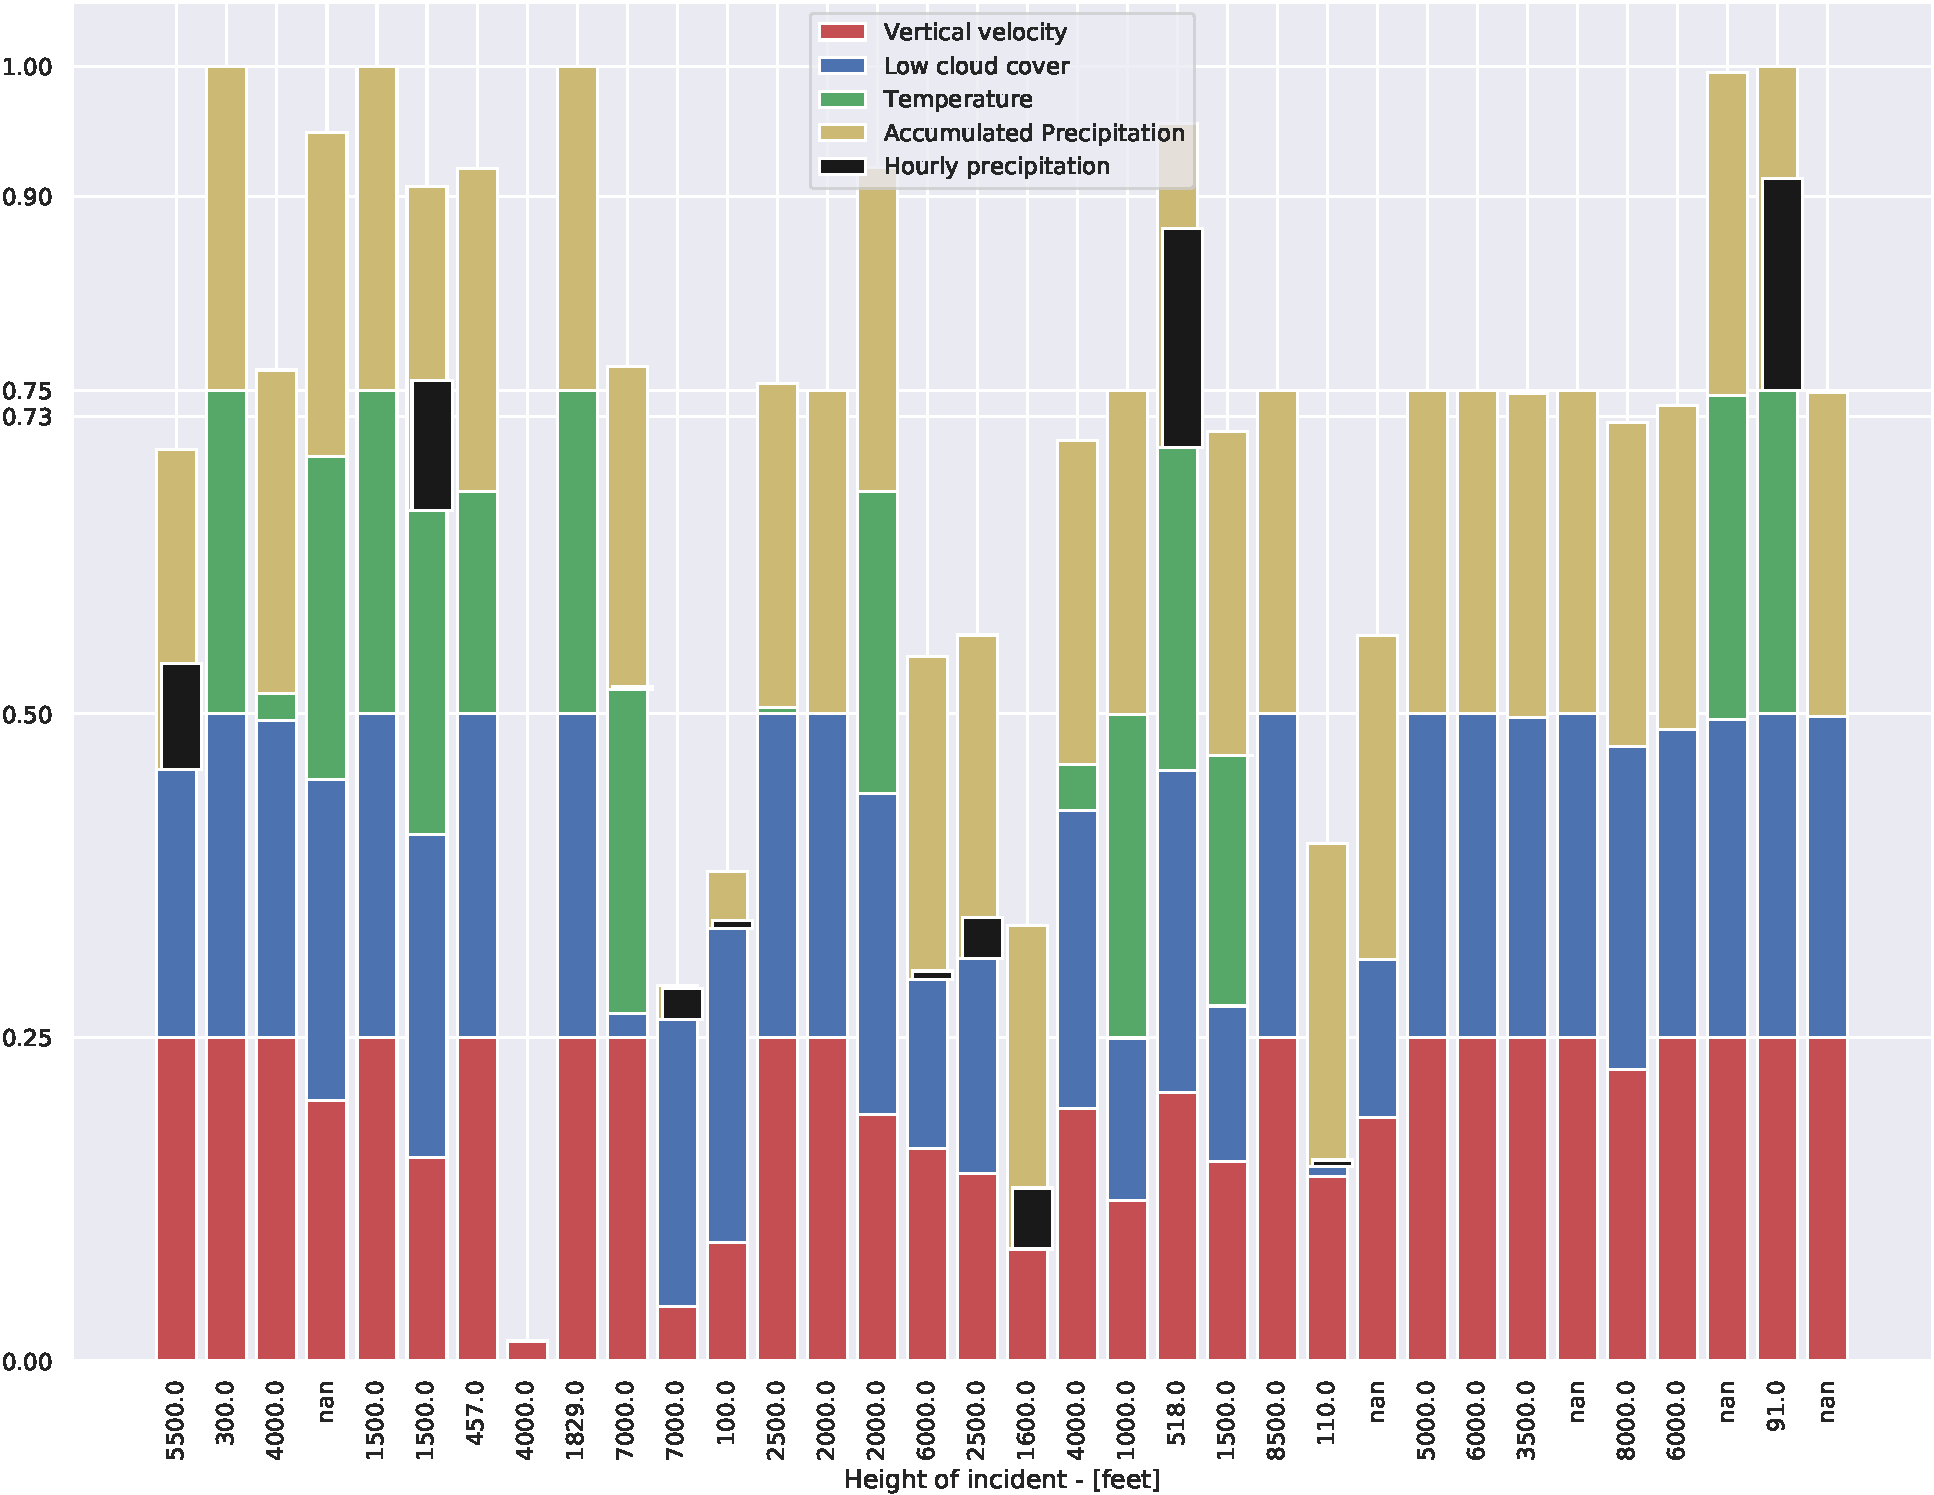
\includegraphics[width=\textwidth]{Figures/FWAccum.pdf}
    \caption{Contributions from the different sub-indices, for Fixed wing cases during the operational forecast. X-axis is height of incident in feet. Black on yellow is correction made by using the hourly precipitation instead of accumulated precipitation. Included are only cases from Avinor data set where position and height was available, for cases after November 2016.}
    \label{fig:FWAccum}
\end{figure}

\begin{table}[H]
    \centering
    \begin{tabular}{c|c|c|c}
        Forecast & With Accumulated & Without Accumulated & Missed \\ \hline
        >Yellow (0.73) & 22 & 21 & 14 (41.2\%)\\
        >Orange (0.90) & 10& 8& 25 (73.5\%)\\ 
        >Red (0.99) & 4& 3& 30 (88.2\%)\\
    \end{tabular}
    \caption{Amount of cases forecast in each risk category based on the $34$ Fixed wing cases in Figure \ref{fig:FWAccum}. A Red risk is counted in Orange, and Yellow.}    \label{tab:FWCont}
\end{table}

\begin{figure}[H]
    \centering
    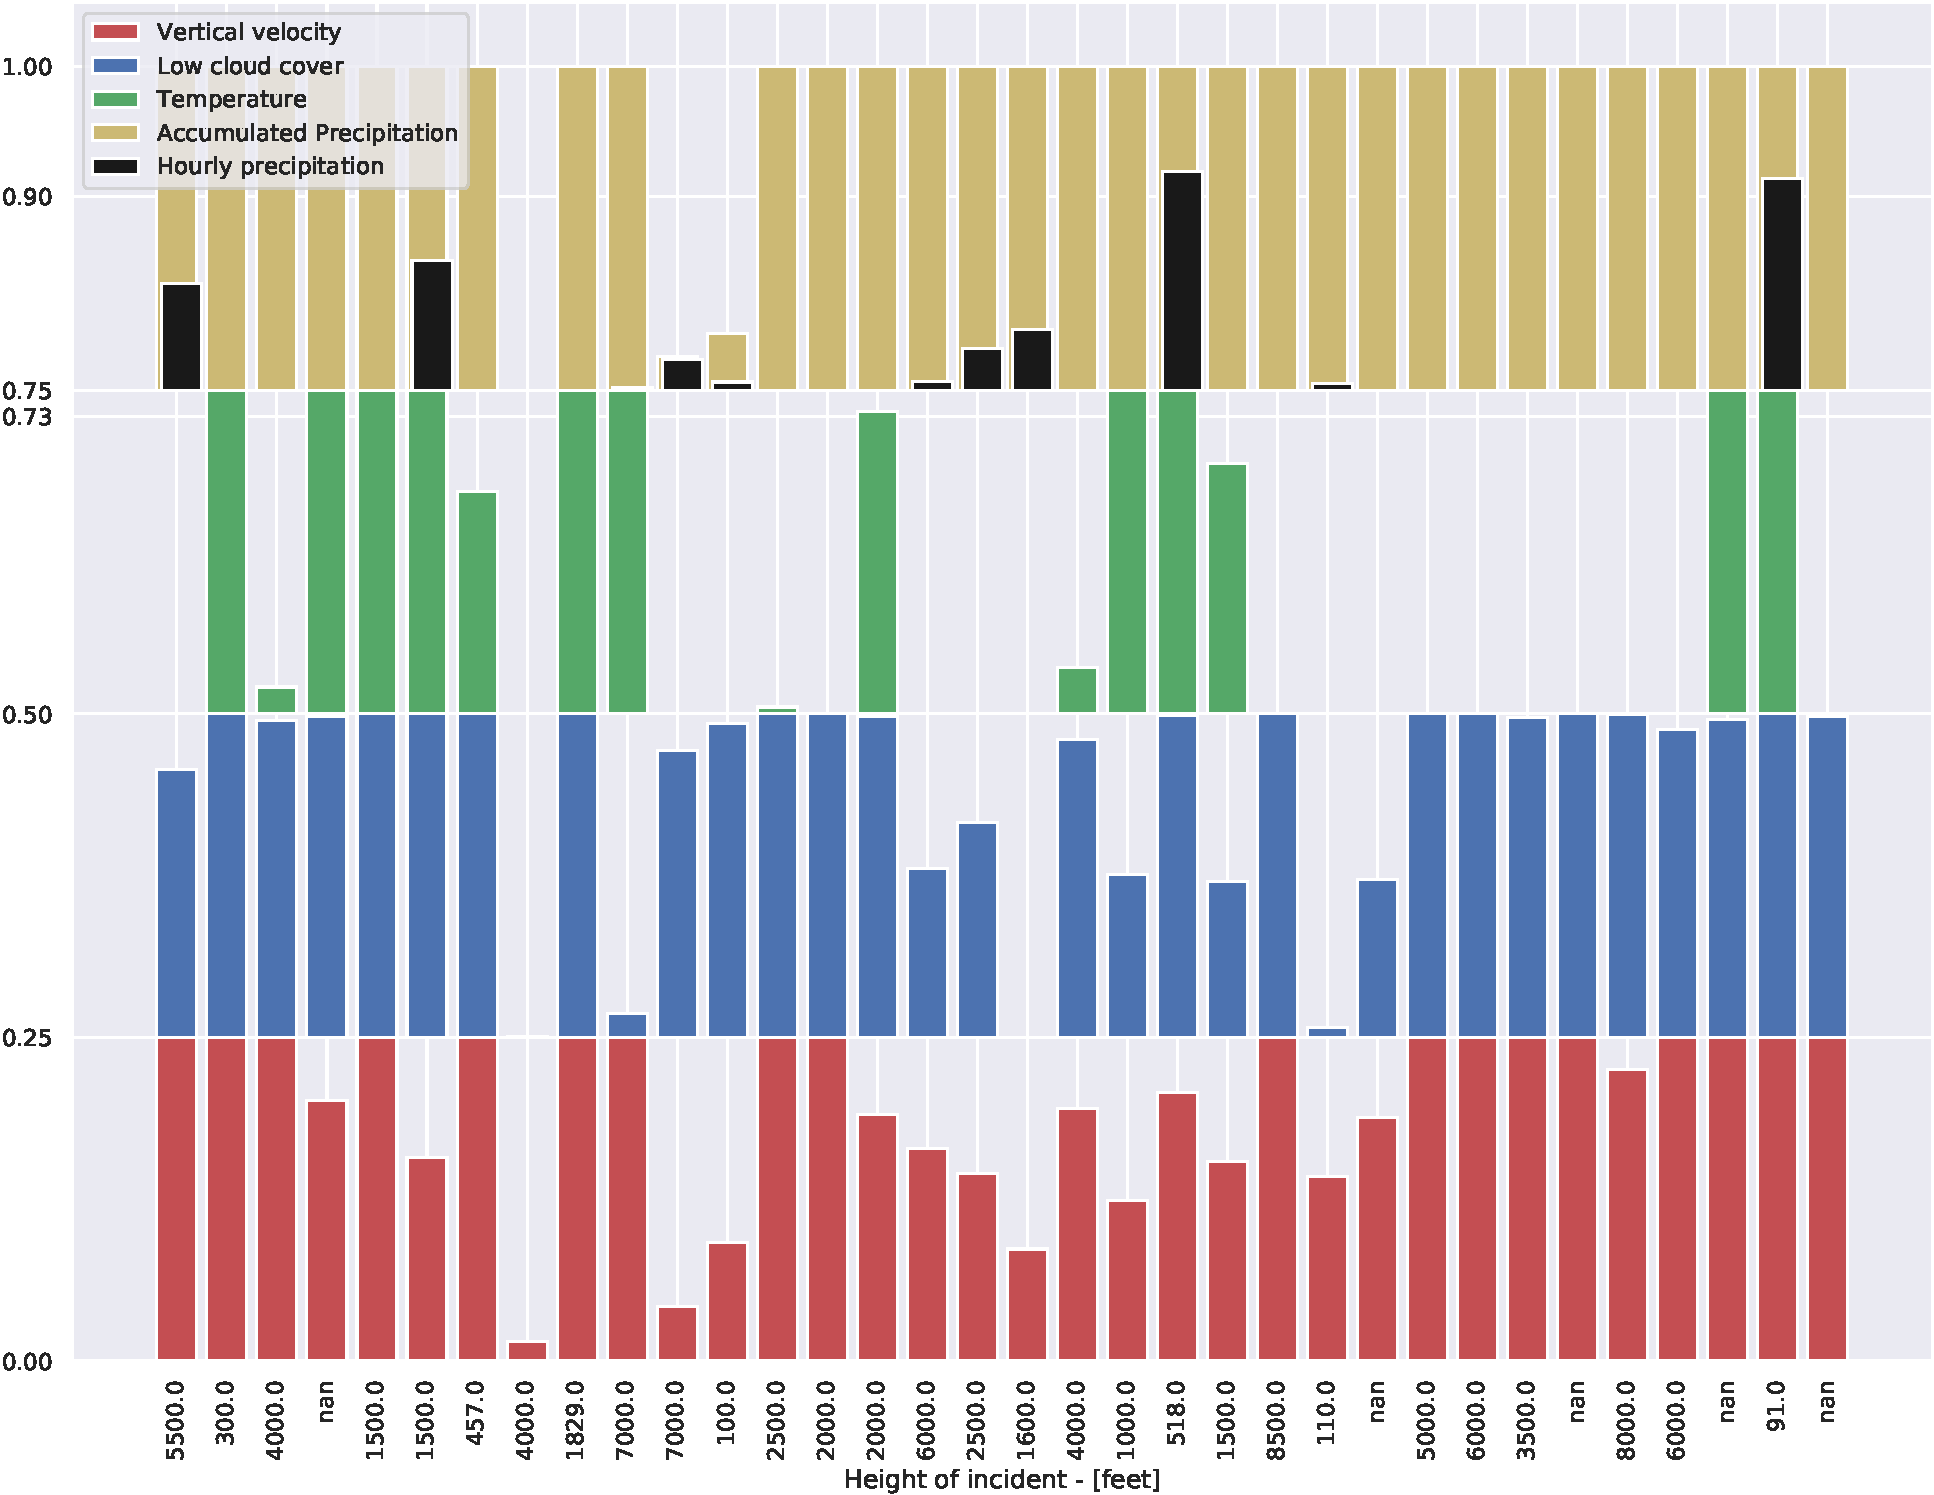
\includegraphics[width=\textwidth]{Figures/FWDecomp.pdf}
    \caption{Same as \ref{fig:FWAccum}, but clearly delineated between the sub-indices}
    \label{fig:FWDecomp}
\end{figure}

\cleardoublepage

\chapter{Conclusions}
\section{Are there still cases of Helicopter triggered lightning?}
\acrlong{htl} is still a recurring phenomenon, even after several years of forecasting the \acrlong{hti}. This is the reason why it is necessary to continue researching the phenomenon - the ideal scenario would be a forecast which prevented such cases altogether. 

This thesis found there to be an increase in cases in Norway after forecasting began in 2016. However, this may be seen as an artificial increase, as helicopter operators were in direct dialogue with the Meteorological Institute and more interested in reporting cases in order to improve the forecasting ability. It should also be noted that during the forecast period there have been no major incidents leading to major incidents. The cases happening were also found to be happening at lower temperatures than the expected 0$^{\circ}C$ isotherm. This was discussed in Section \ref{sec:avinor}: It is probably the result of forecasting removing the theoretical peak at 0$^{\circ}C$, where more major incidents would have happened.

\section{What meteorological phenomena are observed during triggered lightning incidents?}
To identify atmospheric conditions leading to a \acrshort{htl}, both METAR and composite plots were studied. This thesis found from both METAR and composite plots that convective precipitation and non-stratiform cloud types to be related to triggered lightning incidents. This thesis also reaffirms that the temperature during triggered lightning events were situated around -3 to 0$^{\circ}C$ for the altitude of the aircraft, both for the fixed wing and for the helicopter situation. It also found typical pressure patterns leading to geostrophic winds incident on coastal areas, suggesting convection due to convergence being important.

\section{How does the Helicopter Trigger Index perform when cases are happening?}

\section{In what ways can the HTL-forecast be improved?}

\section{Future research}
\cleardoublepage

\chapter{Discussion}
\cleardoublepage

\addcontentsline{toc}{chapter}{Bibliography}

\appendix
\chapter{Pressure versus model-level interpolation}
% remove comment if you wish to add Appendix to contentsline.
%\addcontentsline{toc}{chapter}{Appendix A: How to download ERA5 data}
\section{Temperature}
\begin{figure}
    \centering
    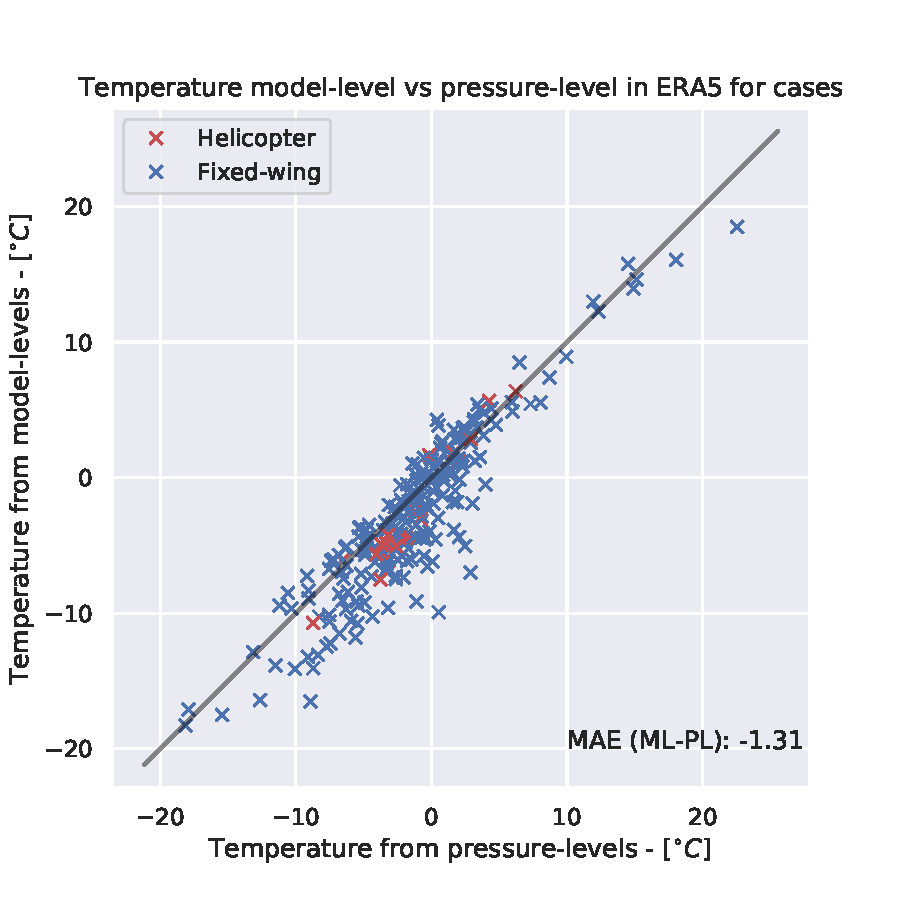
\includegraphics[width=0.8\textwidth]{Figures/mlvspl.pdf}
    \caption{Correlation between model-level and pressure-level interpolation of temperature from ERA5}
    \label{fig:mlvspl}
\end{figure}

\begin{figure}
    \centering
    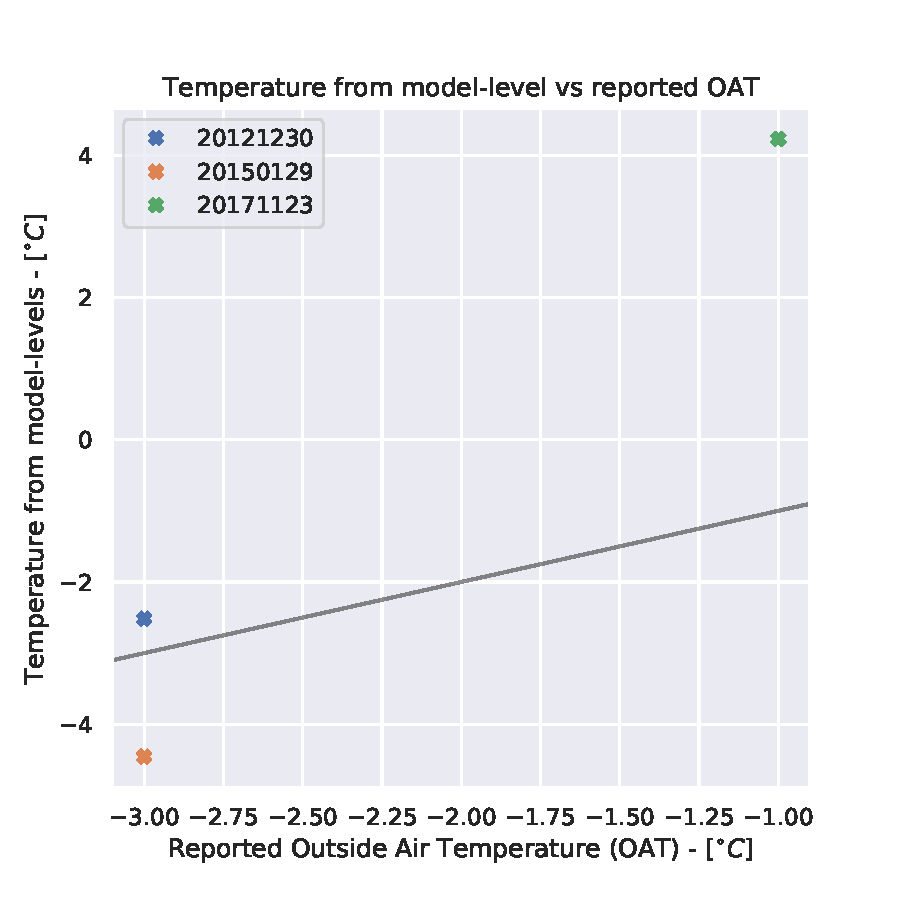
\includegraphics[width=0.5\textwidth]{Figures/mlvsoat.pdf}
    \caption{Correlation between model-level interpolation of temperature from ERA5 and observed Outside Air Temperature}
    \label{fig:mlvsoat}
\end{figure}

\begin{figure}
    \centering
    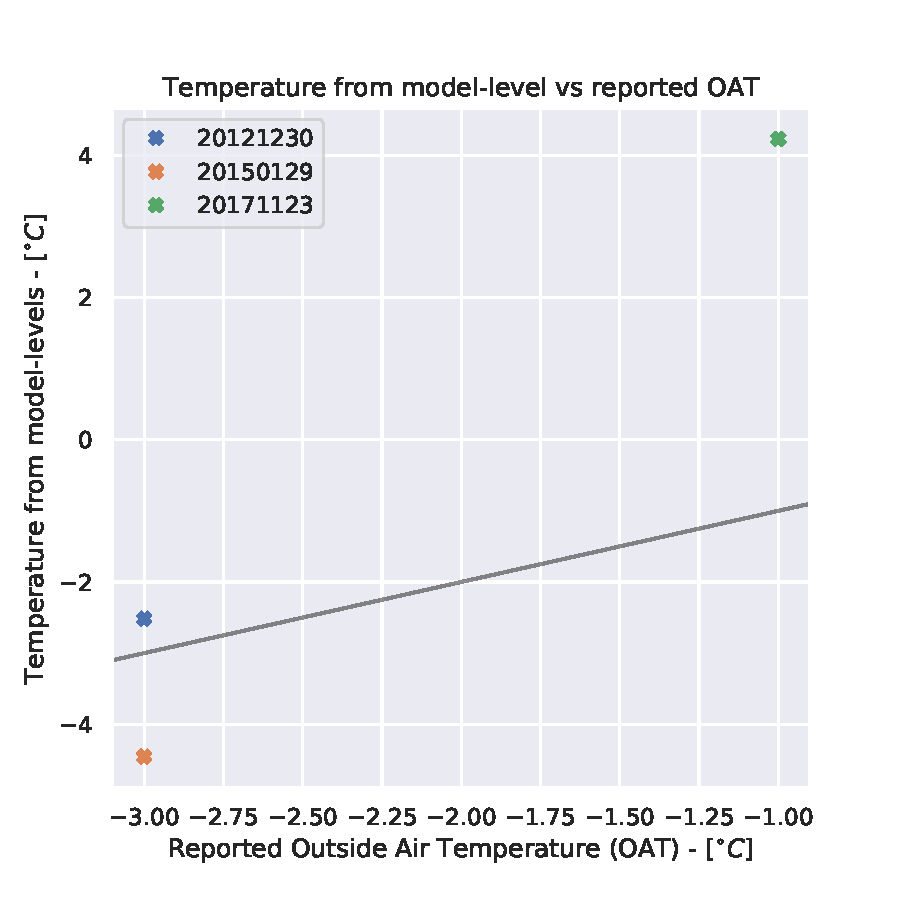
\includegraphics[width=0.5\textwidth]{Figures/mlvsoat.pdf}
    \caption{Correlation between pressure-level interpolation of temperature from ERA5 and observed Outside Air Temperature}
    \label{fig:plvsoat}
\end{figure}


\chapter{Operational categories of HTL-severity}
%\addcontentsline{toc}{chapter}{Appendix B: Additional figures}


\cleardoublepage

\printbibliography
\cleardoublepage

\end{document}
